\documentclass[11pt, a4paper]{article}

\usepackage{amsmath}
\usepackage{commath}
\usepackage{url}
\usepackage{cite}
\usepackage{color}
\usepackage{multirow}
\usepackage[margin=1.25in]{geometry}
\usepackage{graphicx}
\usepackage[T1]{fontenc}
\usepackage[utf8]{inputenc}
\usepackage{authblk}
\graphicspath{{./graphics/}}

\usepackage{subfiles}
\usepackage{blindtext}

\newcommand\T{\rule{0pt}{2.6ex}}       % Top strut
\newcommand\B{\rule[-1.2ex]{0pt}{0pt}} % Bottom strut

\newcommand{\gluex}{{\sc GlueX}\xspace}
\newcommand{\geant}{{\sc Geant}\xspace}
\newcommand{\babar}{BaBar\xspace}
\newcommand{\mydeg}{$^{\circ}$\xspace}
\newcommand{\myfar}{$^{\circ}$F\xspace}
\newcommand{\mycel}{$^{\circ}$C\xspace}
\newcommand{\eqdeg}{^{\circ}\xspace}
\newcommand{\deltall}{$\Delta$LL\xspace}
\newcommand{\bboson}{\emph{B} boson\xspace}
\newcommand{\bbosons}{\emph{B} bosons\xspace}
\newcommand{\gev}{~GeV\xspace}
\newcommand{\mev}{~MeV\xspace}

\title{GlueX DIRC Writeup}

\author[1]{M.~Patsyuk\thanks{mpatsyuk@mit.edu}}
\author[2]{R.~Dzhydaglo\thanks{r.dzhygadlo@gsi.de}}
\author[1]{J.~M.~Hardin\thanks{jmhardin@mit.edu}}
\author[1]{Y.~Yang\thanks{yunjiey@mit.edu}}
\affil[1]{\small{Massachusetts Institute of Technology, Cambridge, USA}}
\affil[2]{\small{GSI Helmholtzzentrum f{\"u}r Schwerionenforschung GmbH, Darmstadt, Germany}}

\date{\vspace{-5ex}}

\begin{document}

\maketitle

\section*{Abstract}

This note presents a description of the GlueX DIRC simulation and reconstruction software. The geometrical algorithm, based on the one developed for the BABAR DIRC, can be used as the baseline recontruction method for the start of the DIRC operation in 2018. The time imaging reconstruction has potential for better performance but requires additional development work. It performs better than the geometrical method for the existing timing resolution per photon of 1 ns. The KDE-based method is planned to be used for the tracks where the PID is not clear after the baseline reconstruction is run (on average, the resolution for the KDE-based method is 30{\%} better than for the geometrical reconstruction).



\vspace{8cm}
\begin{center}
Version 3.0
\end{center}

\newpage

\tableofcontents

\newpage

\section{Detector design}

This chapter will describe the purpose and general design of the \gluex DIRC.
\vspace{0.5cm}

The \gluex DIRC detector~\cite{dirc} is designed to improve particle identification (PID) capabilities in the forward region of the \gluex~\cite{gluex1, gluex2} detector located in Hall D at Jefferson Lab. The baseline PID in the forward region of the \gluex detector is done by a Time-Of-Flight (TOF) wall, which separates kaons from pions up to momentum around 2 \gev/c. The \gluex DIRC is designed to provide clean separation between kaons and pions with at least three standard deviations for momenta up to 4 \gev/c.

\begin{figure}[!htb]
\centering
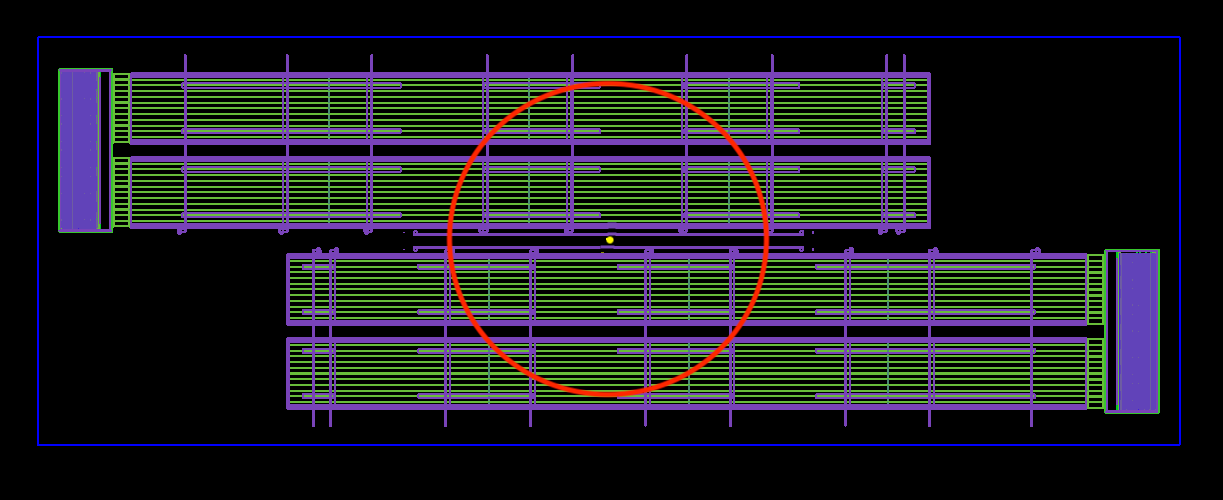
\includegraphics[width=0.9\textwidth]{pics/sim1.png}
\caption{\label{pic:sim}
The view (downstream the beam) of the \gluex DIRC optical system (from the simulation). The beam going into the page is shown in yellow. The red circle shows the polar angle acceptance ($11^{\circ}$ degrees).
The blue box around the detector is the auxiliary volume \texttt{DIRC} containing all the DIRC components, which can be activated/deactivated in the Hall D geometry to insert/remove the \gluex DIRC to/from the \gluex DIRC detector simulation.}
\end{figure}

The \gluex DIRC forms a wall about 5 m away from the target directly upstream of the TOF detector. The DIRC consists of four \babar DIRC~\cite{bdirc1} bar boxes and covers the polar angle range from 2\mydeg to 11\mydeg (see Fig.~\ref{pic:sim}). Two bar boxes located above the beam line are attached to a photon camera located to the left of the beam. Another pair of the bar boxes covering the acceptance below the beam line is attached to the second photon camera located to the right of the beam. The support structure of the DIRC (shown in Fig.~\ref{pic:support}) allows the pairs of bar boxes to swap out of the active area of the detector (see Fig.~\ref{pic:retracted}) for experiments requiring minimal material budget in front of the forward calorimeter.

The \babar DIRC bar boxes number 0, 1, 10, 11 (out of twelve) were designated for the \gluex DIRC. They were brought to Hall D by a truck from SLAC, where all the bar boxes had been stored after the \babar experiment was disassembled. The structure of a bar box is shown in Fig.~\ref{pic:bbox}. It is an isolated unit with $12$ long radiator bars ($35 \times 17.25 \times 4900 $ mm$^3$) inside. A small wedge is attached to the readout end of each radiator. Bar boxes are to be used without modifications, which means that the small wedges have to stay in the optical system of the \gluex DIRC.

\begin{figure}[h]
\centering
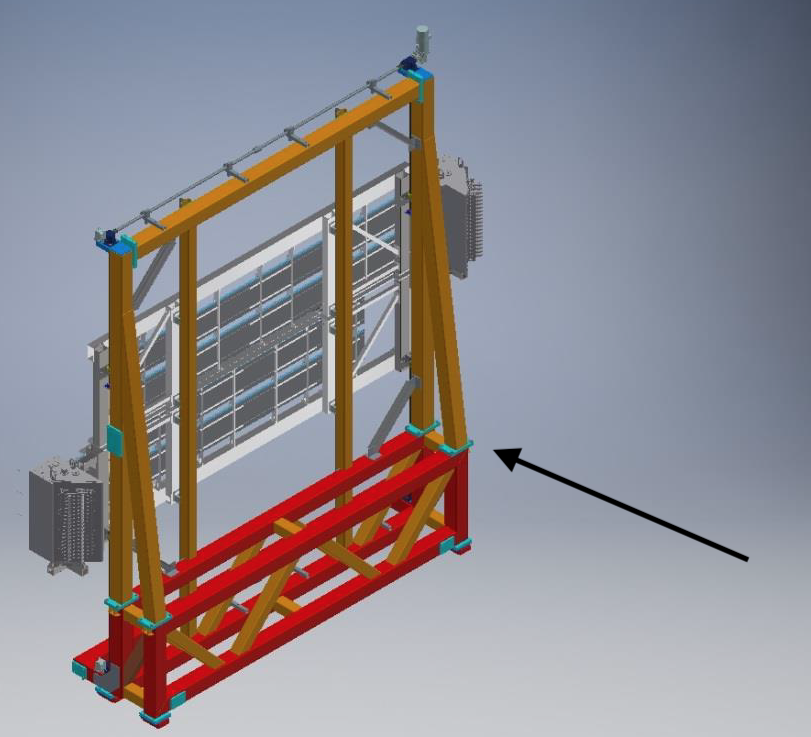
\includegraphics[width=0.6\textwidth]{pics/support.png} 
\caption{\label{pic:support}} A technical drawing of the support structure with the DIRC optical system installed. The bar boxes slide up and down within the orange frame. The beam is coming from the right.
\end{figure}

\begin{figure}[!h]
\centering
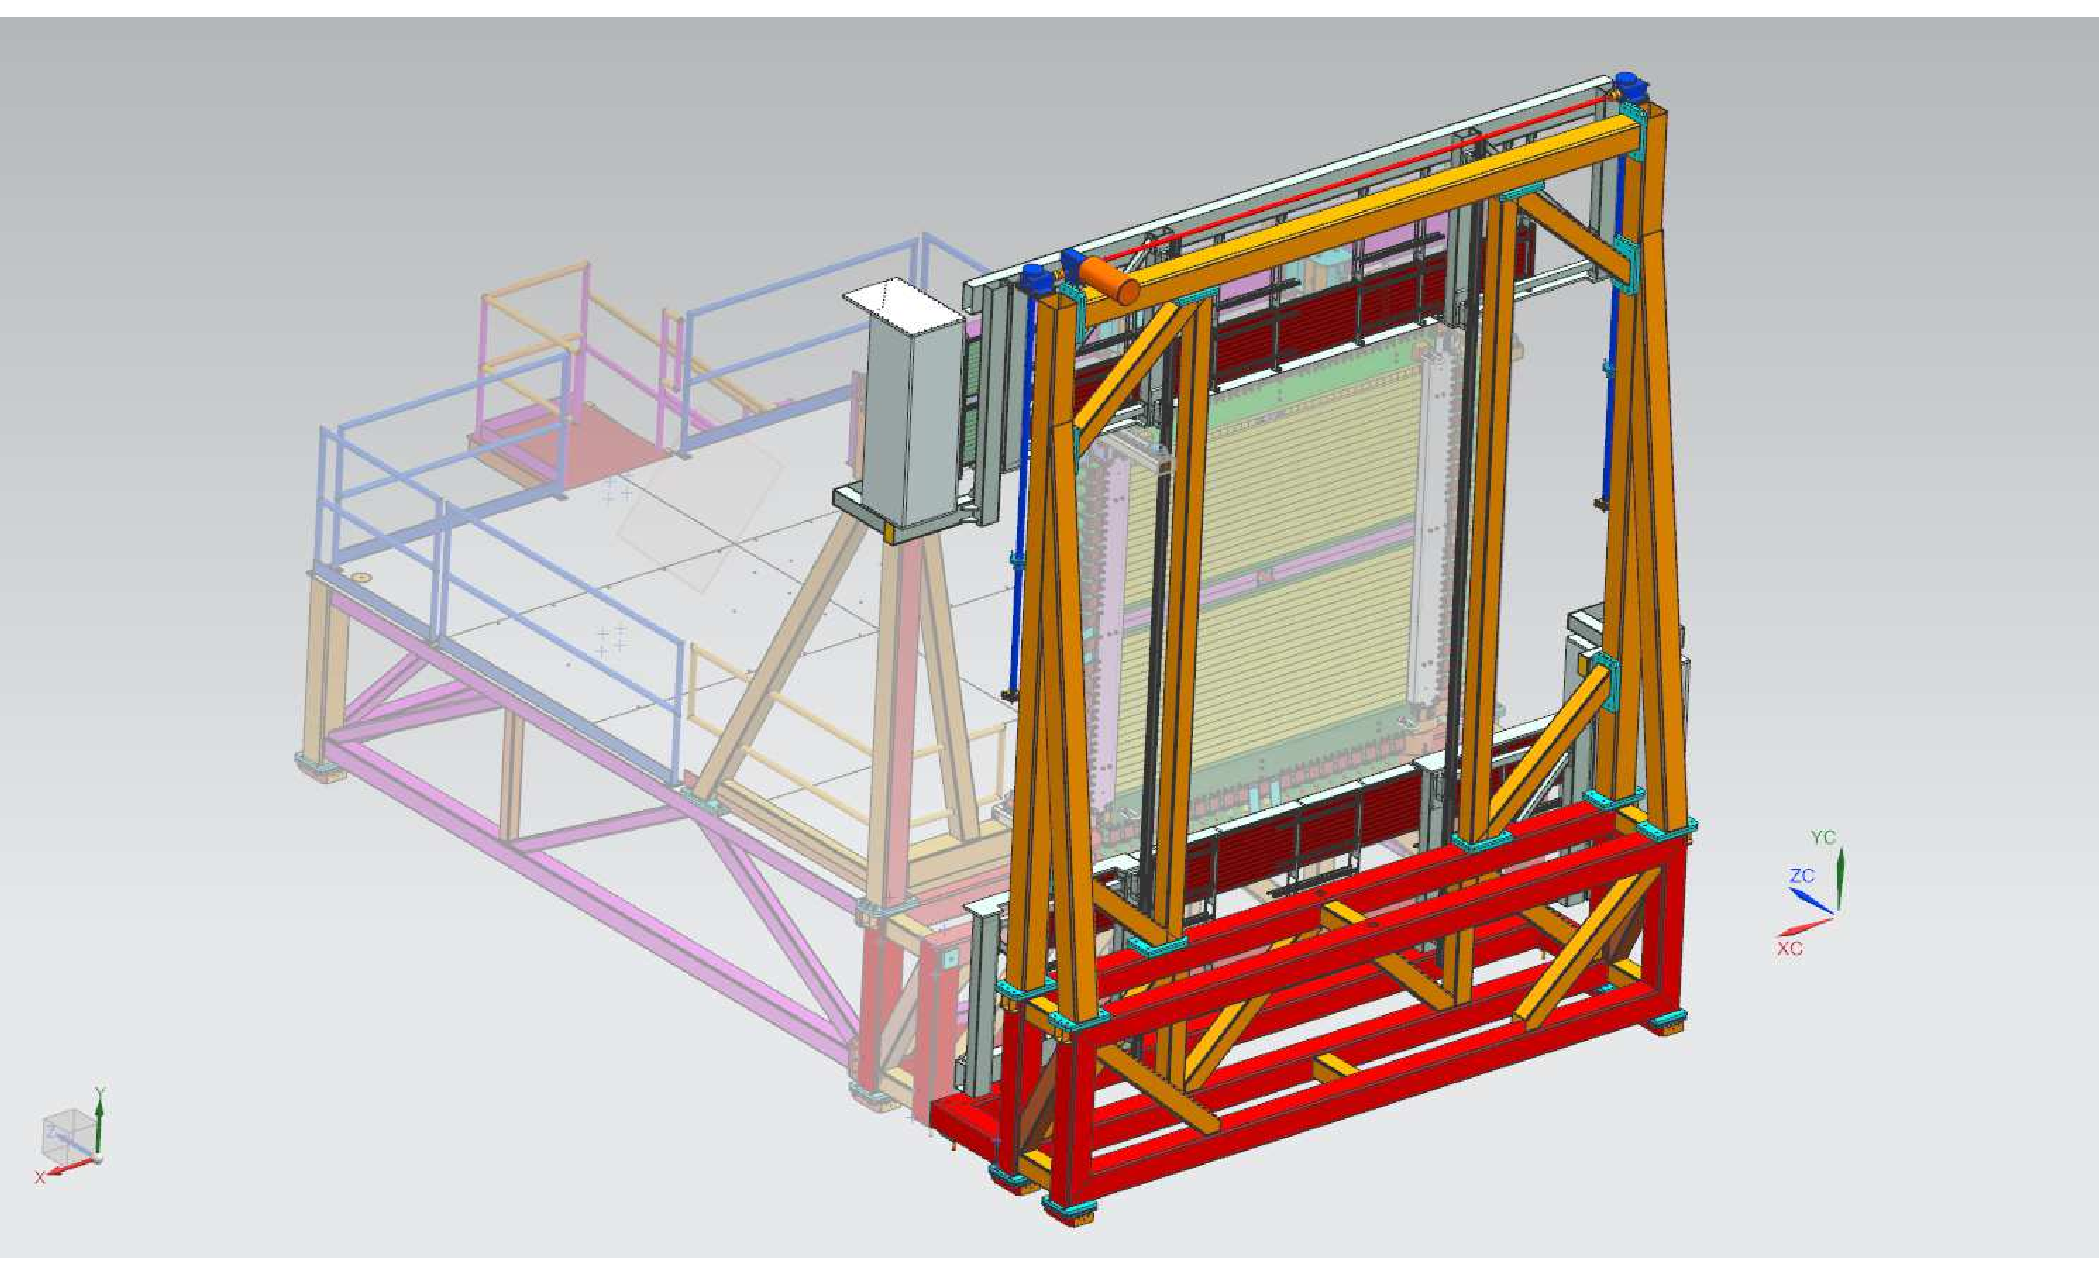
\includegraphics[width=0.9\textwidth]{pics/Full_Assy_Iso-retracted.pdf}
\caption{\label{pic:retracted}} A technical drawing of the support structure with the DIRC retracted. The beam is coming from the right. The active area of the Forward Calorimeter is shown behind the DIRC. The platform is for the other forward \gluex detectors.
\end{figure}

\begin{figure}[!h]
\centering
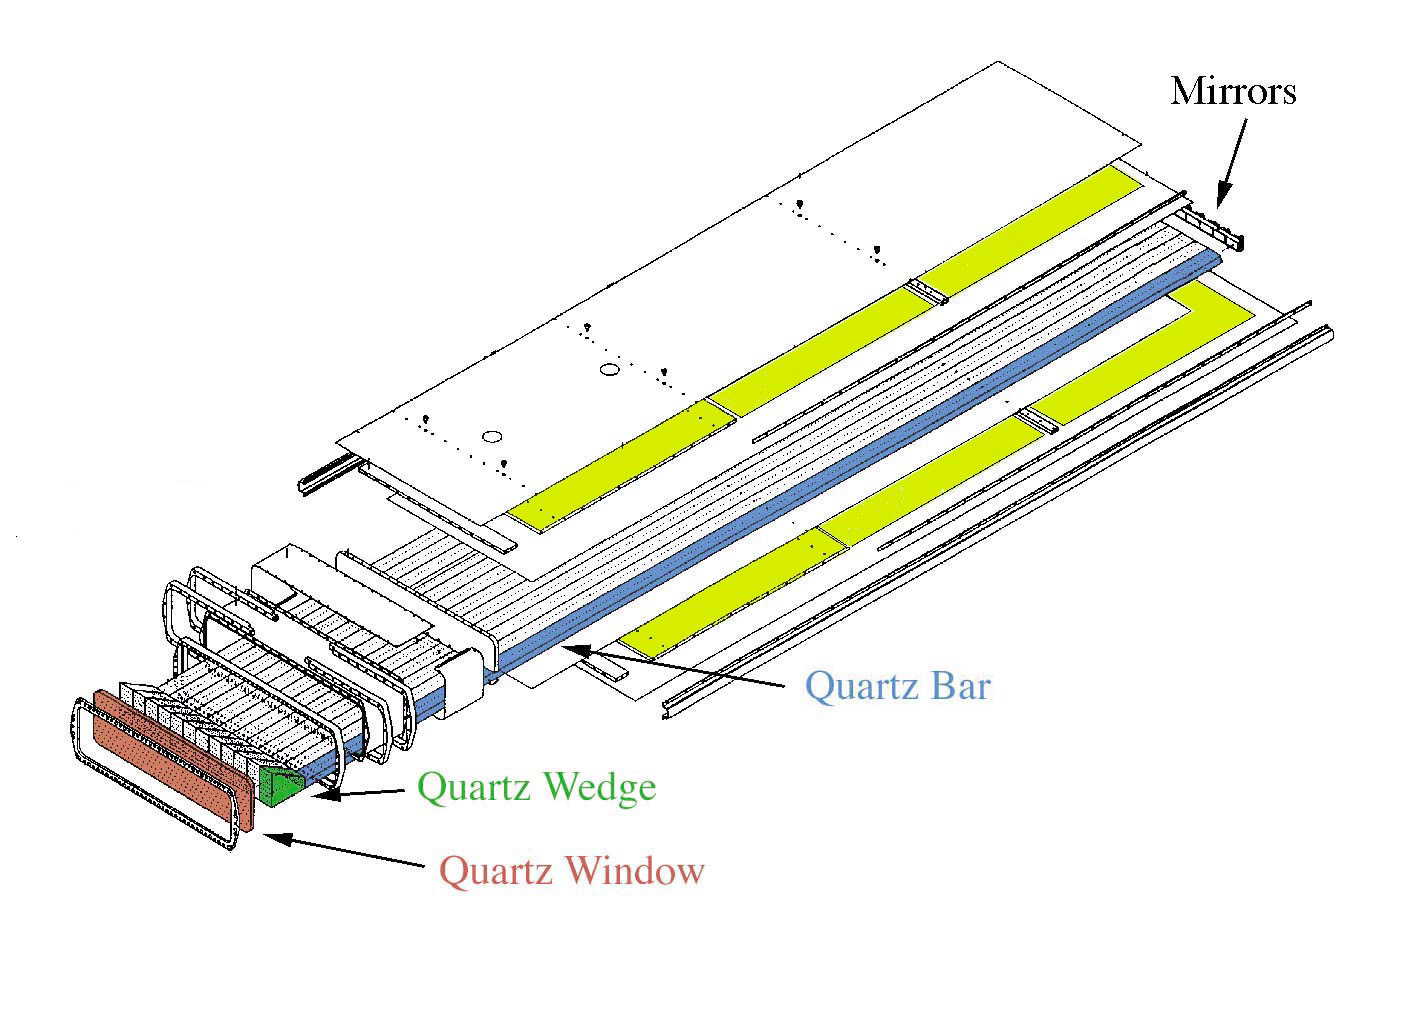
\includegraphics[width=0.8\textwidth]{pics/bab_col.jpg}
\caption{\label{pic:bbox} Schematic of the \babar DIRC bar box assembly. The single radiator bar is highlighted in blue, the small wedge -- in green.}
\end{figure}

\begin{figure}[!h]
\begin{center}
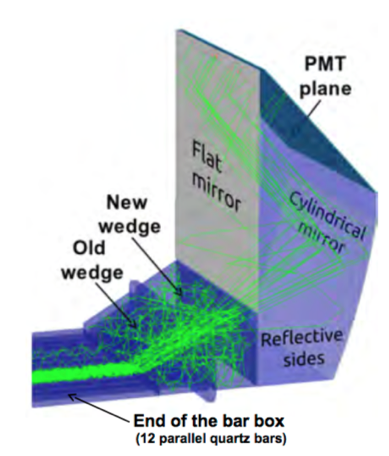
\includegraphics[width=0.3\textwidth]{pics/superB.png} \hspace{0.5cm} 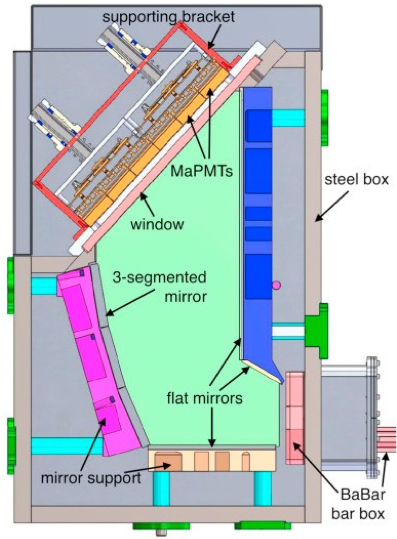
\includegraphics[width=0.4\textwidth]{pics/pc.png}
\end{center}
\caption{\label{pic:ob} Photon camera for the SuperB (left) and for the \gluex DIRC (right). The photon camera for the \gluex DIRC is a steel tank filled with distilled water with immersed mirrors to resemble the shape of the photon camera for the SuperB FDIRC.}
\end{figure}

The design of the photon camera is based on the SuperB FDIRC\footnote{FDIRC was designed to be the successor of the \babar DIRC, but the the SuperB project was cancelled in 2012.} prototype~\cite{fdirc} developed at SLAC. Figure~\ref{pic:ob} shows both cameras. The FDIRC photon camera design was based on compact focussing blocks made of fused silica, one for each bar box in a barrel. For the \gluex DIRC planar orientation one common camera, filled with distilled water, are used for two bar boxes together. This design with wider cameras (the width is $983$ mm) reduces the fraction of photons reflecting off the sides, simplifying the hit pattern and removing ambiguities in the reconstruction (reconstruction details see in Sec.~\ref{sec:gr} and Sec.~\ref{sec:ti}). Another important modification of the photon camera is the approximation of the cylindrical mirror by a set of three flat segments for simplicity in alignment and construction. 

The \gluex DIRC is read out by an array of Hamamatsu H12700 Multi-Anode PMTs (MaPMTs). Each photon camera is equipped with an array of $6 \times 18$ MaPMTs. One edge row of $18$ MaPMTs on each camera is substituted by dummies. This allows to use fewer PMTs. Simulation studies showed, that there is no performance loss due to removing one row of PMTs. The photosensors are coupled to the window of the optical box using custom-made silicone pads, which helps to minimise the photon loss between the window of the photon camera and MaPMTs. 

The electronics boards are the same as for the CLAS12 RICH in Hall B. They are compatible with the generic JLab DAQ systems.


\section{Simulation}
%\label{sec:sim}

A detailed physical simulation of the GlueX DIRC was developed using Geant4.
This chapter describes the details of the detector simulation, including the geometry, materials, and physical processes relevant for Cherenkov photon propagation. 

\subsection{Geometry}

The simulation of the \gluex DIRC detector within the \gluex software is based on {\geant}4 (\texttt{hdgeant4} package). The \gluex DIRC in simulation is defined by the geometry description (located in  \texttt{hdds/DIRC{\_}HDDS.xml}) and the functionality of the sensitive elements (described in \texttt{hdgeant4/src/GlueXSensitiveDetectorDIRC} class). 

The detector geometry is an important part of the detector simulation. It should represent all main features of the detector and contain all the elements responsible for the detector response. At the same time it should be simple and contain as few geometrical constituents as possible to keep the simulation fast. The \gluex DIRC geometry is shown in Fig.~\ref{pic:dirc}. Each volume is defined by its shape and material (the list of materials for the \gluex simulation is in \texttt{hdds/Material{\_}HDDS.xml}). 

\vspace{0.5cm}
Some basic rules for constructing a \geant geometry:
\begin{itemize}
\item \geant supports hierarchy, when daughter-volumes are located inside of a mother-volume.  Here one should make sure the daughter-volumes are completely within the mother volume. In case some part of a daughter-volume sticks out from the mother volume, a so-called ``overlap'' occurs. Such overlaps should be avoided. To check for overlaps, one has to uncomment the line \texttt{CHECK{\_}OVERLAPS{\_}MM} in the \texttt{GNUmakefile} in the top directory of the \texttt{hdgeant4} project and then recompile the \texttt{hdgeant4} project (for this do \texttt{touch src/HddsG4Builder.cc} and then \texttt{make} -- this only rebuilds classes that need to change)
\item The coordinates of the daughter-volume are set in the local coordinate system of the mother volume. The origin is at the center of the mother volume, if it is a box, and should be looked up in the {\geant}4 manuals otherwise
\item When creating a volume, e.g.
%\vspace{0.5cm}
\begin{center}
 \texttt{<box name="DCMV" X{\_}Y{\_}Z="560.0 250.0 150.0" material="OpticalAir" />} 
\end{center}
%\vspace{0.5cm}
\noindent its full (not half) dimenstions should be set. Here the box has dimensions of 560 cm x 250 cm x 150 cm.
\item Volumes can be grouped in assemblies called compositions. Inside a composition volumes are located with respect to the center of the composition. When the composition is placed inside the mother-volume, its center is placed with respect to the center of the mother-volume.
\end{itemize} 

\begin{figure}[!h]
\centering
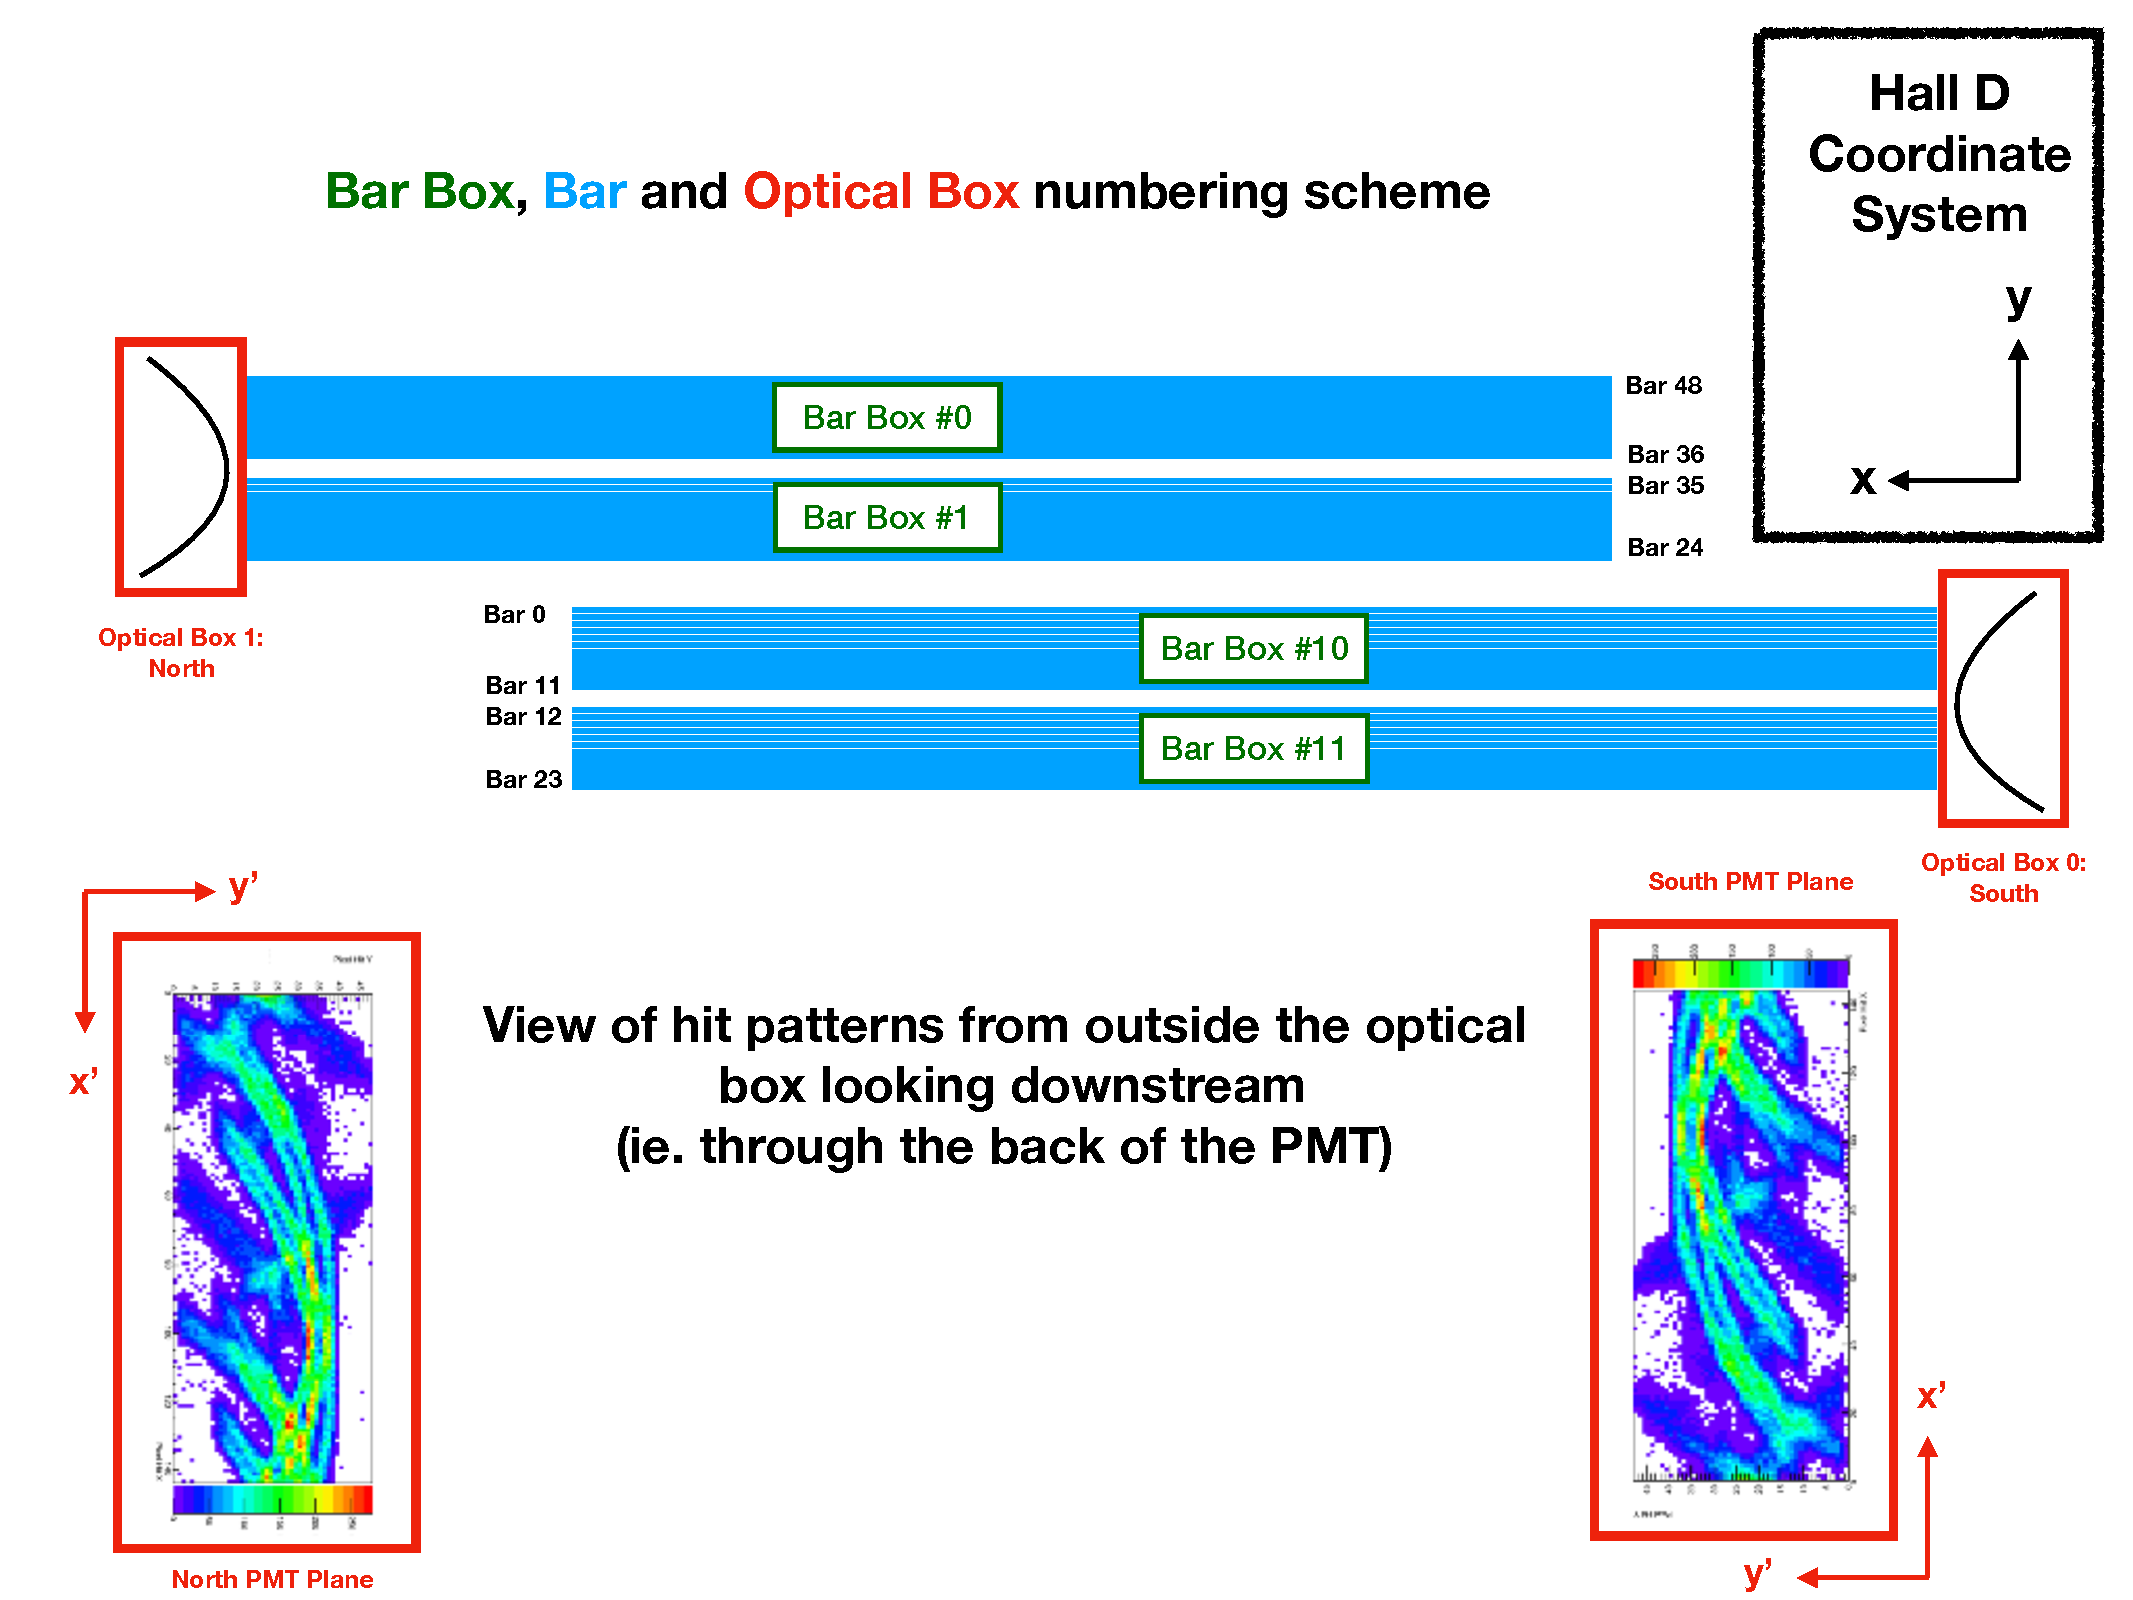
\includegraphics[width=0.98\textwidth]{pics/DIRC_Geometry11.pdf}\\
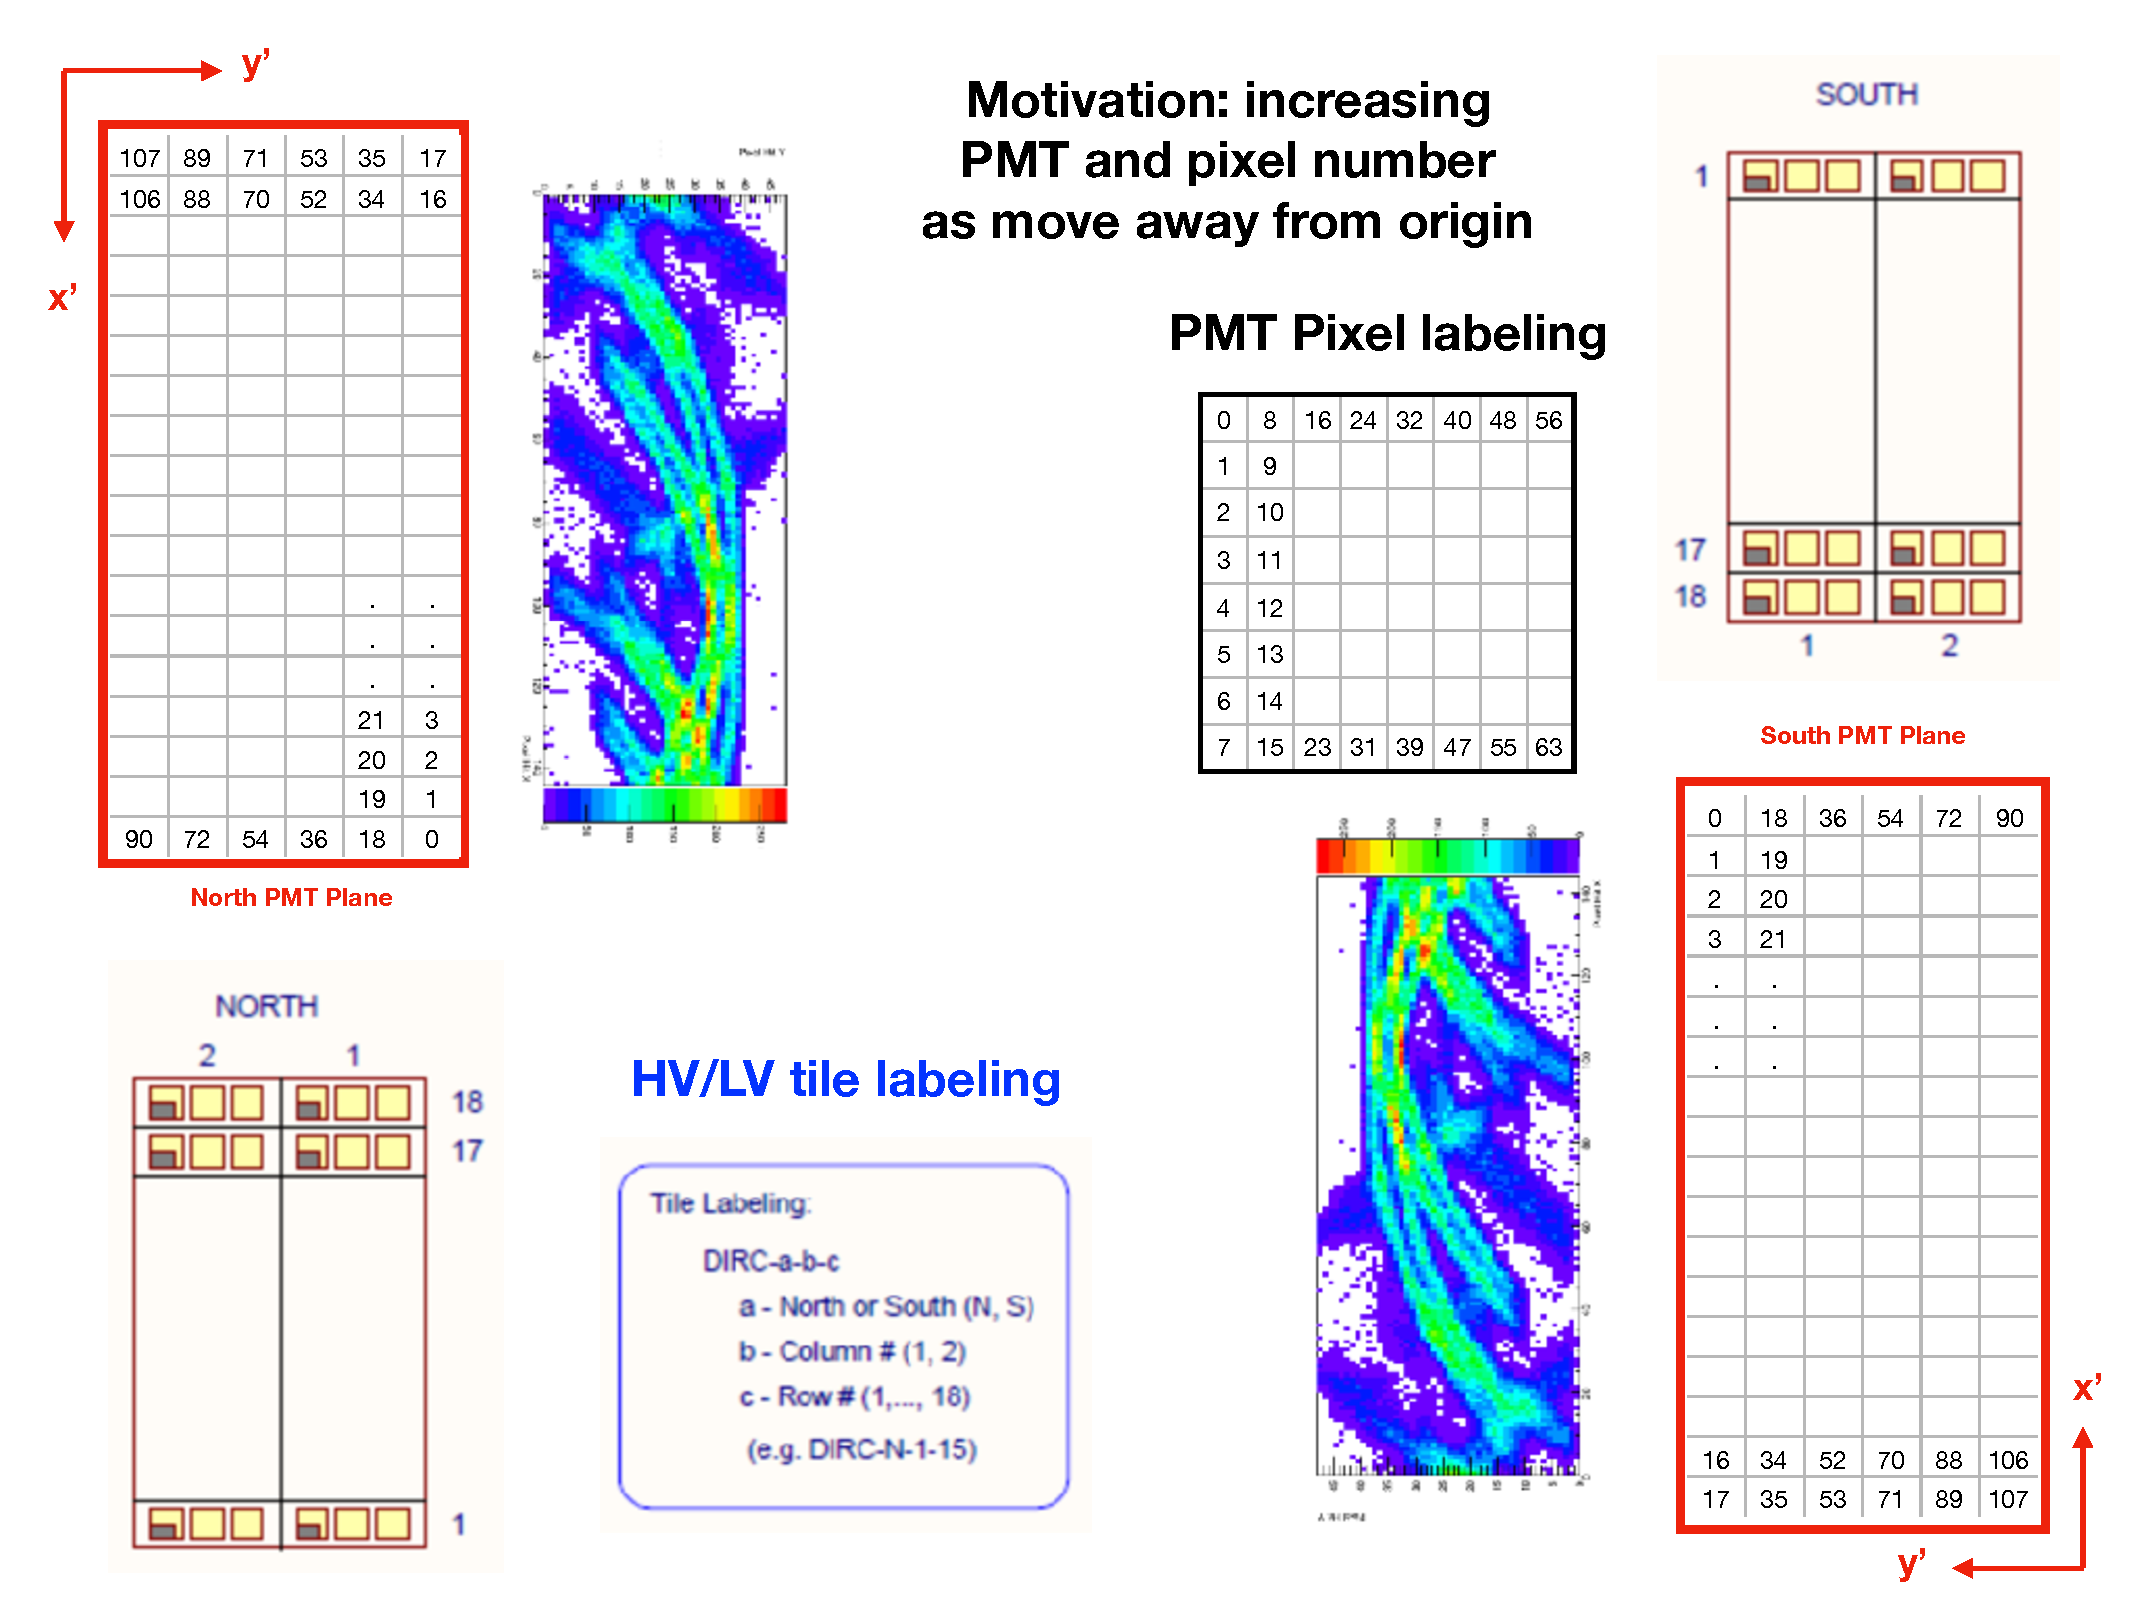
\includegraphics[width=0.98\textwidth]{pics/DIRC_Geometry22.pdf}
\caption{\label{pic:dircNumb}
Numbering schemes of the DIRC constituents.
}
\end{figure}

The DIRC can be activated or deactivated by commenting in/out the corresponding line in the \texttt{main{\_}HDDS.xml} file (lines 82-83): 

\vspace{0.5cm}
\begin{center}
 \texttt{<!- - To simulate DIRC hits uncomment the line below - -> \\
    <!- -posXYZ volume="DIRC" X{\_}Y{\_}Z="0.0 0.0 595.0" /- ->} 
\end{center}
\label{eq:line}
\vspace{0.5cm}

The \texttt{DIRC} object, which is placed inside the virtual Hall D when the line above is active, is an auxiliary volume in a shape of a rectangular block containing the DIRC detector (see Fig.~\ref{pic:sim}). Its coordinates are defined in the global coordinate system of the hall, in which the $z$ axis goes along the beam, $x$ axis is parallel to the floor (positive x is beam-left), and the $y$ axis is vertical (positive y is up). The target center is at $(0, 0, 65)$ cm. The center of the \texttt{DIRC} volume is at $z = 595$ cm.
Taking into account the z locations of the daughter volumes \texttt{DRCC} (composition holding the DIRC constituents), \texttt{DCML} (bar box), and \texttt{DCBR} (the radiator bar), the center of the radiator bar is currently at $z = 595 - 40 + 30 =585$ cm downstream the global 0. The distance from the center of the target ($(0, 0, 65)$ cm) is $585 - 65 = 520$ cm. The numbering schemes of individual volumes are represented in Fig.~\ref{pic:dircNumb}.

\begin{figure}[!htb]
\centering
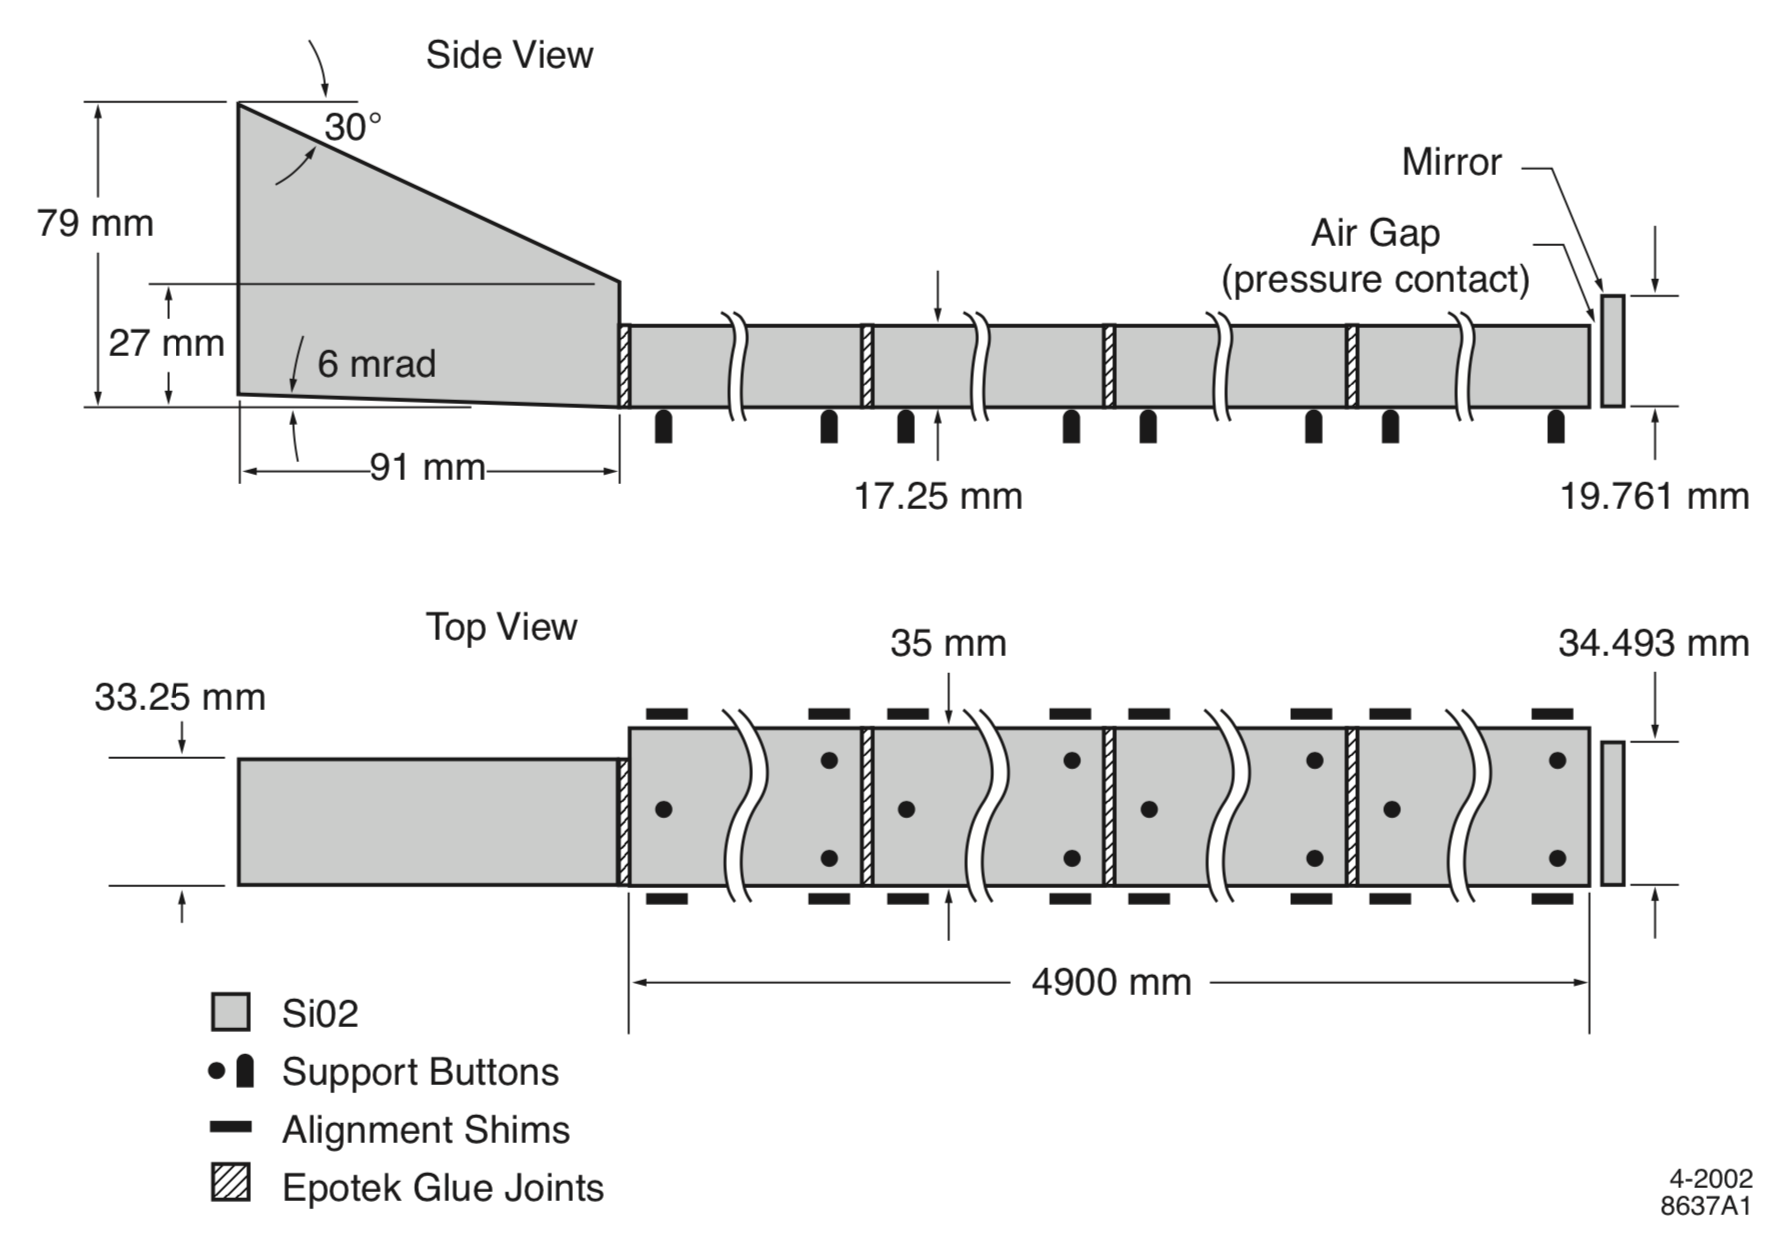
\includegraphics[width=0.9\textwidth]{pics/bars.png}
\caption{\label{pic:bar}
Schematic of the DIRC radiator bar in side and top view.
}
\end{figure} 

\begin{figure}[!h]
\centering
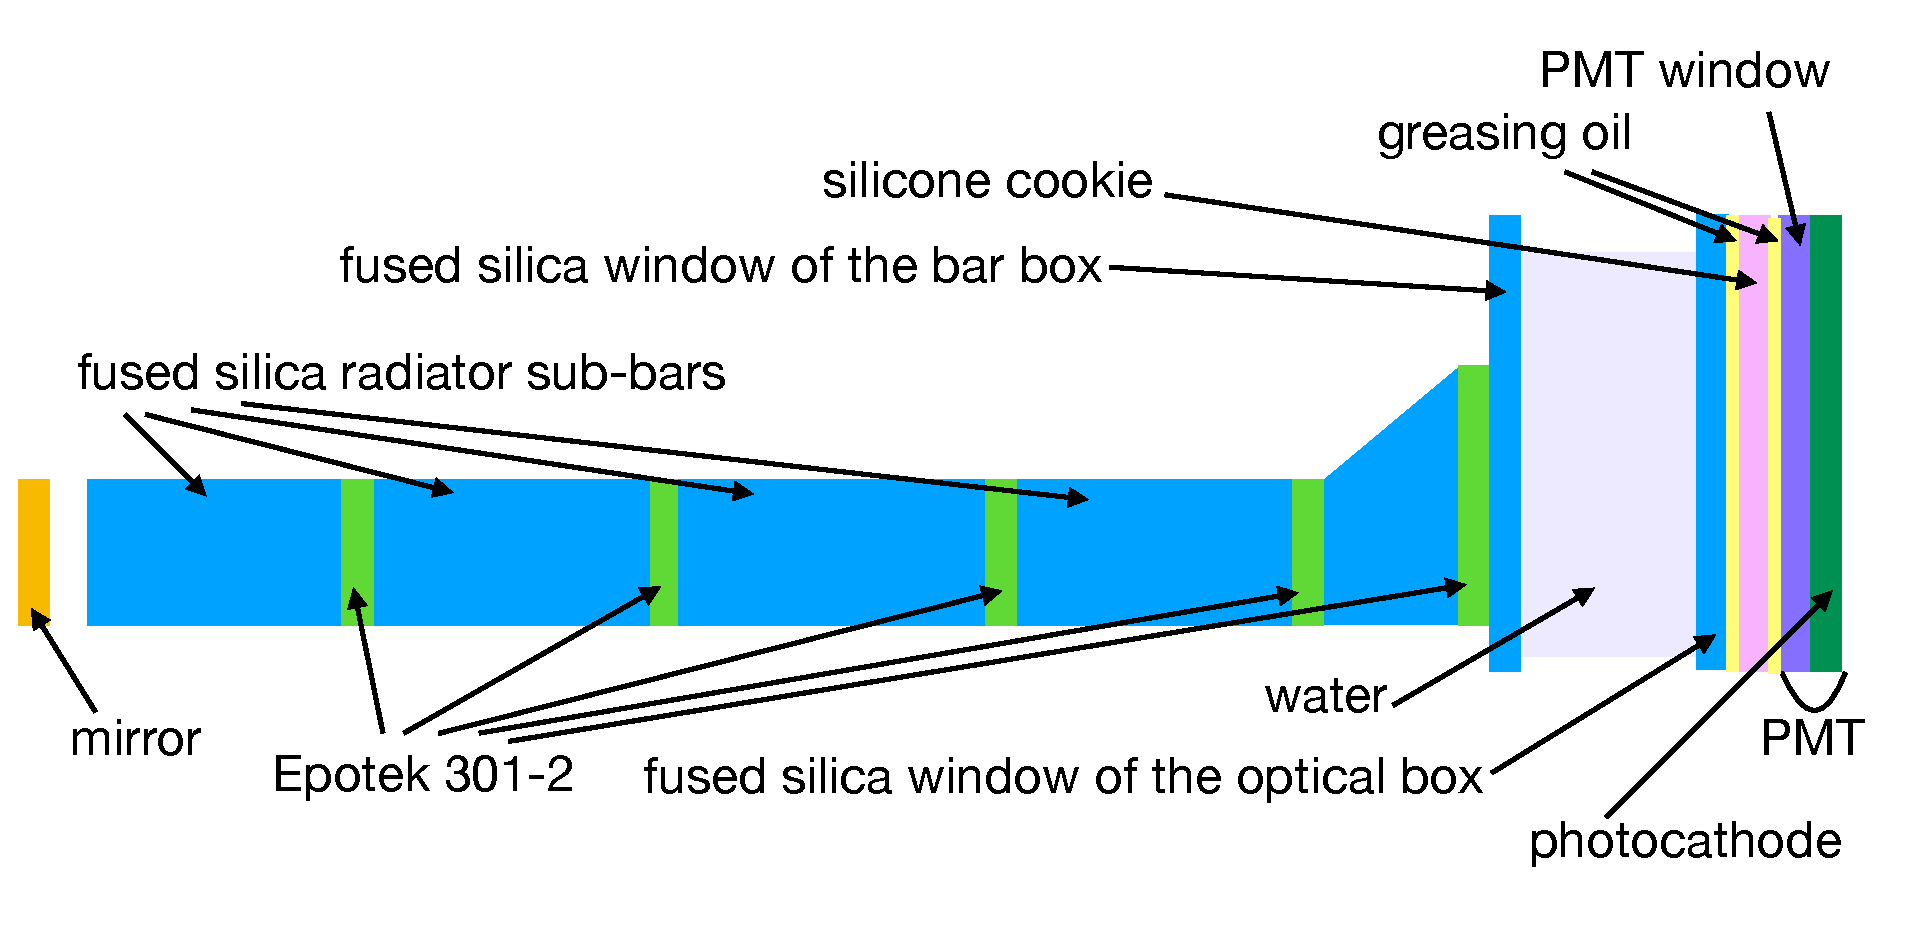
\includegraphics[angle=0,width=0.95\textwidth]{pics/struct3.pdf}
\caption{\label{pic:struct}
Schematic of one bar box in projection along the radiator length showing all the materials used for the optical system. Mirrors inside the optical box are omitted. The components are shown not to scale.
}
\end{figure}

The structure of the radiator bar is shown in Fig.~\ref{pic:bar}. The mirror at the end of the bar has pressure contact with the fused silica bar, which implies an air gap. In simulation there is an air gap of $0.1$ mm between the mirror and the radiator bar. The schematic of the \gluex DIRC functional optical elements, illustrating different materials used in the simulation, is shown in Fig.~\ref{pic:struct}. 
The average bar dimensions are $35 \times 17.25 \times 4900 $ mm$^3$. The \babar group shared a spreadsheet containing the actual dimensions of the radiators (and sub-radiators) inside every bar box. So that we implemented the real radiator dimensions in the simulation geometry. The spread within each dimension in cm (global c.s.):

\begin{align}
X &:  [122.41022, 122.4788] \\
Y &:  [3.31724, 3.49593] \\
Z &:  [1.57734, 1.71729]
\end{align}

The real radiators have not only slightly different dimensions, but also small variations on the angle between the adjacent faces. Those variations were not taken into account for the simulation, so that the radiations are perfect parallelepipeds.
The real radiators are not identical, and therefore should be aligned. The alignment convention in terms of the global c.s. is the following:

\begin{itemize}
\item X (along the radiator length): the radiators are aligned at the wedge exit. All the fused silica wedges are exactly the same and all the glue layers (for details see Fig.~\ref{pic:bar} or~\ref{pic:struct}) have the same thickness. As a result, the radiator end equipped with a flat mirror can have slightly different x coordinate.
\item Y (vertically): this dimension is the most critical due to the stress induced by the gravitational force. The radiators are aligned at the lower edge. The lowest bar in a bar box is supported by rubber buttons (see in black in Fig.~\ref{pic:bar}), the other eleven bars are resting on top of the first bar and separated from each other by special plastic spacers. The custom size of the spacers ensures the alignment of each bar in y at the lower edge. The position of the individual bar box within the \babar DIRC barrel defined which way the radiators inside the box are aligned in y. 
The \babar bar boxes number 00, 01, 10, 11 satisfied the alignment condition for the GlueX arrangement.
\item Z (along the beam): the radiators are aligned at the downstream side. This is the \babar legacy too: to make sure all the radiators in a barrel shape are at the same radius, they were aligned together with the wedges at the bottom side as shown in e.g. Fig.~\ref{pic:struct}.
\end{itemize}

The glue layers in (y,z) plane match the size of the larger bar/wedge. The size of the air gap in (y,z) between the radiator and the flat mirror matches the size of the radiator.

Realistic transport of Cherenkov photons through the optical elements of the detector from production to detection is essential for the DIRC simulation. Figures~\ref{pic:dirc} and~\ref{pic:obg} show that the current detector geometry matches the CAD technical drawings.

\begin{figure}[!h]
\centering
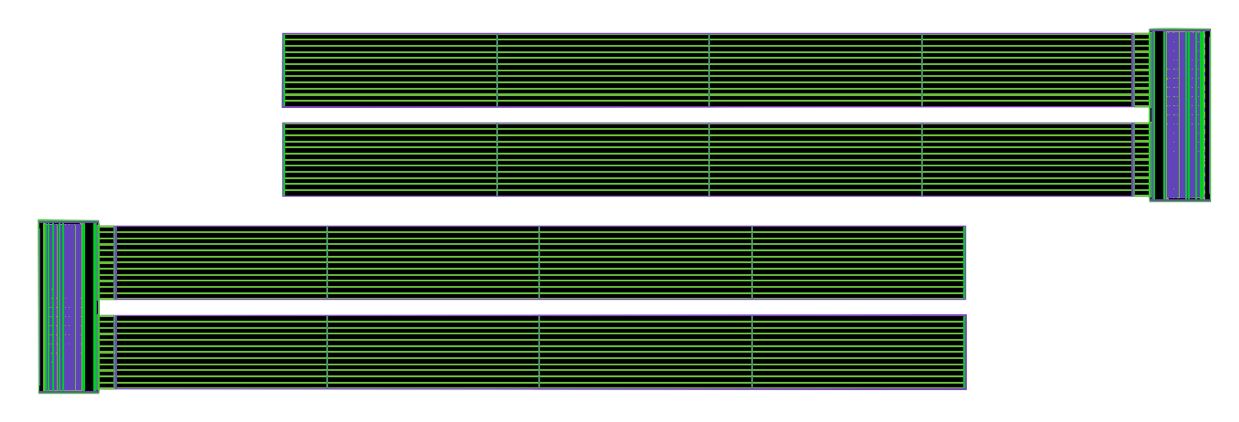
\includegraphics[width=0.8\textwidth]{pics/bars1.png}\\
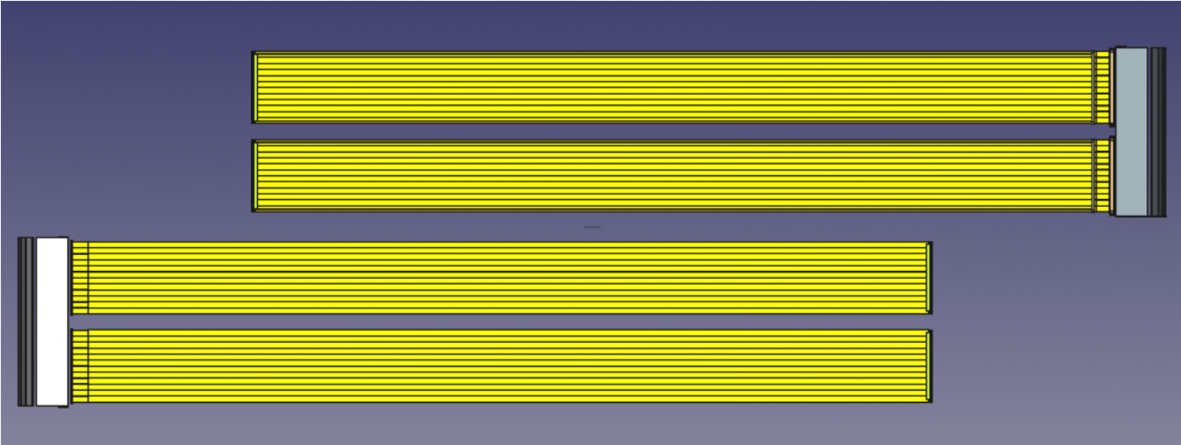
\includegraphics[width=0.8\textwidth]{pics/bars2.png}
\caption{\label{pic:dirc}
Simulation (top) and CAD drawings (bottom) of the \gluex DIRC. Upstream view.
}
\end{figure} 

\begin{figure}[!h]
\centering
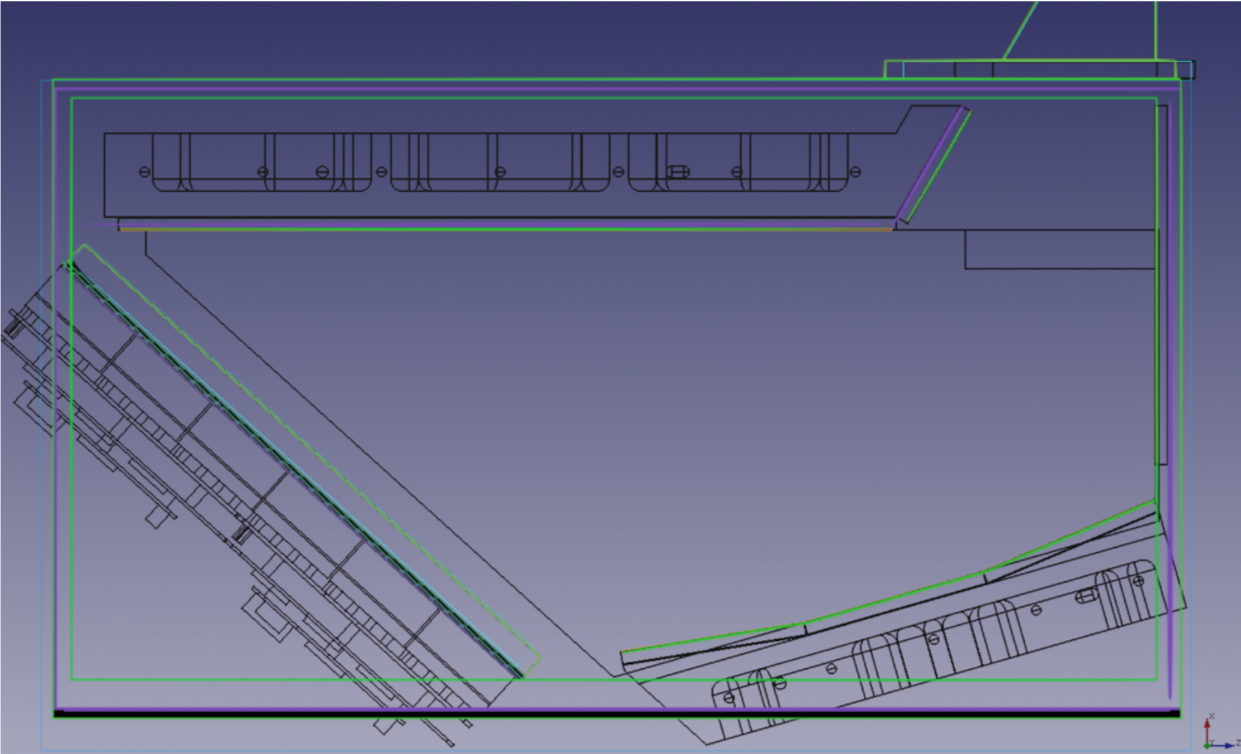
\includegraphics[width=0.8\textwidth]{pics/obgeom.png}
\caption{\label{pic:obg}
Geometry of the optical box overlayed with the CAD drawings illustrating the same locations of the mirrors. The optical elements are shown in green for the simulation and in black for the technical drawings.
}
\end{figure}

The photosensors are implemented in a simplified way. One MaPMT is basically a stack of two layers: a borosilicate window and a bialkali photocathode, so that photons sequentially propagate through them (see Fig.~\ref{pic:struct}). The bialkali photocathode is set as a sensitive material for \geant 4, which means, that when a photon enters this volume, a special function is called, which writes out the detector signal. The functionality of the sensitive elements of the \gluex DIRC is described in \texttt{GlueXSensitiveDetectorDIRC} class. All the 6 $\times$ 18 PMTs for each optical box are present in the simulation, which means that in order to account for dummies, one needs to manually mask those PMTs. The map of the dummies for the Spring 2019 run is shown in Fig.~\ref{pic:dummies}.

\begin{figure}[!h]
\centering
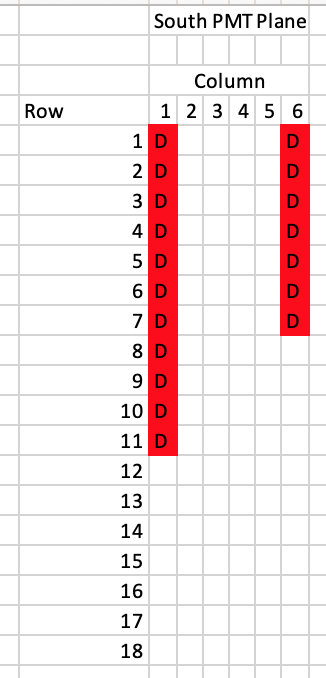
\includegraphics[width=0.3\textwidth]{pics/dummies.png}
\caption{\label{pic:dummies}
Locations of the dummy blocks (red) on the bottom (South) optical box for the 2019 Spring run, which is the technical run for the DIRC.
}
\end{figure}

The aluminum support structures located in the acceptance of the DIRC (shown in Fig.~\ref{pic:sim} as purple bars) and bar box internal aluminum supports including cross-beams, aluminum sheets and side edges are included in the simulation. They ensure proper material budget in front of the forward calorimeter.

%\input{pmt.tex}

\subsection{Physical processes}

The general physical properties of the media (such as density, atomic weights, atomic numbers etc.) are used by {\geant}4 to simulate interactions of the particles with detector materials (e.g. Bremsstrahlung, ionization, production of secondary particles). If a material has, in addition, Cherenkov properties, then a particle can emit Cherenkov photons inside this material. The expectation value of the number of Cherenkov photons emitted per unit of trajectory $dN/dx$ is calculated according to the Frank-Tamm equation. During the propagation process of a charged particle inside the material with Cherenkov properties the number of photons produced within each step is generated according to a Poisson distribution with the mean of $\langle n \rangle = L_{step} \cdot dN/dx$. After the photons are produced they are propagated individually through the detector materials. The particles are transported inside the detector volume in an iterative process to discrete positions with a certain step size. At each of these positions a detector-specific routine is called by the {\geant}4 in order to process the simulated information inside its sensitive volumes. There, the current particle state (e.g. momentum, type, and mother-daughter relation) and the relevant processes during the current step (e.g. reflection, refraction) are available.

A high momentum charged particle produces at the order of $1000$ photons per cm of fused silica in the wavelength range $(300-700)$ nm. Only $30-60$ of them are expected to be detected. Typical Cherenkov photon energies are in the range of few eV. For proper estimation of the detector performance it is very important to predict realistic photon yields. Common reasons why a Cherenkov photon is not detected are the following:

\begin{itemize}
\item The material, where the Cherenkov photons is produced or currently propagating, might be non-transparent for the given wavelength -- the photon stops (after some distance, depending on the defined absorption length as a function of wavelength for the given medium);
\item The photon does not satisfy the total internal reflection condition at the border between the radiator and the surrounding air or nitrogen (and other interfaces) -- the photon leaves the radiator (or, more generally, the optical system of the detector) and is lost;
\item Some photons are reflected back on an interface between media with different refraction indices -- the photon is trapped inside some volume (or group of volumes);
\item The photon is not detected because of the photon detection efficiency of the sensors (the quantum efficiency for H12700 MaPMTs is shown in Fig.~\ref{pic:qe}) or the transport efficiency in the radiator (described below)  -- the photon reaches the photosensor, but is not detected.
\end{itemize}

The physical processes in the materials are simulated by {\geant}4 based on the Cherenkov properties. The processes of total internal reflection, chromatic dispersion, transmission, and absorption of Cherenkov photons inside the optical elements of the \gluex DIRC are treated by {\geant}4, too.

A fraction of Cherenkov photons emitted by a charged particle, gets trapped inside the radiator due to the total internal reflection effect. They need to be transported from the origin to the readout end of the radiator bar. Cherenkov photons usually undergo about several hundreds internal reflections inside a long \babar DIRC bars on the way towards the readout end. The sides of the radiator in the reality are not perfect, and surface roughness causes a photon to get scattered in a random direction or escape from the radiator. In the simulation the radiator sides are perfectly polished leading to the fraction of transported photons to be $100\%$. In general, there are two ways to implement realistic transport efficiency into the simulation:

\begin{itemize}
\item The functionality of {\geant}4 (unlike {\geant}3) allows definition of an ``optical surface'' between two media with custom properties such as reflectivity and roughness. Then at each reflection off the radiator side, {\geant}4 decides according to the surface properties, to stop the photon or continue its transportation. It might be not straightforward to implement experimental results of the surface roughness measurements and make sure the simulation agrees with the measured data.
\item Transport efficiency can be calculated at the production stage for each photon based on the reflection probability and the total number of reflections off the sides. This speeds up the simulation. Also, the photon transport efficiency, which includes effects from the surface roughness and sub-surface damage, was experimentally measured for the \babar DIRC bard for several wavelength~\cite{roughness} and is, therefore, easy to implement.
\end{itemize}

We decided to follow the second method and apply the transport efficiency at the production stage as the following. The probability $P$ for a single reflection on the radiator side depends on the photon wavelength $\lambda$, incident angle of the photon $\alpha$, refraction index $n$, and the surface roughness $r$. According to scalar theory~\cite{scalar}:

\begin{equation}
P \approx  1 - \left( \frac{4\pi \cdot r \cdot \cos(\alpha) \cdot n(\lambda)}{\lambda} \right)^{2}, r \ll \lambda
\end{equation}

\begin{figure}[!h]
\centering
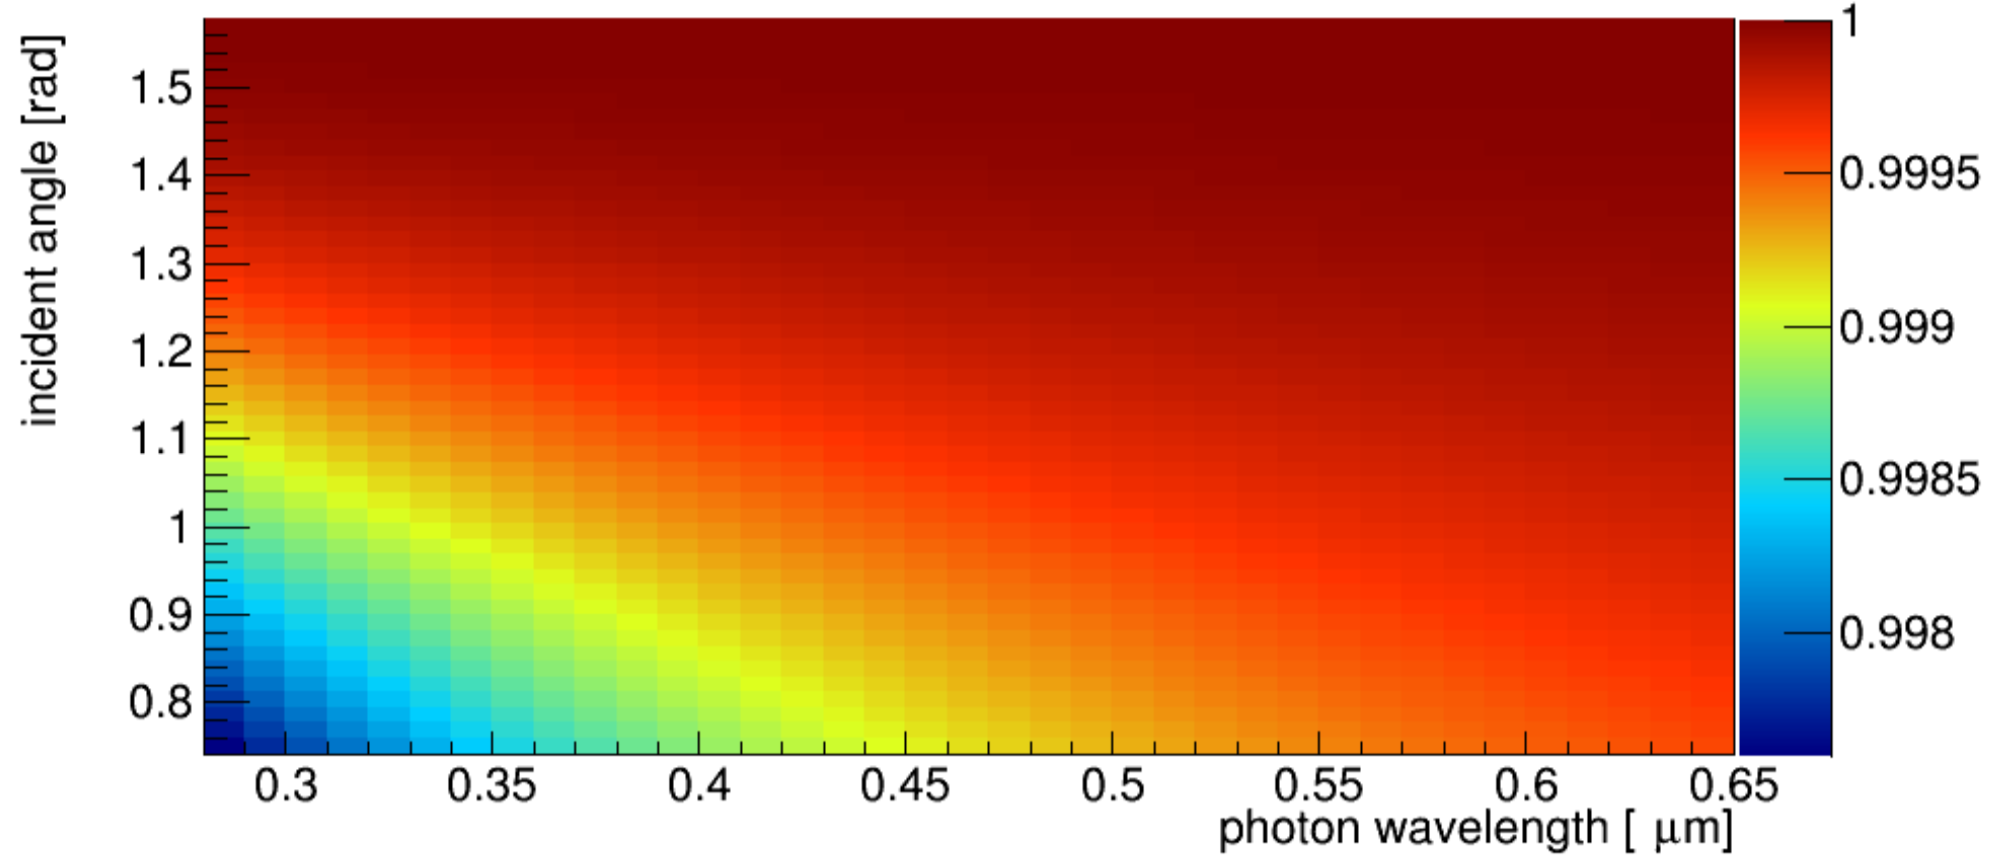
\includegraphics[width=0.95\textwidth]{pics/psurf.png}
\caption{\label{pic:sur}
Reflection coefficient $P$ as a function of the wavelength and incident angle of the Cherenkov photon.
}
\end{figure}

\begin{figure}[!h]
\centering
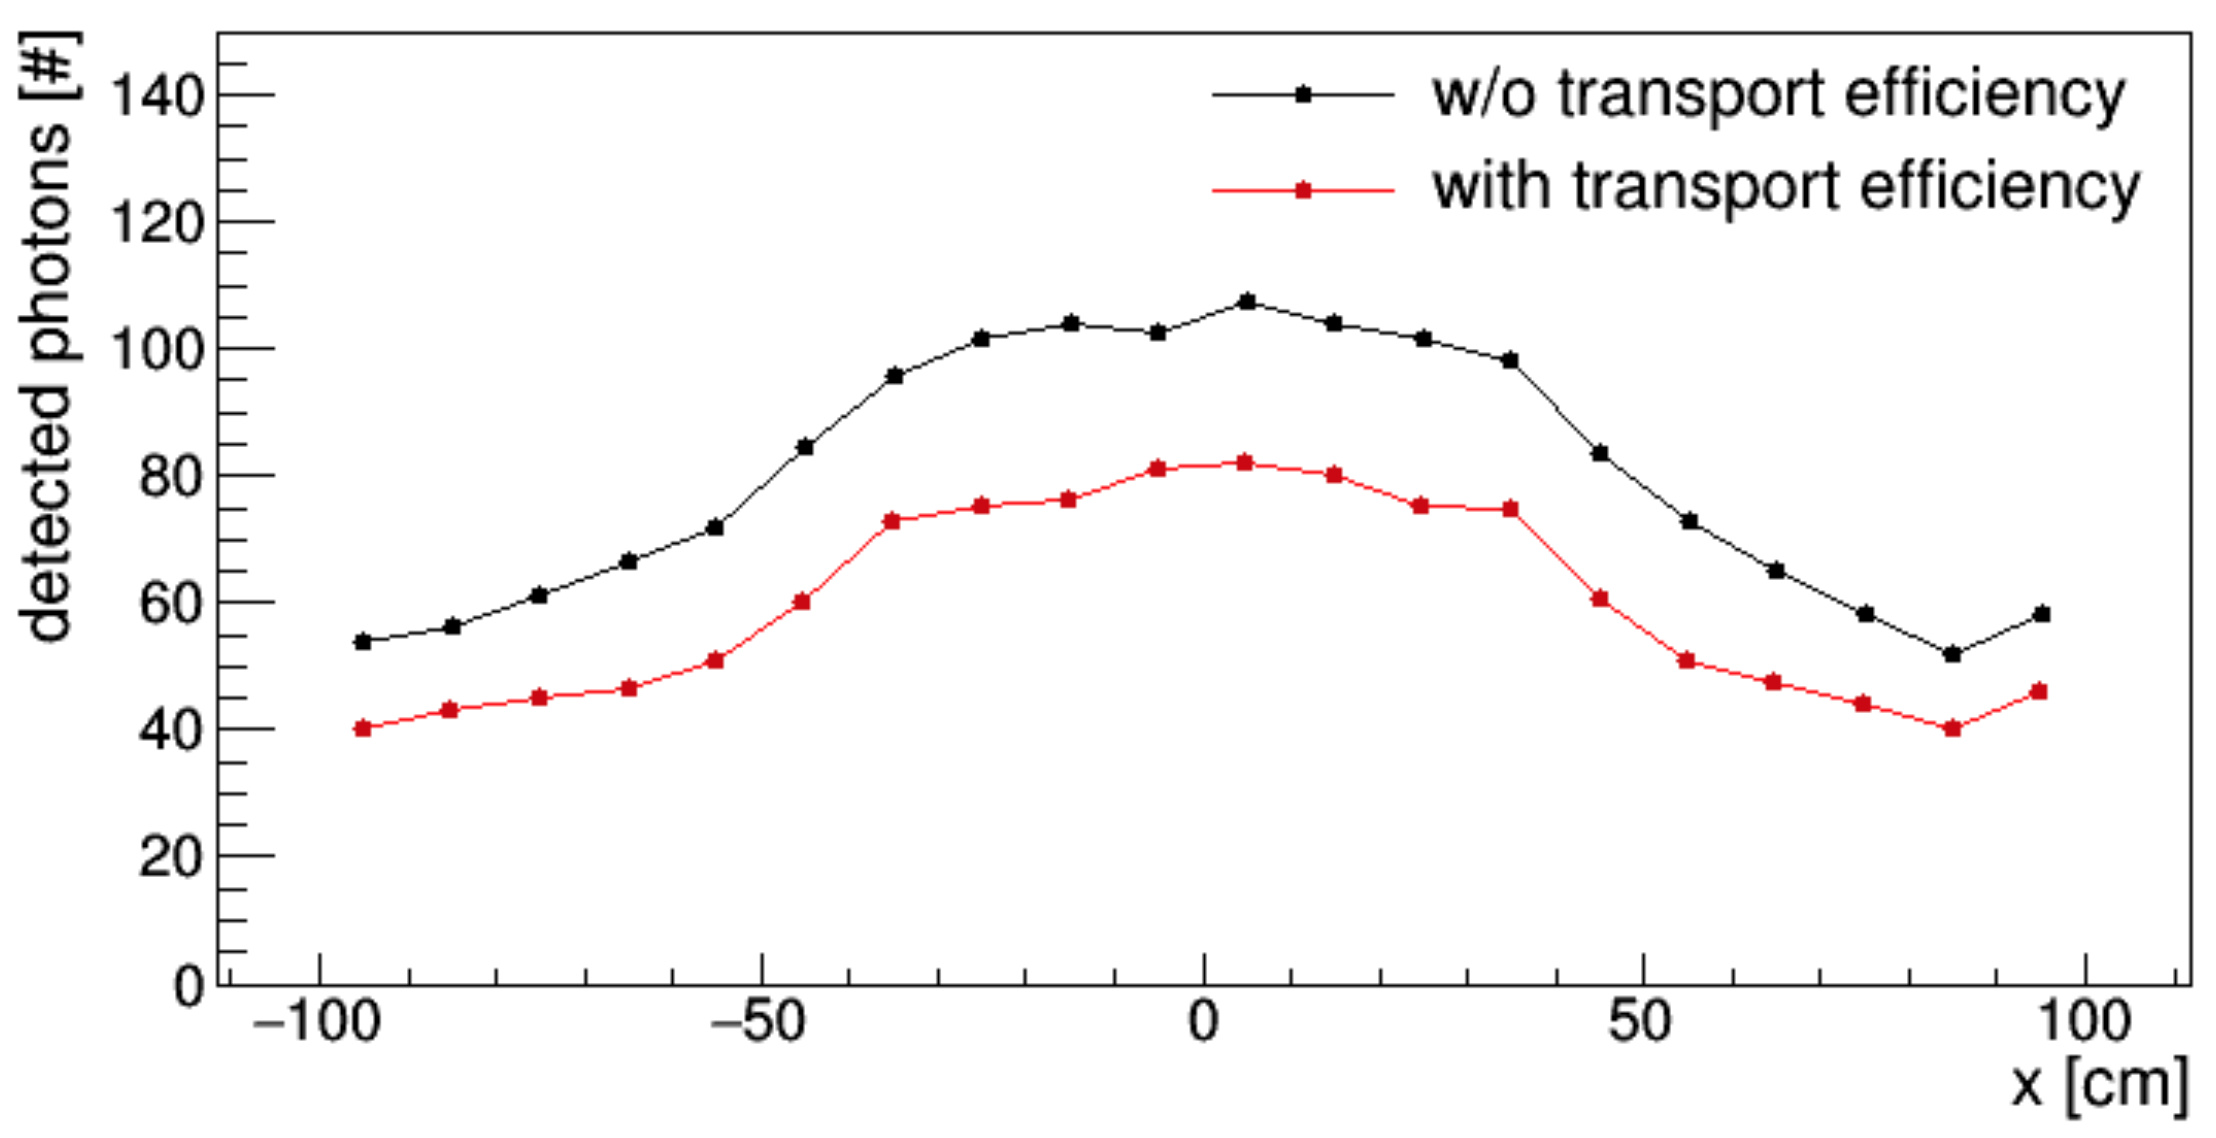
\includegraphics[width=0.8\textwidth]{pics/transport.png}
\caption{\label{pic:tra}
Impact of the transport efficiency on the photon yield. The study is based on $100k$ of $h'(2600)$ events. The photon yield is shown for the bar closest to the beamline (bar number 24 or 0 in Fig.~\ref{pic:dircNumb}).
}
\end{figure}

$P(\lambda,\alpha)$ is illustrated in Fig.~\ref{pic:sur}. The probability to survive the transpotation through the radiator can be calculated as $P_{total} = P^{N}$. Here $P_{total}$ is the transport efficiency for a given photon, and $N$ is the total number of reflections inside the radiator. We used experimental data of the transport efficiency, which agrees with the scalar theory for roughness value of $r \approx 5 A$~\cite{roughness}. Figure~\ref{pic:tra} illustrates the impact of the transport efficiency on the photon yield for tracks hitting the bar closest to the beamline (bar number 24 or 0 in Fig.~\ref{pic:dircNumb}) in different points along the $x$ axis. The effect is larger in the middle and decreases towards the ends of the bar. This correlates with the orientation of the Cherenkov cone inside the radiator: when a charged particle hits the middle of the bar, the axis of the Cherenkov cone is oriented almost perpendicularly to the bar, and photons have more reflections on the radiator sides than for the case when the charged particle traverses the bar at a more shallow angle.

The photon sensors are implemented in the simulation as a set of functional layers (see Fig.~\ref{pic:struct}). Propagation of Cherenkov photons through them is handled by {\geant}4. The quantum efficiency (QE) of the photosensors (see Fig.~\ref{pic:qe}), is applied at the production stage to avoid tracing photons which are not going to be detected.

\begin{figure}[!h]
\centering
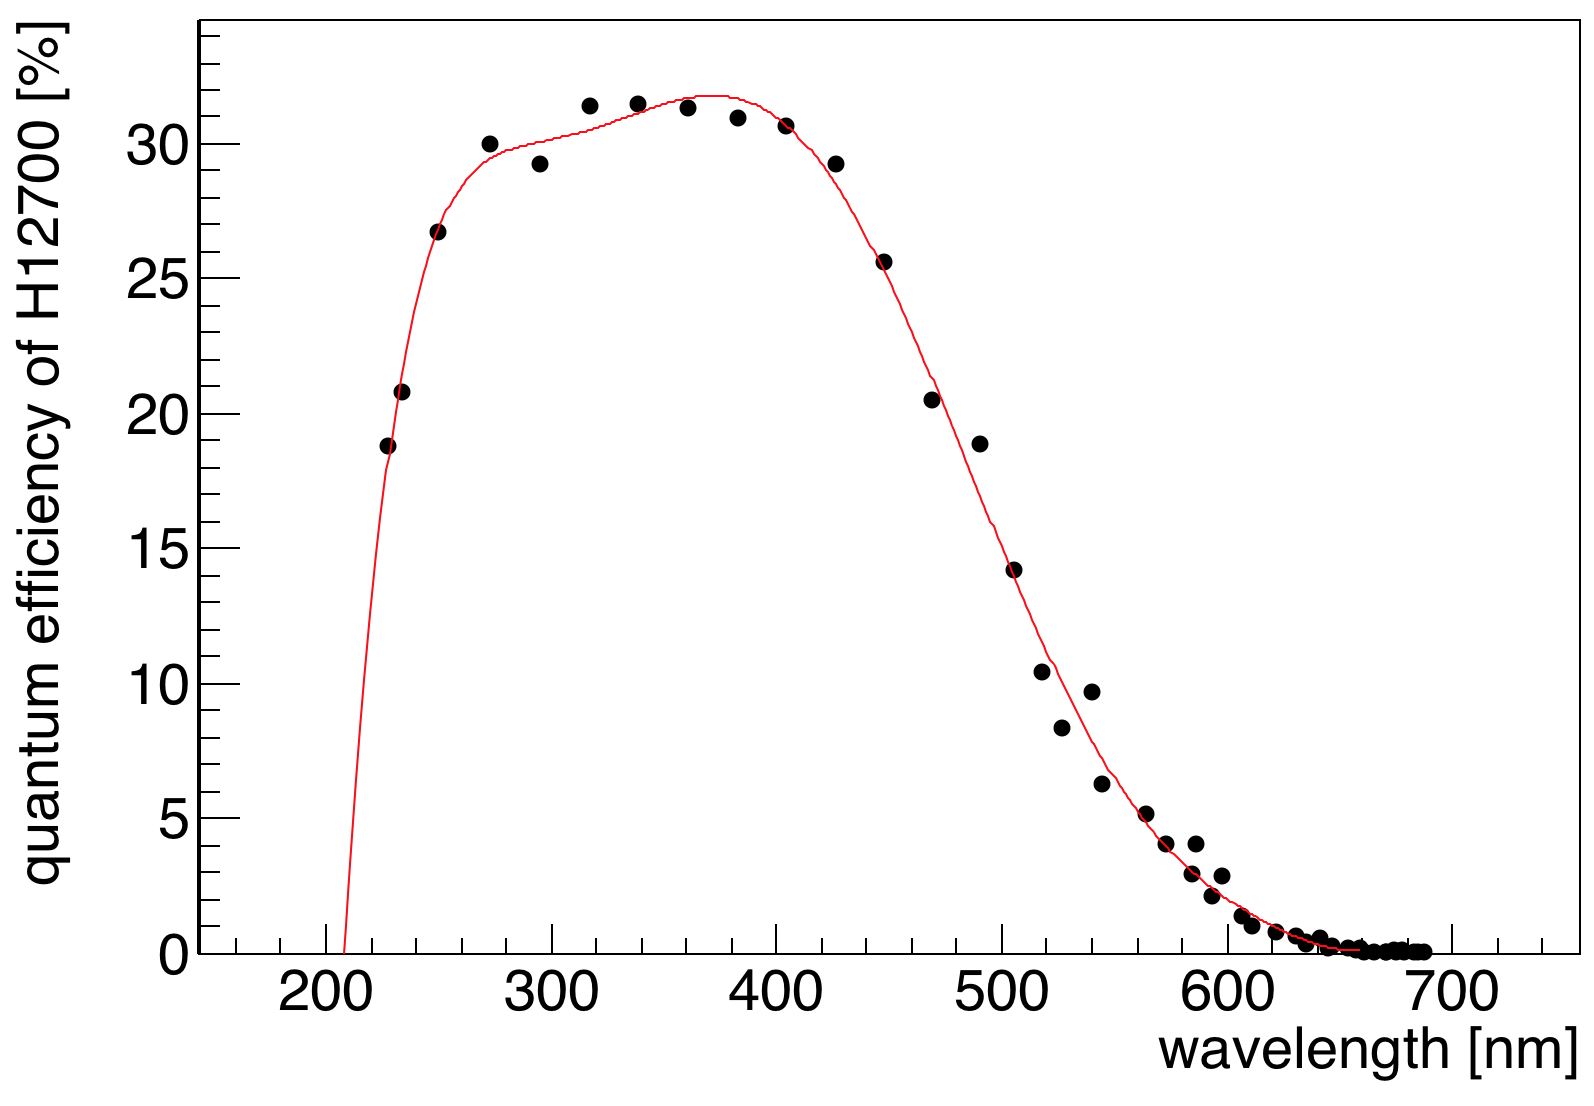
\includegraphics[width=0.6\textwidth]{pics/qe.png}
\caption{\label{pic:qe}
Quantum efficiency (QE) of photosensors Hamamatsu H12700. The red line shows a fit to the data points, extracted from the data sheet.
}
\end{figure}

\begin{figure}[!h]
\centering
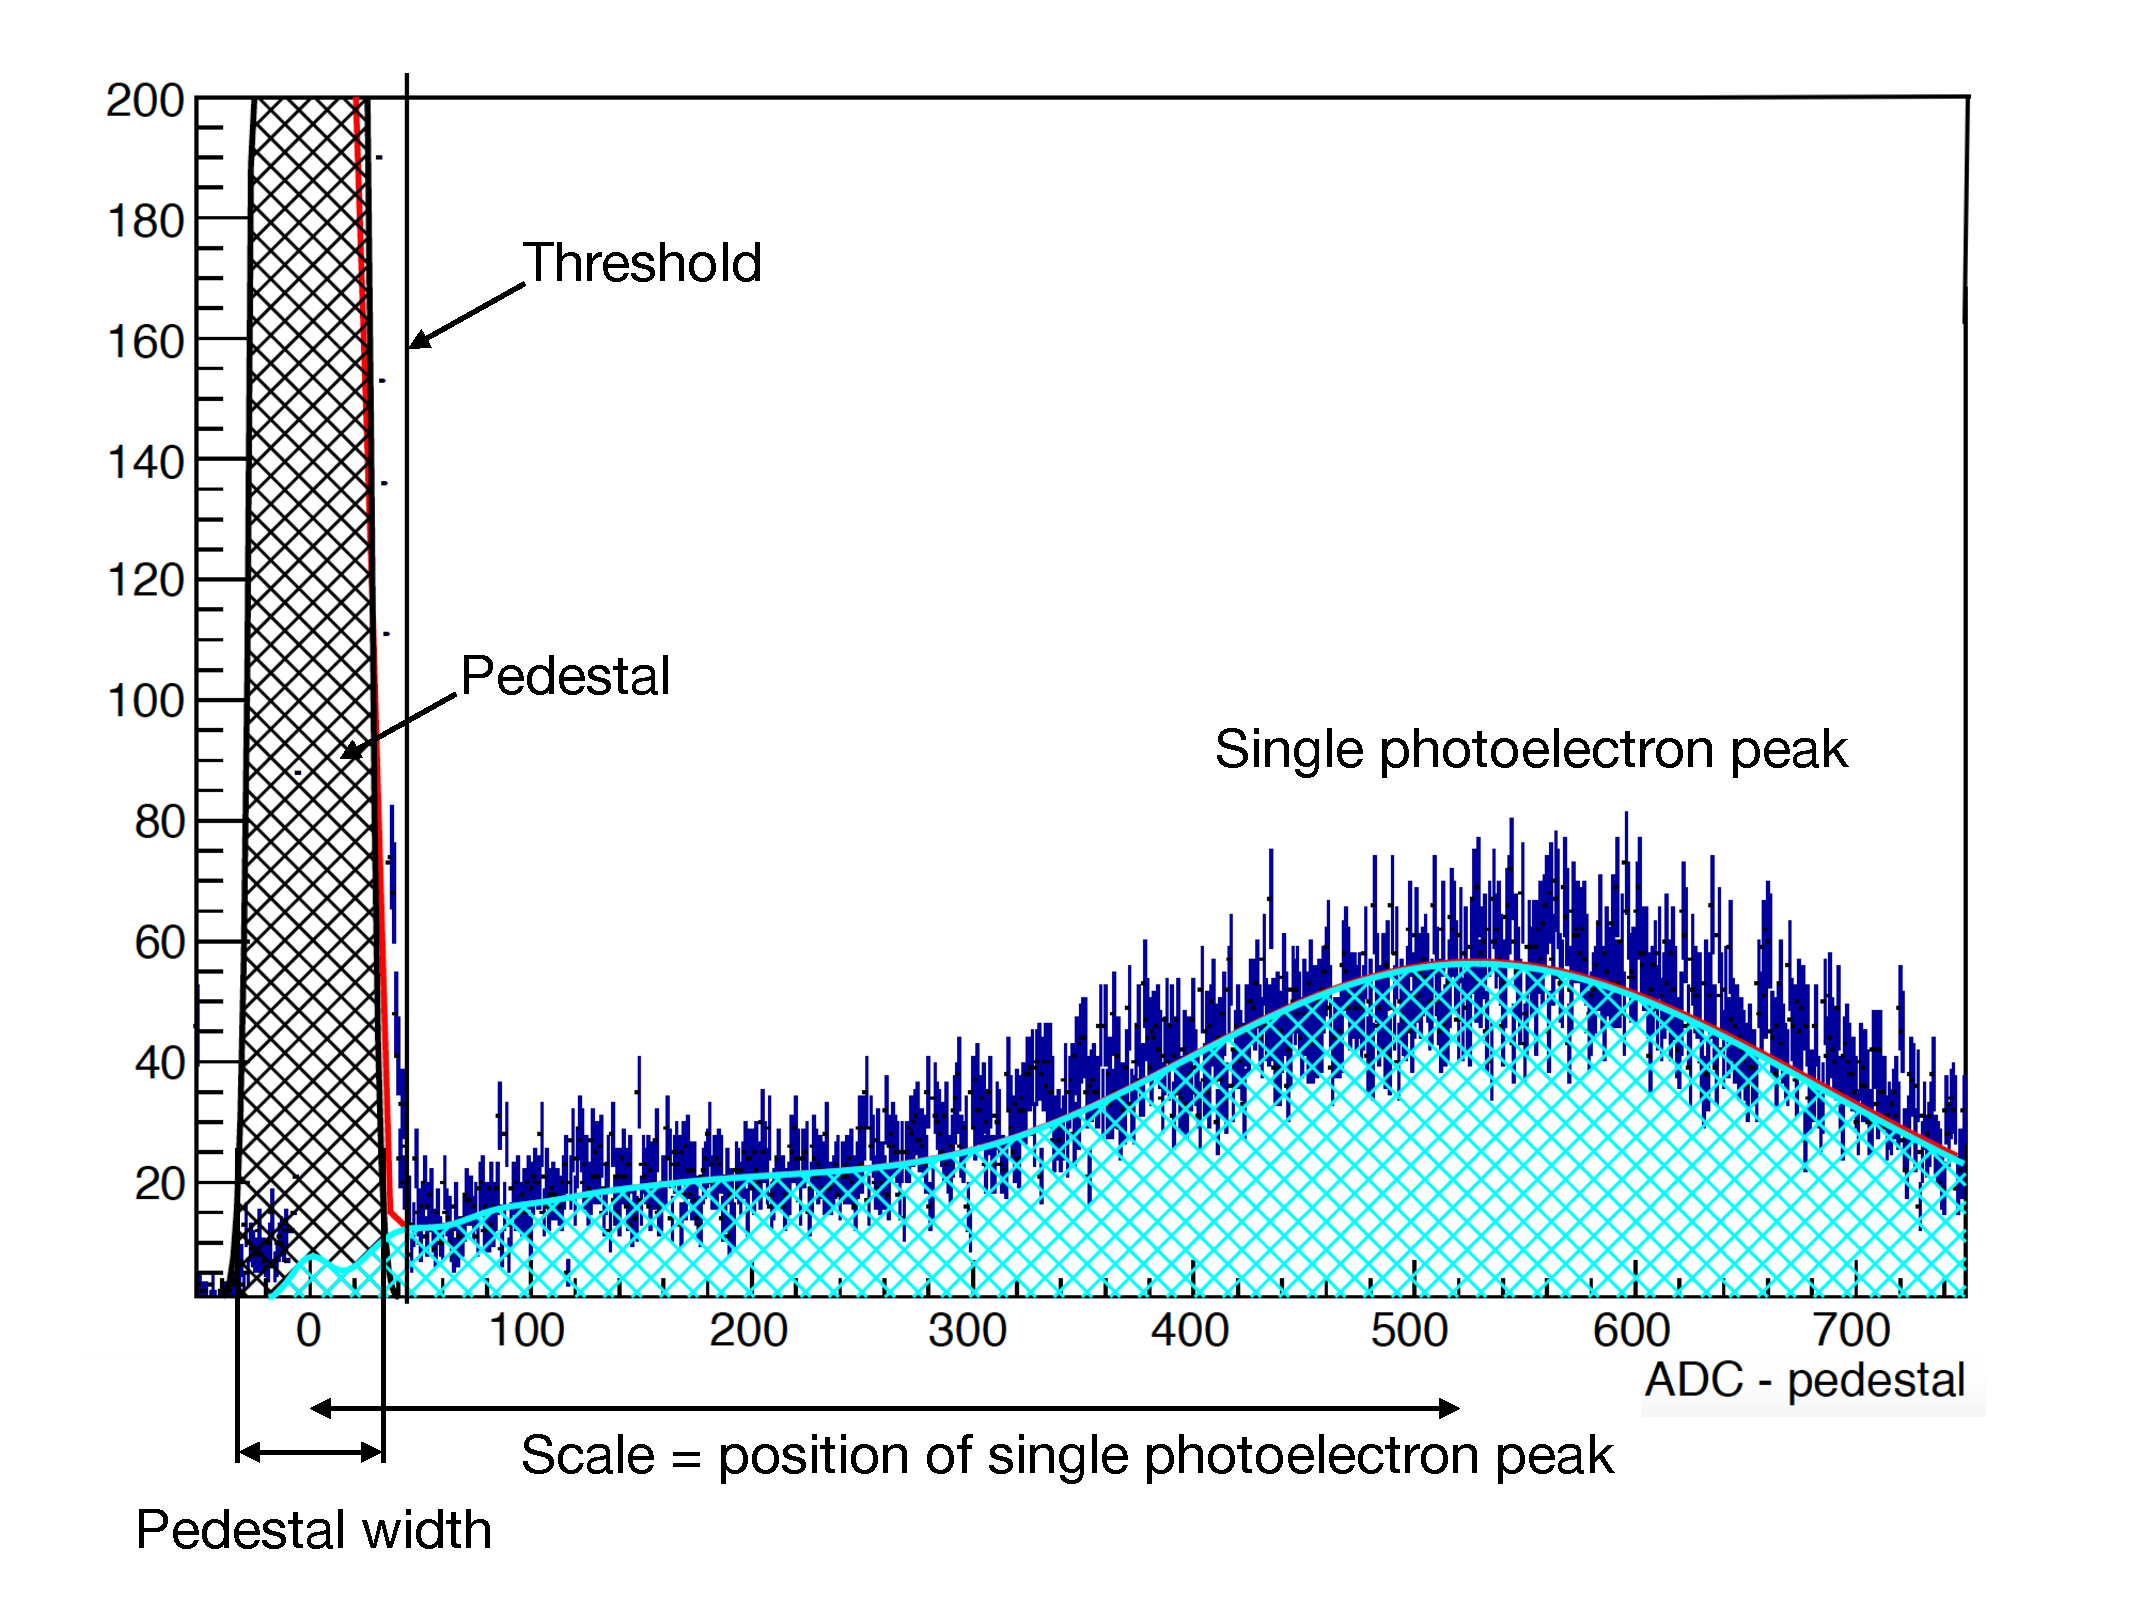
\includegraphics[width=0.65\textwidth]{pics/adc.pdf}
\caption{\label{pic:adc}
An example of the ADC spectrum for a MaPMT pixel. The pedestal is centered at 0. The fit for the single photoelectron peak, based on~\cite{deg}, is shown in cyan.
}
\end{figure}

The ADC spectra for all MaPMT were measured individually using a laser setup with the wavelength of 400 nm to derive the pixel-by-pixel efficiency $\epsilon_{400}$. An example of the ADC spectrum is shown in Fig.~\ref{pic:adc} (here the pedestal mean is put in 0). The ADC spectra were fitted according to~\cite{deg}. The width and position of the pedestal, as well as the position of the single photoelectron peak vary between pixels (see Fig.~\ref{pic:effi}a,c,d). Alignment of single photoelectron peaks between different pixels by setting a corresponding amplifications (scale factors) allows to use the same threshold value for all MaPMTs. The pixel-by-pixel efficiency $\epsilon_{400}$ was calculated as the number of photons in the single photoelectron peak divided by the number of incident photons, which is known from the laser settings. Figure~\ref{pic:effi}b shows $\epsilon_{400}$ for all pixels: the distribution is peaking around the mean value, which can be chosen arbitrarily. The pixel-by-pixel efficiency is assumed to be independent on the wavelength, so that  the total detection efficiency is $\epsilon_{400} \times$ QE (see Fig.~\ref{pic:qe}). To add the effect of $\epsilon_{400}$ at the mcsmear stage one needs to forsee the possibility to increase the total efficiency (as $\epsilon_{400}$ can be > 1). For that QE is scaled  by 2 and the mean value of $\epsilon_{400}$ is set to 0.5. The values for individual pixels for $\epsilon_{400}$ are read out from ccdb.

\begin{figure}[!h]
\centering
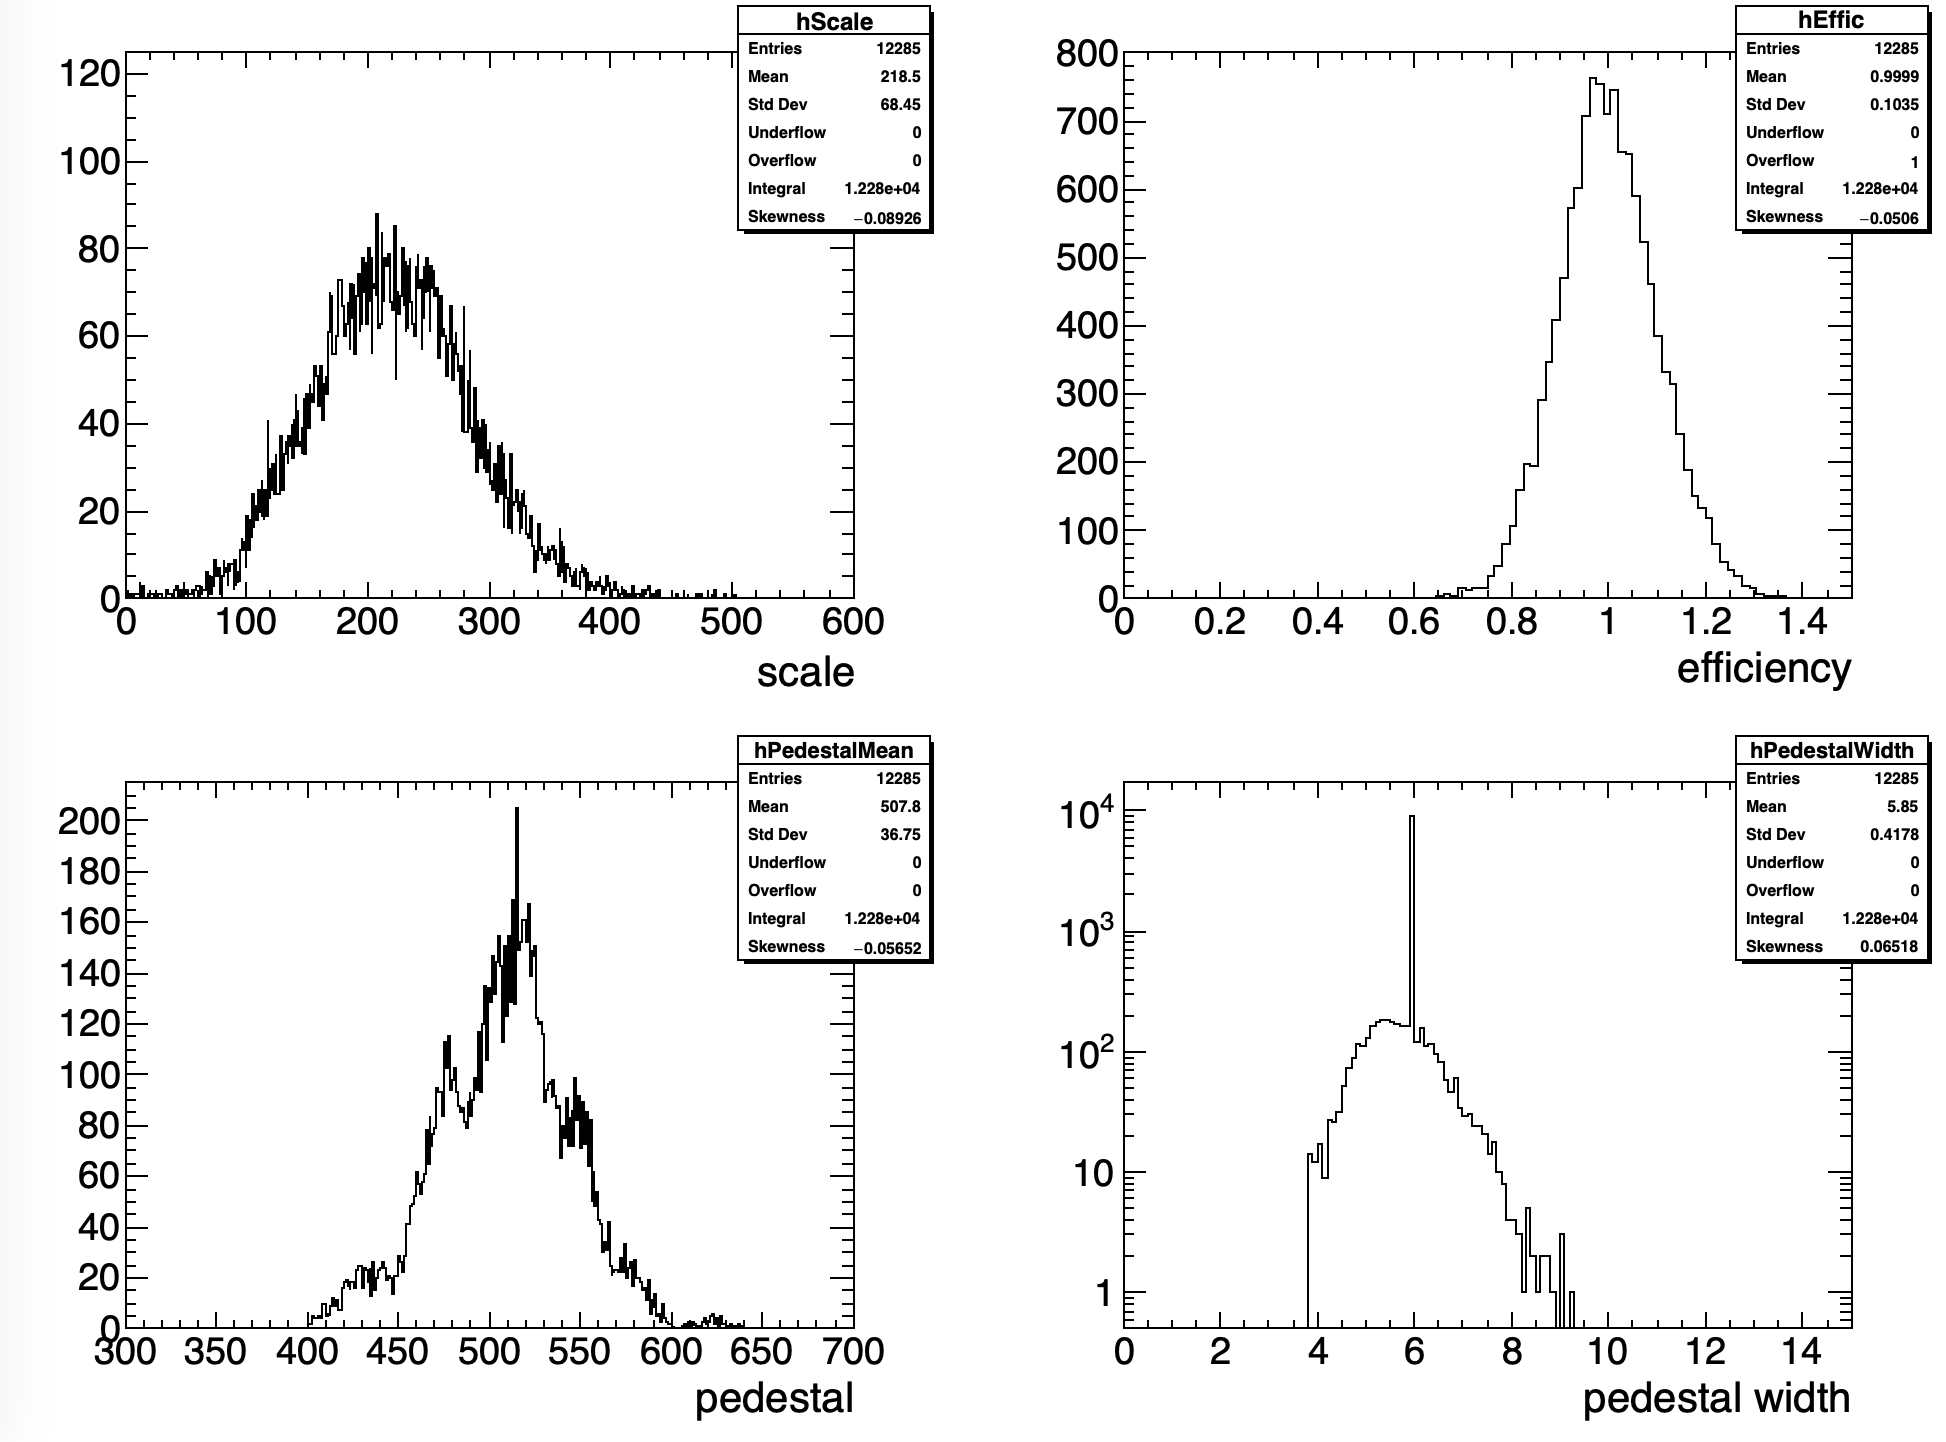
\includegraphics[width=0.9\textwidth]{pics/effi.png} \put(-320,230){a)} \put(-320,100){c)} \put(-130,230){b)} \put(-130,100){d)}
\caption{\label{pic:effi}
ADC spectrum fitting parameters plotted for all pixels: a) scale, which is the location of the single photoelectron peak in ADC counts, b) efficiency of a single pixel, c) pedestal mean value in ADC counts, d) pedestal width in ADC counts.
}
\end{figure}

The deterioration effects caused by imperfections of the physical shape of the radiators are not taken into account. The radiator bars in the detector simulation are perfect parallelepipeds, unlike in reality. Therefore, systematic smearing of the photon direction at every reflection inside the real radiator, which introduces an additional error to the reconstructed photon direction and therefore, to the obtained Cherenkov angle, is not (yet) taken into account.


\subsection{Material properties}

The nessesary Cherenkov properties of materials include refraction index and absorption lenght for a range of photon energies (see \texttt{hdds/Material{\_}HDDS.xml}). The materials coupling together the elements of the detector optical system can introduce additional photon losses due to their poor Cherenkov properties. 

The following table summarizes the sources for the material properties used in the simulation. The refraction index data was taken from (or compared to) (*) \\ \url{https://refractiveindex.info}. 

\vspace{0.5cm}
\begin{tabular}{| c | c | c |}
\hline
\textit{material} & \textit{refraction index} & \textit{absorption length} \\
\hline
Fused Silica & * & \cite{Epotek} \\
\hline
Water & * and~\cite{EpotekData} & based on~\cite{water} and~\cite{water2} \\
\hline
Epotek 301-2 & \cite{EpotekData} & \cite{Epotek} \\
\hline
cathode & $n = 2.7$ & $0.0001$ to stop photons \\
\hline
PMT window & * &  from Borosilicate Crown data sheet \\
\hline
RTV615 & $n = 1.406$ & our measurements \\
\hline
OCF 446 & $n = 1.46$ & copied from RTV615 \\
\hline
Optical air\footnote{In the simulation the bars are surrounded by air and not by nitrogen, as in reality.} & $n = 1$ & $100$ m, constant \\
\hline
\end{tabular}
\vspace{0.5cm}

Figures~\ref{pic:mat1} and~\ref{pic:mat2} show the refraction indices and absorption lengths for the materials used as a function of photon wavelength and energy.

\begin{figure}[!h]
\centering
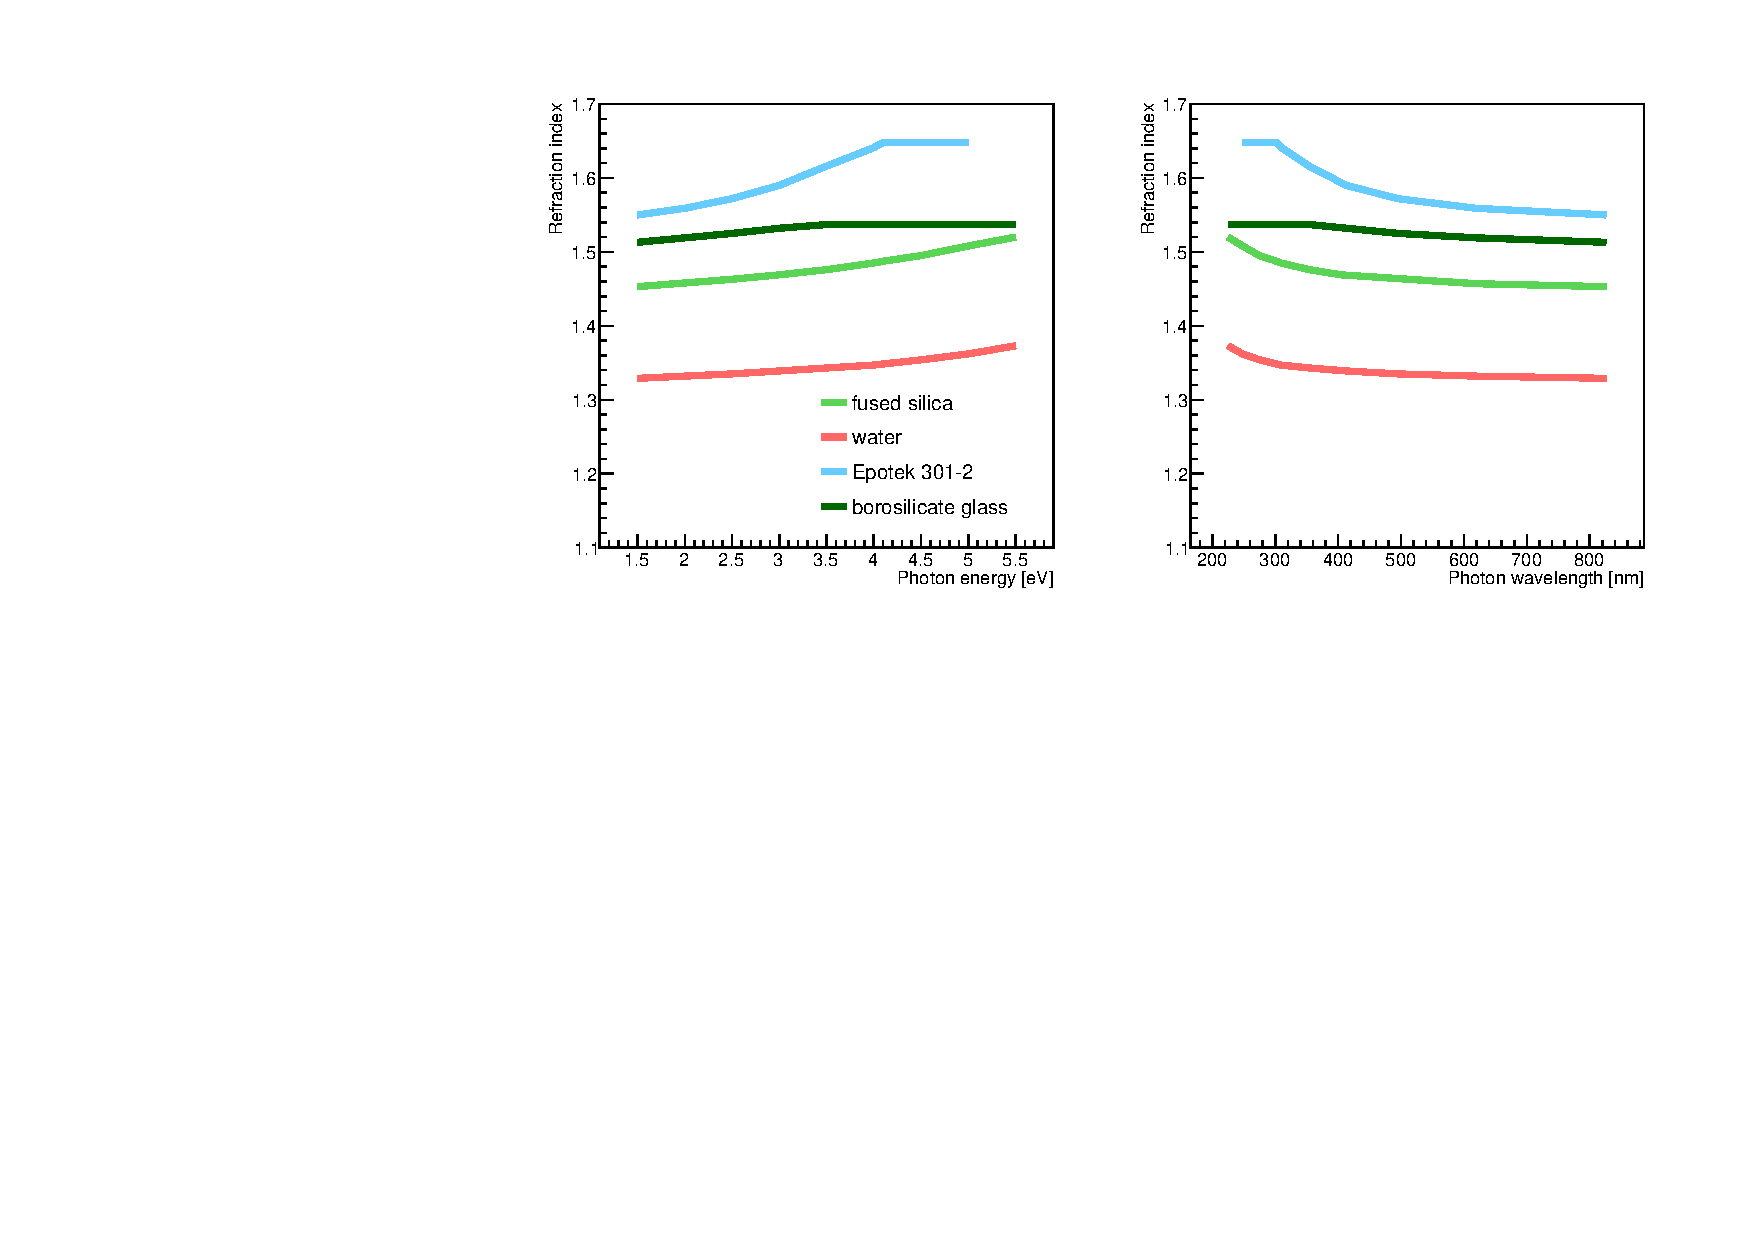
\includegraphics[angle=0,width=0.95\textwidth]{pics/refind1.pdf}
\caption{\label{pic:mat1}
Refraction index as a function of the photon energy (left) and wavelength (right) for the materials used in the simulation.
}
\end{figure}

\begin{figure}[!h]
\centering
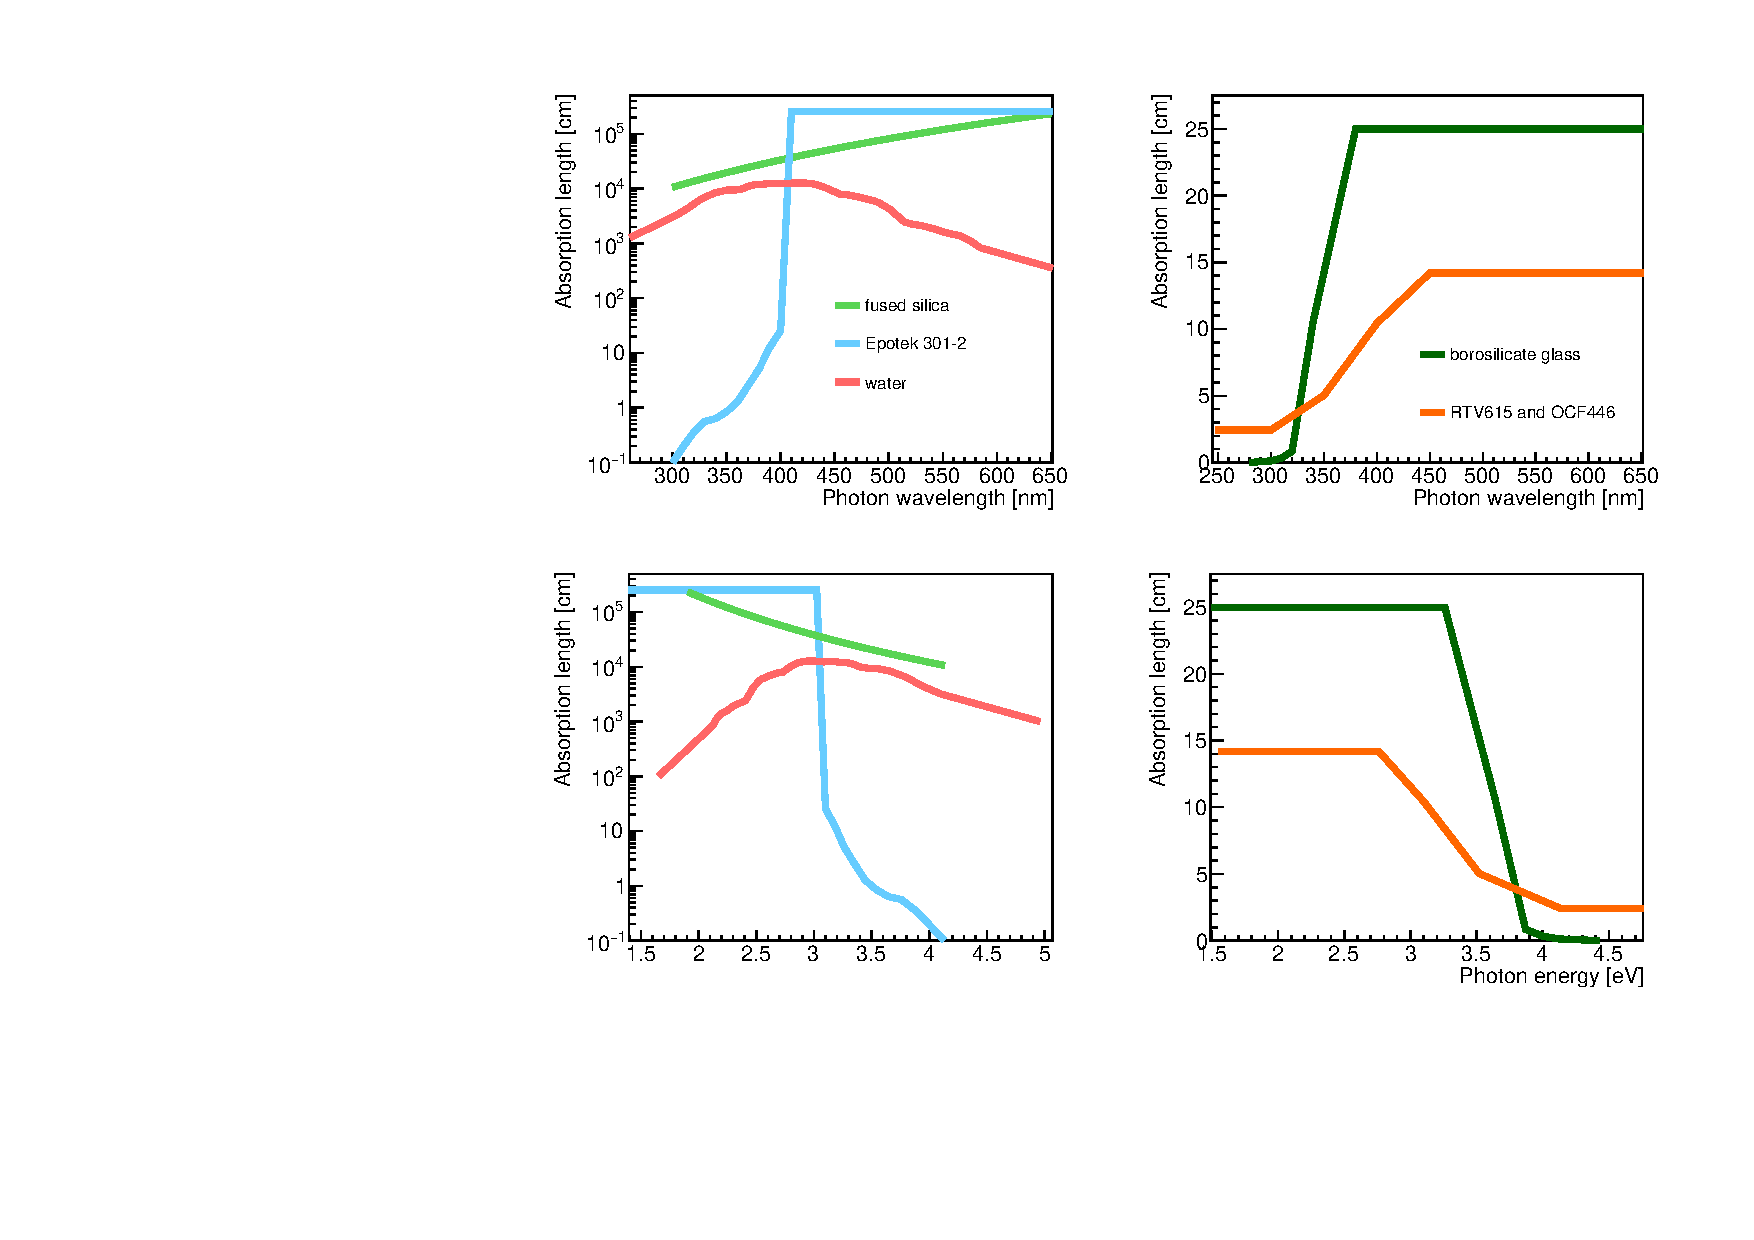
\includegraphics[angle=0,width=0.95\textwidth]{pics/ablen1.pdf}
\caption{\label{pic:mat2}
Absorption length as a function of the photon energy (left) and wavelength (right) for the materials used in the simulation.
}
\end{figure}

\subsubsection*{Epotek 301-2 optical glue}

The \babar DIRC radiators are glued out of four pieces (see Fig.~\ref{pic:bar}) using Epotek $301-2$~\cite{Epotek} optical glue. The nominal thickness of the glue layer is $d_{glue} = 50 \mu m$. The same glue was used to attach the small wedge and the bar box window. The refraction index for Epotek 301-2 was taken from~\cite{EpotekData}. The absorption length was adopted from~\cite{EpotekData}.

\subsubsection*{Borosilicate glass}

H12700 PMTs can have either borosilicate glass or UV glass. The \gluex DIRC uses H12700 with borosilicate glass. The nominal thickness of the PMT window is $1.5$ mm (see spec sheet). The absorption length from the Schott Borosilicate Crown Glass data sheet is shown in Fig.~\ref{pic:gla}. The transmittance values should be corrected for Fresnel reflection. Fresnel reflection of the air-glass interface can be calculated as:

\begin{equation}
R = \Bigl( \frac{n_1 - n_2}{n_1 + n_2} \Bigr)^{2} = \Bigl( \frac{1.53 - 1}{1.53 + 1} \Bigr) ^{2} \approx 4.4\%,
\label{eq:fre}
\end{equation}

\noindent where $n_1 = 1.53$ is the refraction index for borosilicate glass, $n_2 = 1$ -- refraction index for air. The light passed the following tnerfaces: air-glass, glass-air. On each of two interfaces the Fresnel reflection should be taken into account leading to $R_{total} = 8.6\%$. The incident light was partly reflected ($R_{total}$), partly absorbed ($A$), and partly transmitted ($T$): $ R_{total} + T + A = 1$. For the absorption length $\lambda$ we need $1 - A = R_{total} + T = e^{-x/\lambda}$. 

\begin{figure}[htb]
\centering
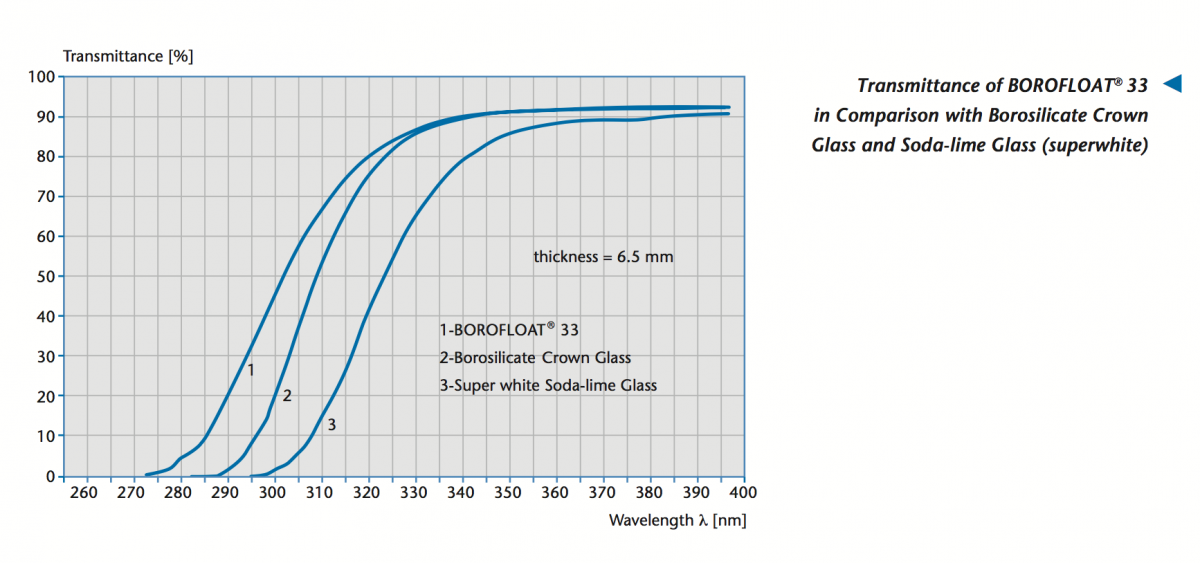
\includegraphics[angle=0,width=0.8\textwidth]{pics/glass.png}
\caption{\label{pic:gla}
Transmittance for the borosilicate glass~\cite{borospec}.
}
\end{figure}

\begin{equation}
\lambda = -x/\log(R_{total}+T) = -0.15/\log(0.086+T),
\label{eq:lam}
\end{equation}

\noindent here we assume glass thickness $x = 0.15$ cm. The following table shows absorption length for the borosilicate glass extracted from the Fig.~\ref{pic:gla} plot (line 2):

\begin{center}
\begin{tabular}{| c | c | c | c | c | c | c | c |}
\hline
wavelength [nm] & 280 & 300 & 310 & 320 & 340 & 380 \\
\hline
transmittance & 0 & 0.20 & 0.55 & 0.75 & 0.90 & 0.92 \\
\hline
$\lambda$ [cm] & 0 & 0.12 & 0.33 & 0.84 & 10.6 & 25.0 \\
\hline
\end{tabular}
\end{center}

\subsubsection*{Silicone cookies}

The material used to produce cookies is RTV615 by Momentive. The mixing ratio is $100 : 2.5$ (unlike the default mixing ratio of $10 : 1$), which makes the pad softer. The average thickness of the real cookies is $0.17$ cm, and the area is $5.2$ cm times $15.8$ cm. For the simulation the refraction index of the cookies is set constant $n = 1.406$, and the absorption length is taken from our measurements (see Fig.~\ref{pic:coo}). All the custom-made cookies have similar and good transmittance properties independently on the curing method or mixing ratio.

\begin{figure}[!tb]
\centering
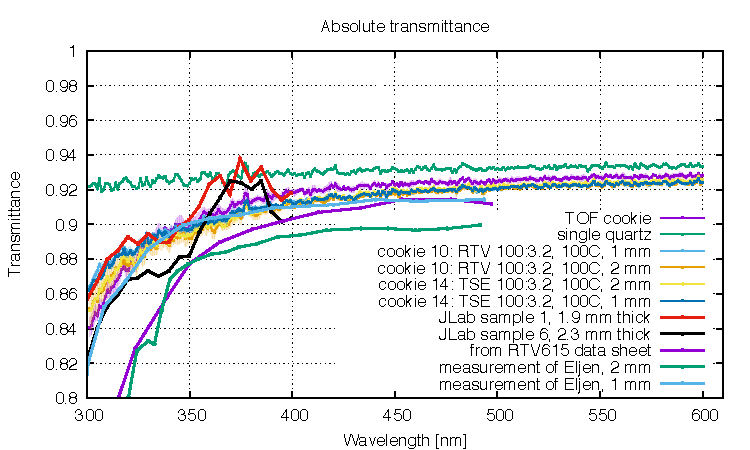
\includegraphics[angle=0,width=0.9\textwidth]{pics/transmittance1.pdf} \\
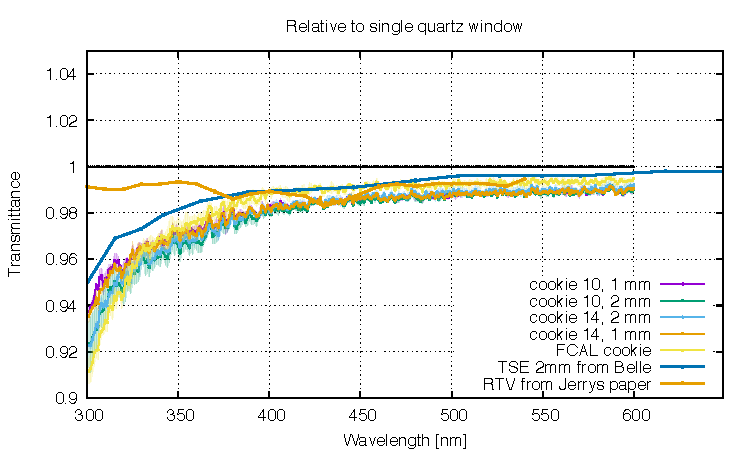
\includegraphics[angle=0,width=0.9\textwidth]{pics/cookie10_relQuartz.pdf}
\caption{\label{pic:coo}
Transmittance measurements for a set of custom-made silicone cookies. Absolute values (top), and relative to a single quartz window  (bottom). FCAL cookie is a pre-made cookie by Momentive (same RTV615 material, thickness $2$ mm). The data for TSE 2 mm cookie is taken from a plot on Belle II TOP cookies transmittance, which had poor resolution. The paper mentioned here is~\cite{slacpub}.
}
\end{figure}

The absorption length of the silicone was extracted from the absolute transmittance measurements (see Fig.~\ref{pic:coo} (top)). Transmittance was measured for the cookie sandwiched between two fused silica windows. Fresnel reflection of the air-fused silica interface can be calculated similarly to~(\ref{eq:fre}) using $n_1 = 1.47$, the average refraction index for fused silica, leading to $R = 3.6 \%$. The total reflection loss for a single quartz window in air is then $R_{total} = 7.1 \%$. This estimation agrees with the absolute transmittance of quartz shown in Fig.~\ref{pic:coo} above (we can neglect the absorption inside the FS window). The absorption length for the silicone cookie can be calculated using~(\ref{eq:lam}), and we neglect the Fresnel reflections on the FS-cookie interface, which is about $R = 0.05 \%$.

The following table shows absorption length for the silicone extracted from the Fig.~\ref{pic:coo} plot:


\begin{center}
\begin{tabular}{| c | c | c | c | c | c|}
\hline
wavelength [nm] & 300 & 350 & 400 & 450 & 600 \\
\hline
transmittance & 0.85 & 0.89 & 0.91 & 0.915 & 0.915 \\
\hline
$\lambda$ [cm] & 2.43 & 5.03 & 10.43 & 14.2 & 14.2 \\
\hline
\end{tabular}
\end{center}

\subsubsection*{Greasing silicone fluid OCF-446}

The Nye Lubricants OCF-446 silicone fluid is used to grease the cookies and, therefore, create a good optical coupling. The usage of particularly this product was inspired by the Belle II TOP experience. To introduce this material into simulation, its molecular structure is needed. OCF-446 is a vinyl terminated (diphenylsiloxane) dimethylsiloxane copolymer commonly referred to as a Phenyl Silicone. The molecular structure of this material is shown in Fig.~\ref{pic:ocf}. The diphenylsiloxane group in this schematic is repeated $m$ times, and dimethylsiloxane group -- $n$ times. In the material table (\texttt{hdds/Materials.xml}) the number of atoms of each type in one molecule is needed. I assume that $m = n = 1$, which leads to $20$ $C$ atoms, $30$ $H$ atoms, $4$ $Si$ atoms, and $3$ $O$ atoms. The data on the refraction index of OCF-446 is poor: there is only one measurement $n = 1.46$ at $\lambda = 589.3$ nm, which corresponds to photon energy of $\approx 2$  eV. No data on absorption length is available.

\begin{figure}[htb]
\centering
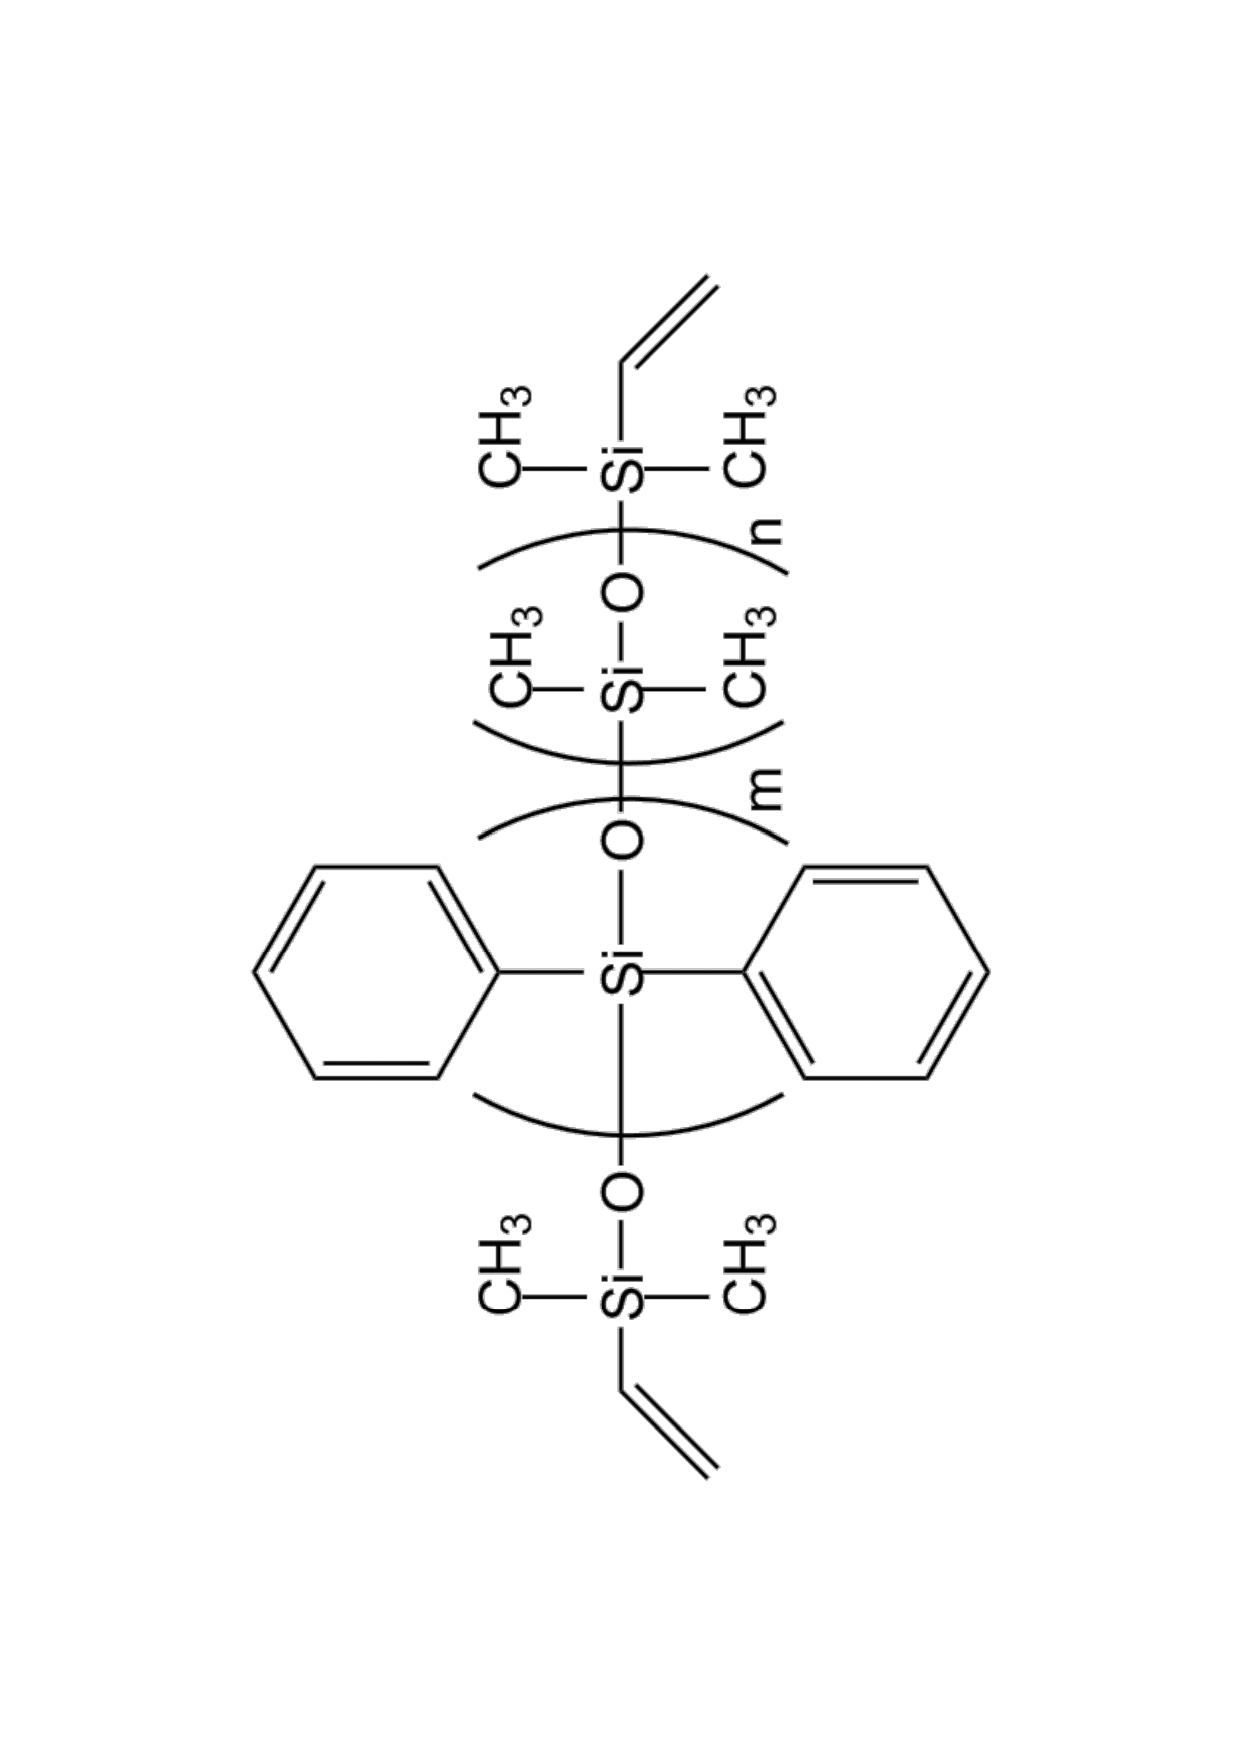
\includegraphics[angle=270,width=0.7\textwidth]{pics/ocf.pdf}
\caption{\label{pic:ocf}
A molecule of OCF-446 silicone fluid~\cite{formula}.
}
\end{figure}

There are two OCF-446 layers in the setup: one is between the PMT window and the cookie, another one is between the cookie and the window of the optical box. We can calculate the thickness of those layers based on the number of drops used. One drop is about $0.016$ g, the density of the fluid is $1.04$ g/cm$^{3}$, the cookie area is $5.2$ cm times $15.8$ cm. The assembly procedure uses $2$ drops for the layer between the PMT and the cookie. This results in an average thickness of $4 \mu m$. For the second layer the assembly procedure uses $2$ drops to grease the cookie, and another $3$ drops to put in the middle of each PMT, which results in an average layer thickness of $94 \mu m$. Both layers are introduced into the simulation, and there is no visible effect on the photon yield due to the greasing oil.

\subsubsection*{Bialkali photocathode}

According to Ref~\cite{pcpaper}, the photocathode is a thin layer of a multialkali (in our case bialkali) semiconducting alloy, which is evaporated onto the back side of the glass window during production. In the same paper we find, that it is quite difficult to extract properties of the photocathode itself. It can not be studied directly, as it is not chemically stable when exposed to air. Also, its properties might interefere with the birefringence, that is induced on the glass window by the mechanical stress due to the pressure difference (the interiour of the PMT is under vacuum). We use the simplified structure of the PMT: a borosilicate window layer followed by a layer of photocathode with the thickness of $0.1$ cm (not realistic, but it does not matter, as our photons anyways get stopped in the photocathode). 

The quantum efficiency function defines properties of the photocathode, when the light is coming from air. For the case when instead of air we have a medium with $n > 1$ (we have the fused silica window with $n = 1.47$, in~\cite{pcpaper} they use scintillator with $n = 1.48$), the authors~\cite{pcpaper} state, that the effective quantum efficiency is slightly increased compared to the one stated in the data sheet. So in the simulation we will use the data sheet quantum efficiency as a conservative estimate. We use a refraction index of $n = 2.7$ to allow {\geant}4 to perform the reflection/refraction on the PMT window -- photocathode interface. We use a photocathode absorption length of $0.0001$ cm to stop Cherenkov photons in the photocathode volume.

%{\geant}4 needs absorption length $\lambda$ as the following:

%\begin{equation}
%I = I_{0} \cdot e^{-x/\lambda},
%\end{equation}

%\noindent where $I_{0}$ is the incident intensity, $I$ -- transmitted intensity, $x$ -- thickness of the sample. Transmittance $T = I/I_{0}$ for the photocathode $T = 1 - A$, where $A$ -- absorption. In the paper~\cite{pcpaper} we see $A$ (410 nm) $= 0.44$ and $A$ (440 nm) $=0.41$, we take $A = 0.42$ and calculate $\lambda$ based on this assumption and the photocathode thickness of $x = 0.1$ cm. We get absorption length of $\lambda = 0.184$ cm. The refraction index of photocathode is $2.7$~\cite{pcpaper}. 




\subsection{DIRC signal}

\begin{figure}[!h]
\centering
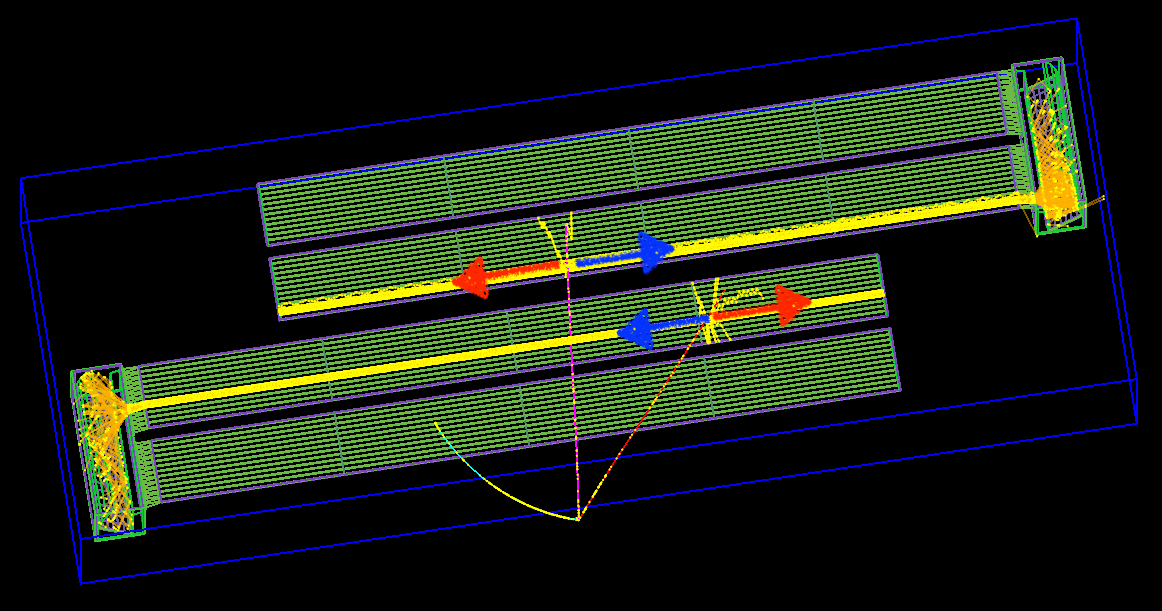
\includegraphics[width=0.75\textwidth]{pics/dir_ref.png}%eta2300decay.pdf}
\caption{\label{pic:eta2300}
An event showing the decay of $\eta(2300)$ into a kaon (red track) and a pion (magenta track). 
%A pion is shown in magenta, a kaon is shown in red. 
%A proton is shown in cyan. 
The pion and proton create Cherenkov photons (yellow tracks) inside two different DIRC radiators. The photons are transported to the optical boxes and imaged onto photodetection planes. The arrows indicate the direction of propagation for the photons going straight to the readout end of the bars (blue arrows), and photons which get reflected on the mirror at the bar end (red arrows). 
}
\end{figure}

Figure~\ref{pic:eta2300} shows a decay of $\eta(2300)$. The final state pion is shown in magenta and hits the upper bar box. The final state kaon is shown in red and hits the lower bar box. Both charged particles produce Cherenkov photons (their trajectories are shown in yellow), that propagate inside individual radiators towards the optical boxes, where they are detected. 
%An example of the single event hit pattern for a kaon and pion are shown in Fig.~\ref{pic:hitpat1} in the upper row. 

\begin{figure}[!h]
\centering
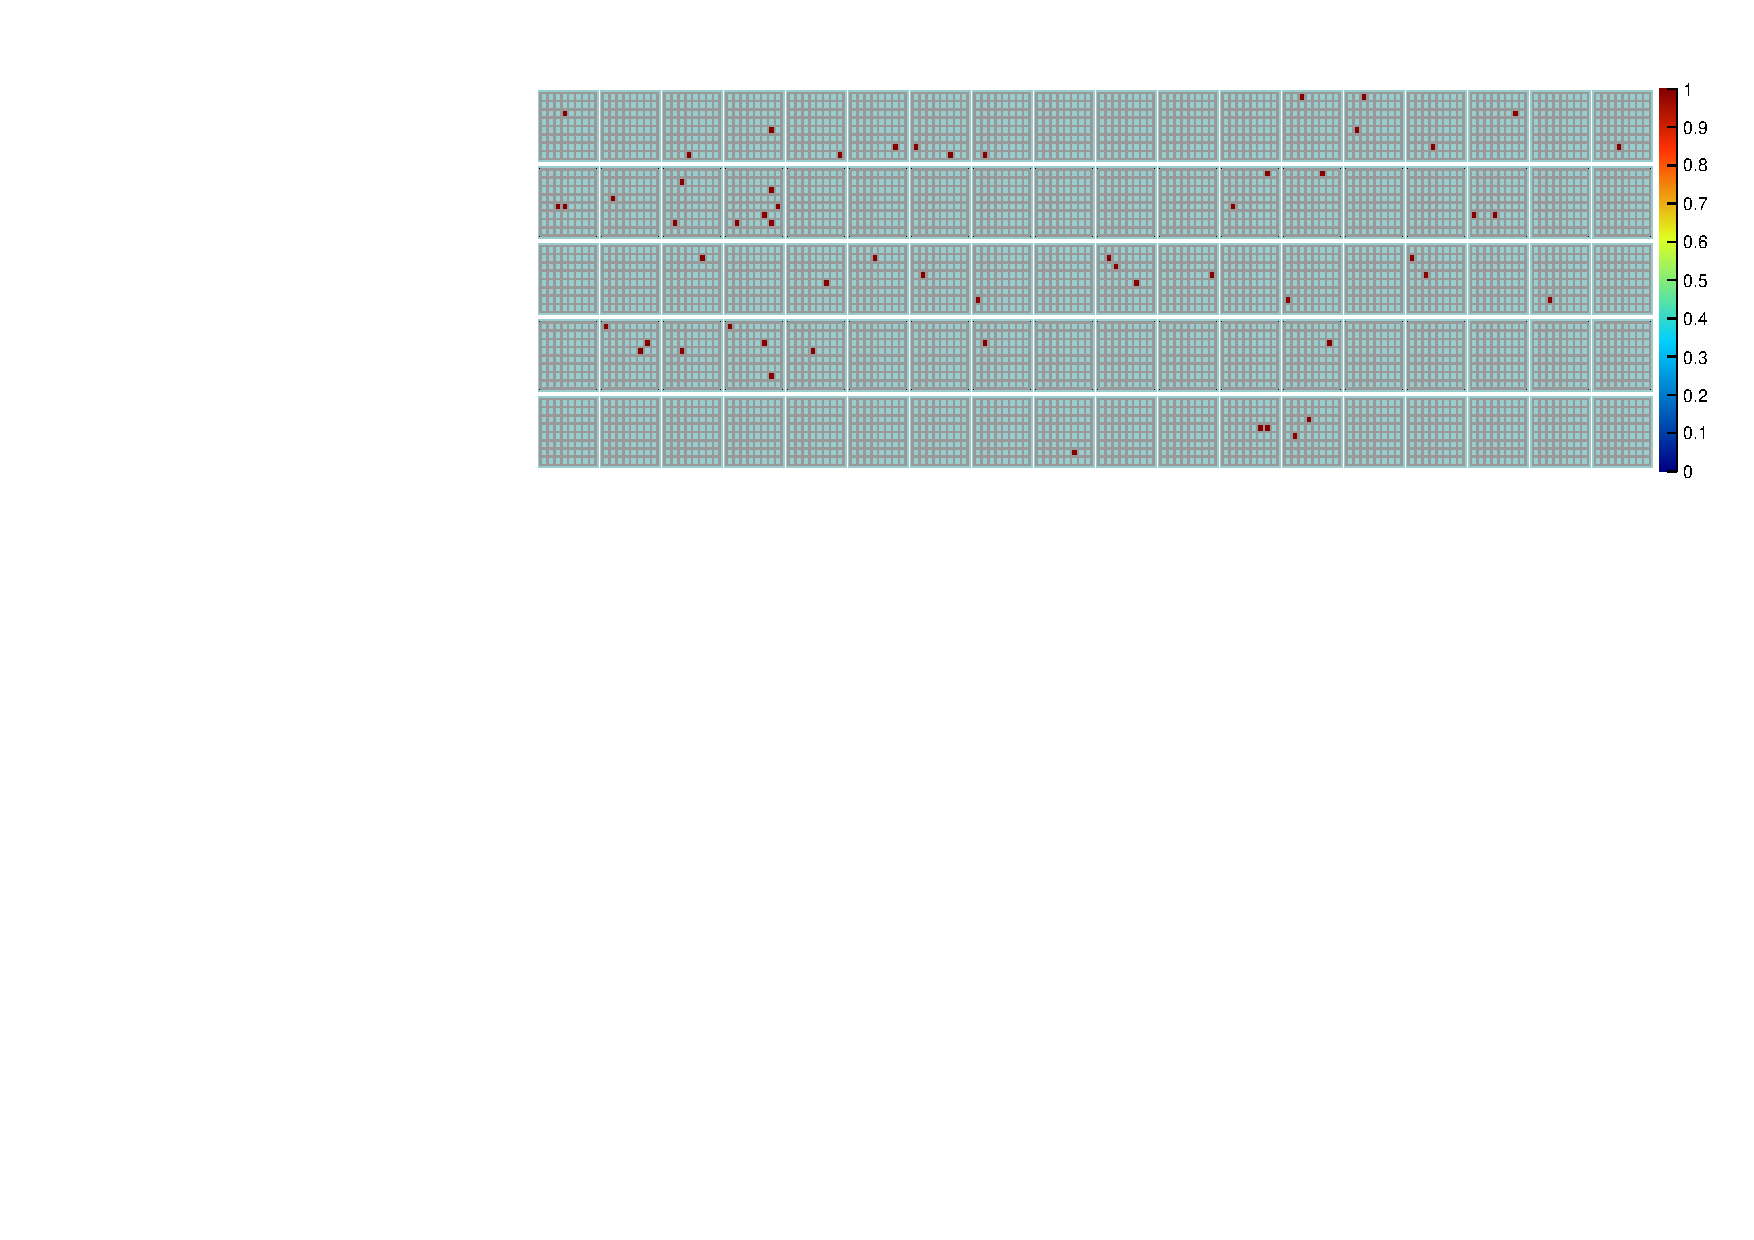
\includegraphics[angle=0,width=0.47\textwidth]{pics/kaon2GeVa.pdf} \hspace{0.5cm} 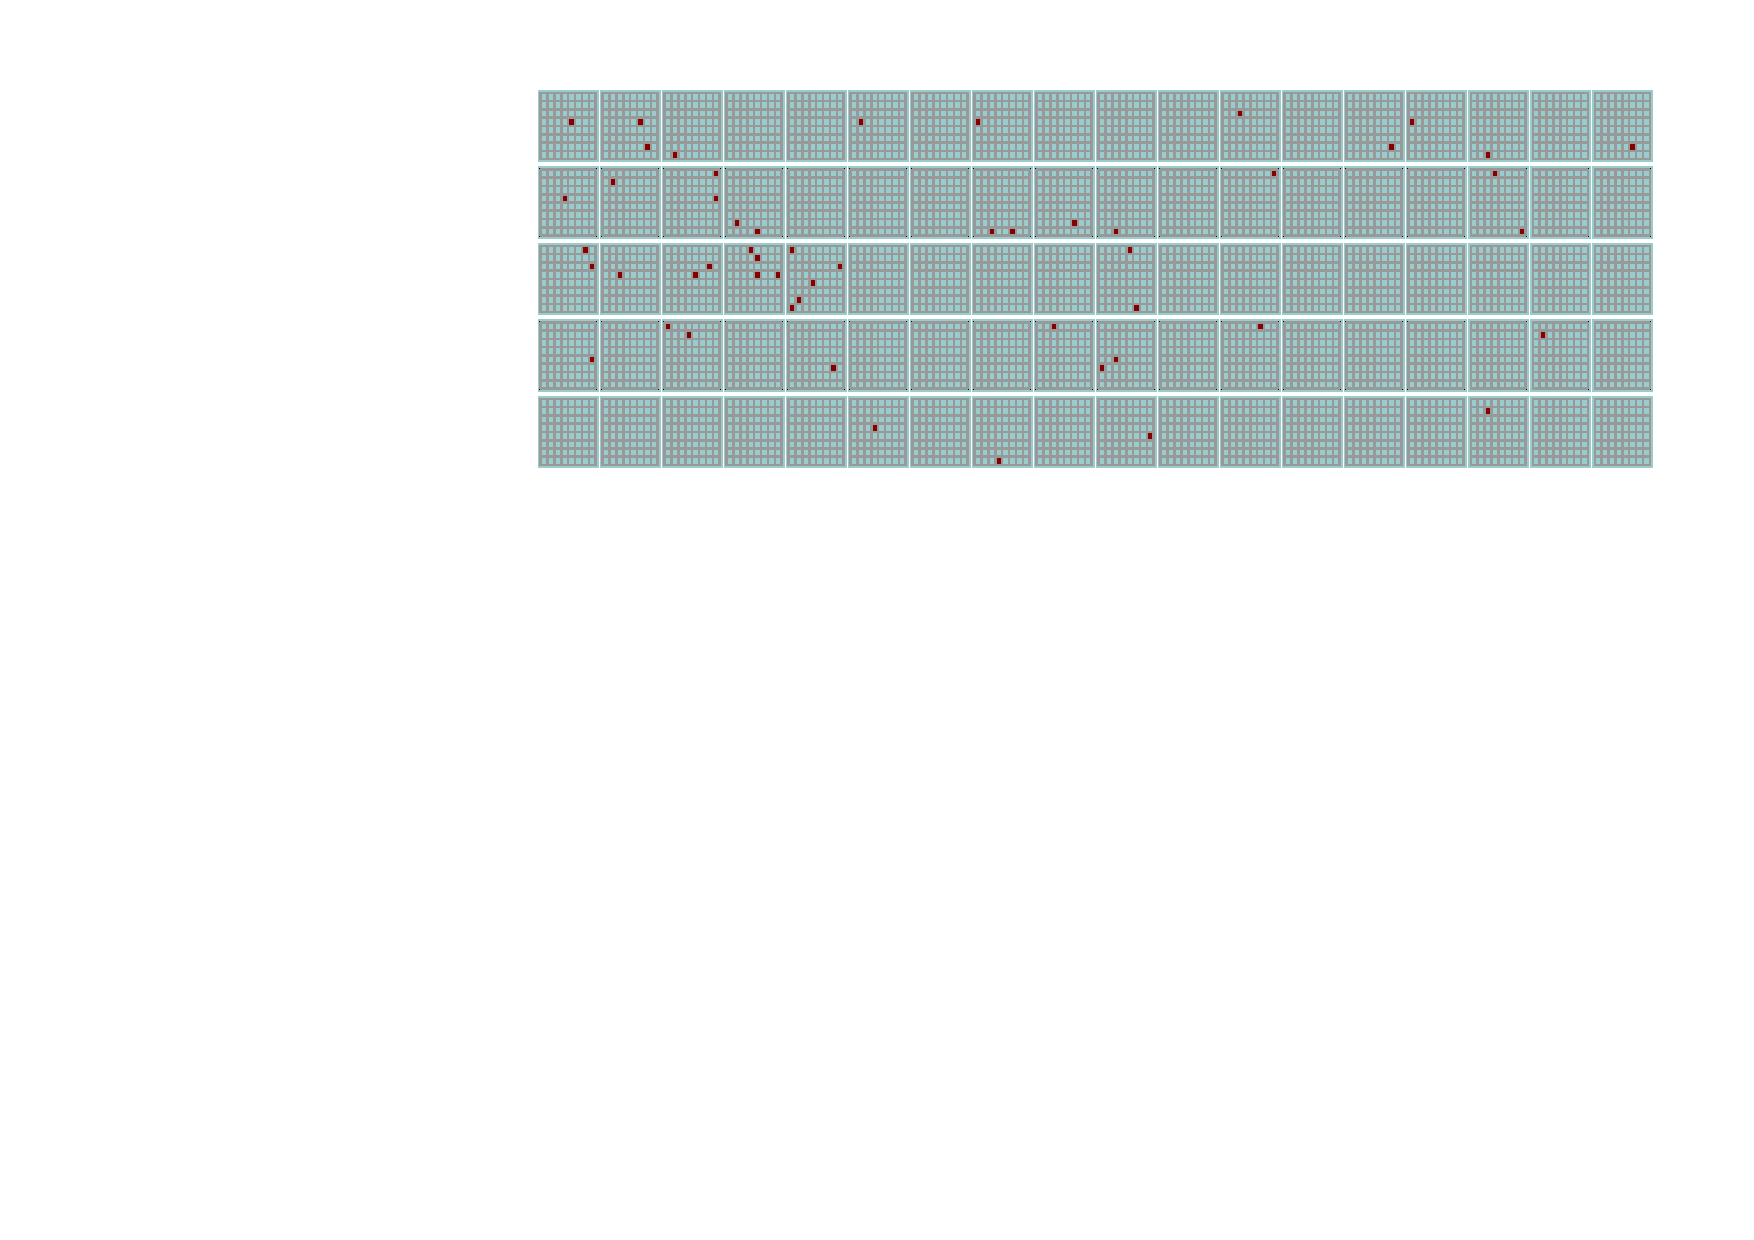
\includegraphics[angle=0,width=0.47\textwidth]{pics/pion2GeVa.pdf}\\
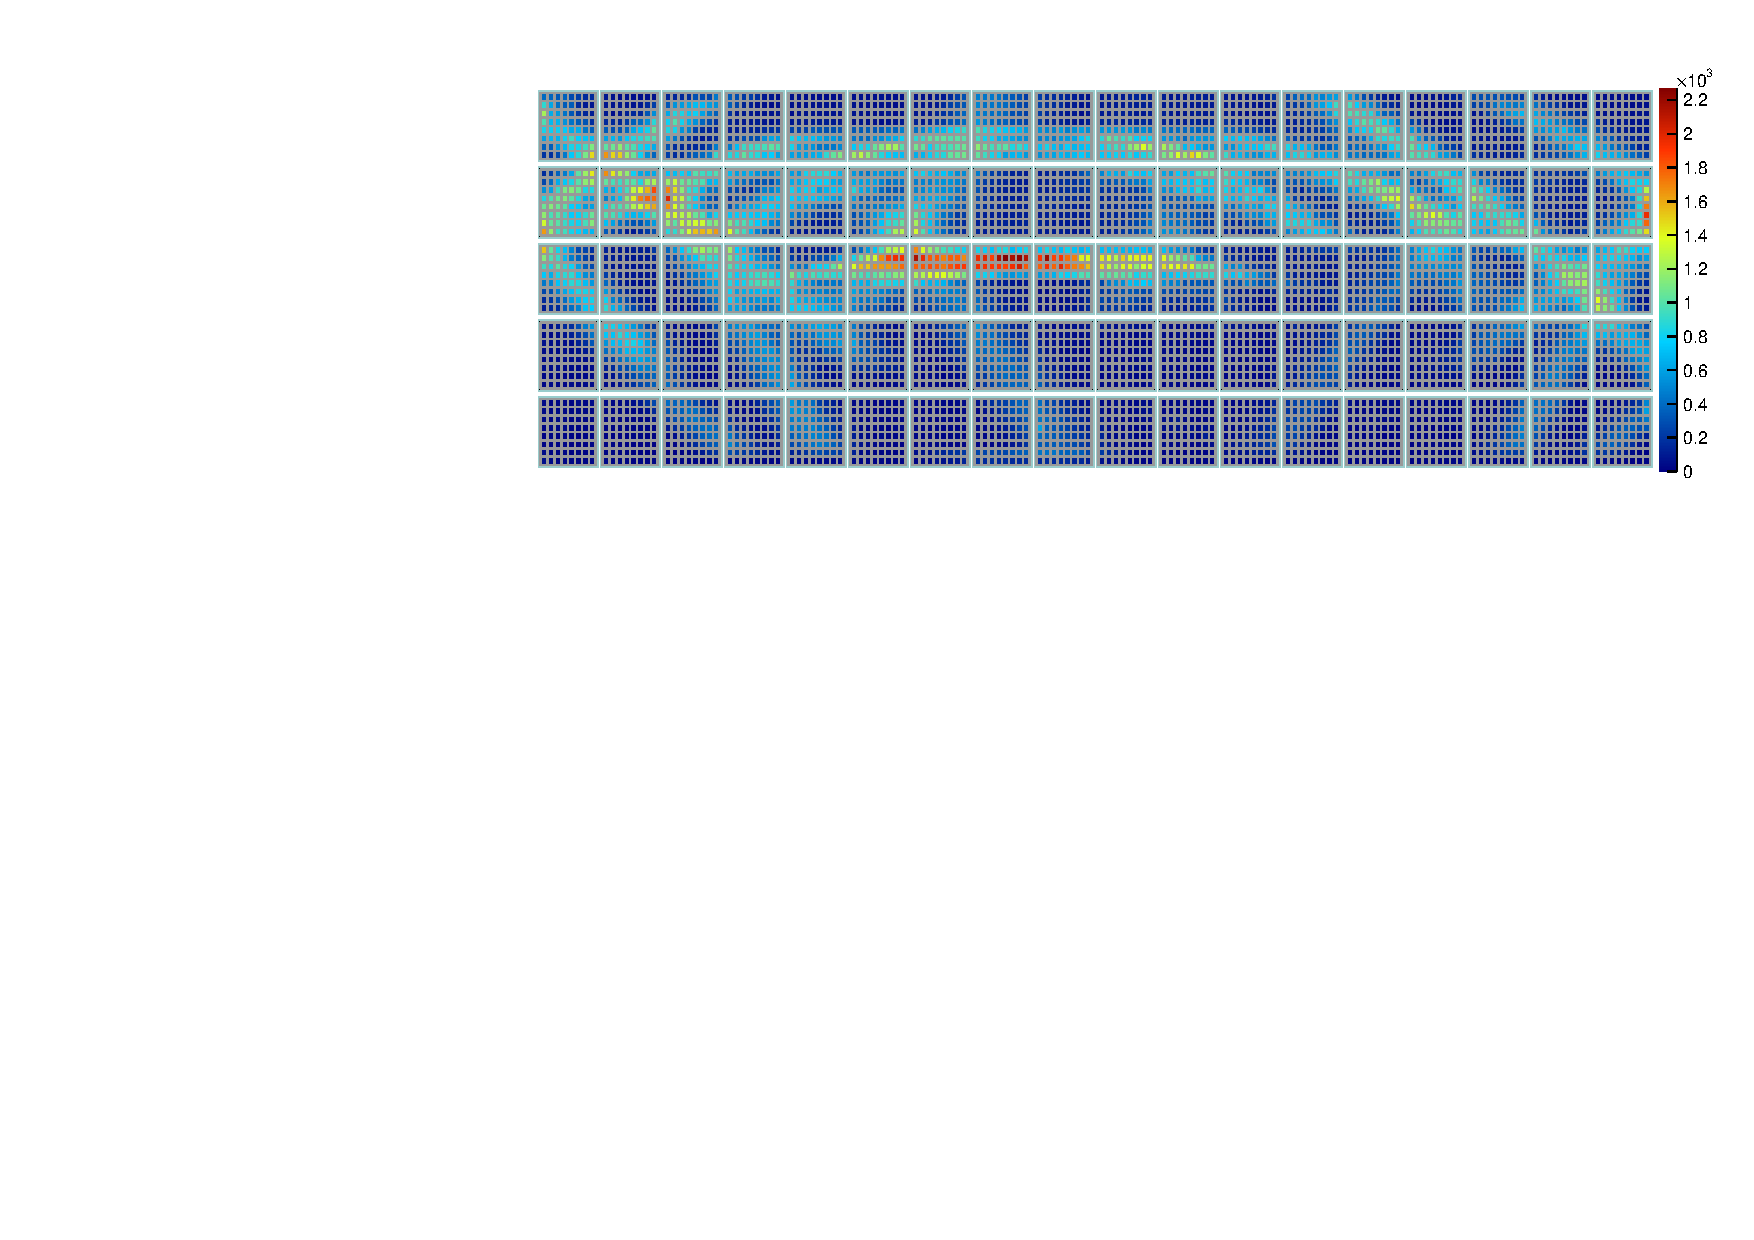
\includegraphics[angle=0,width=0.47\textwidth]{pics/kaons2GeV.pdf} \hspace{0.5cm} 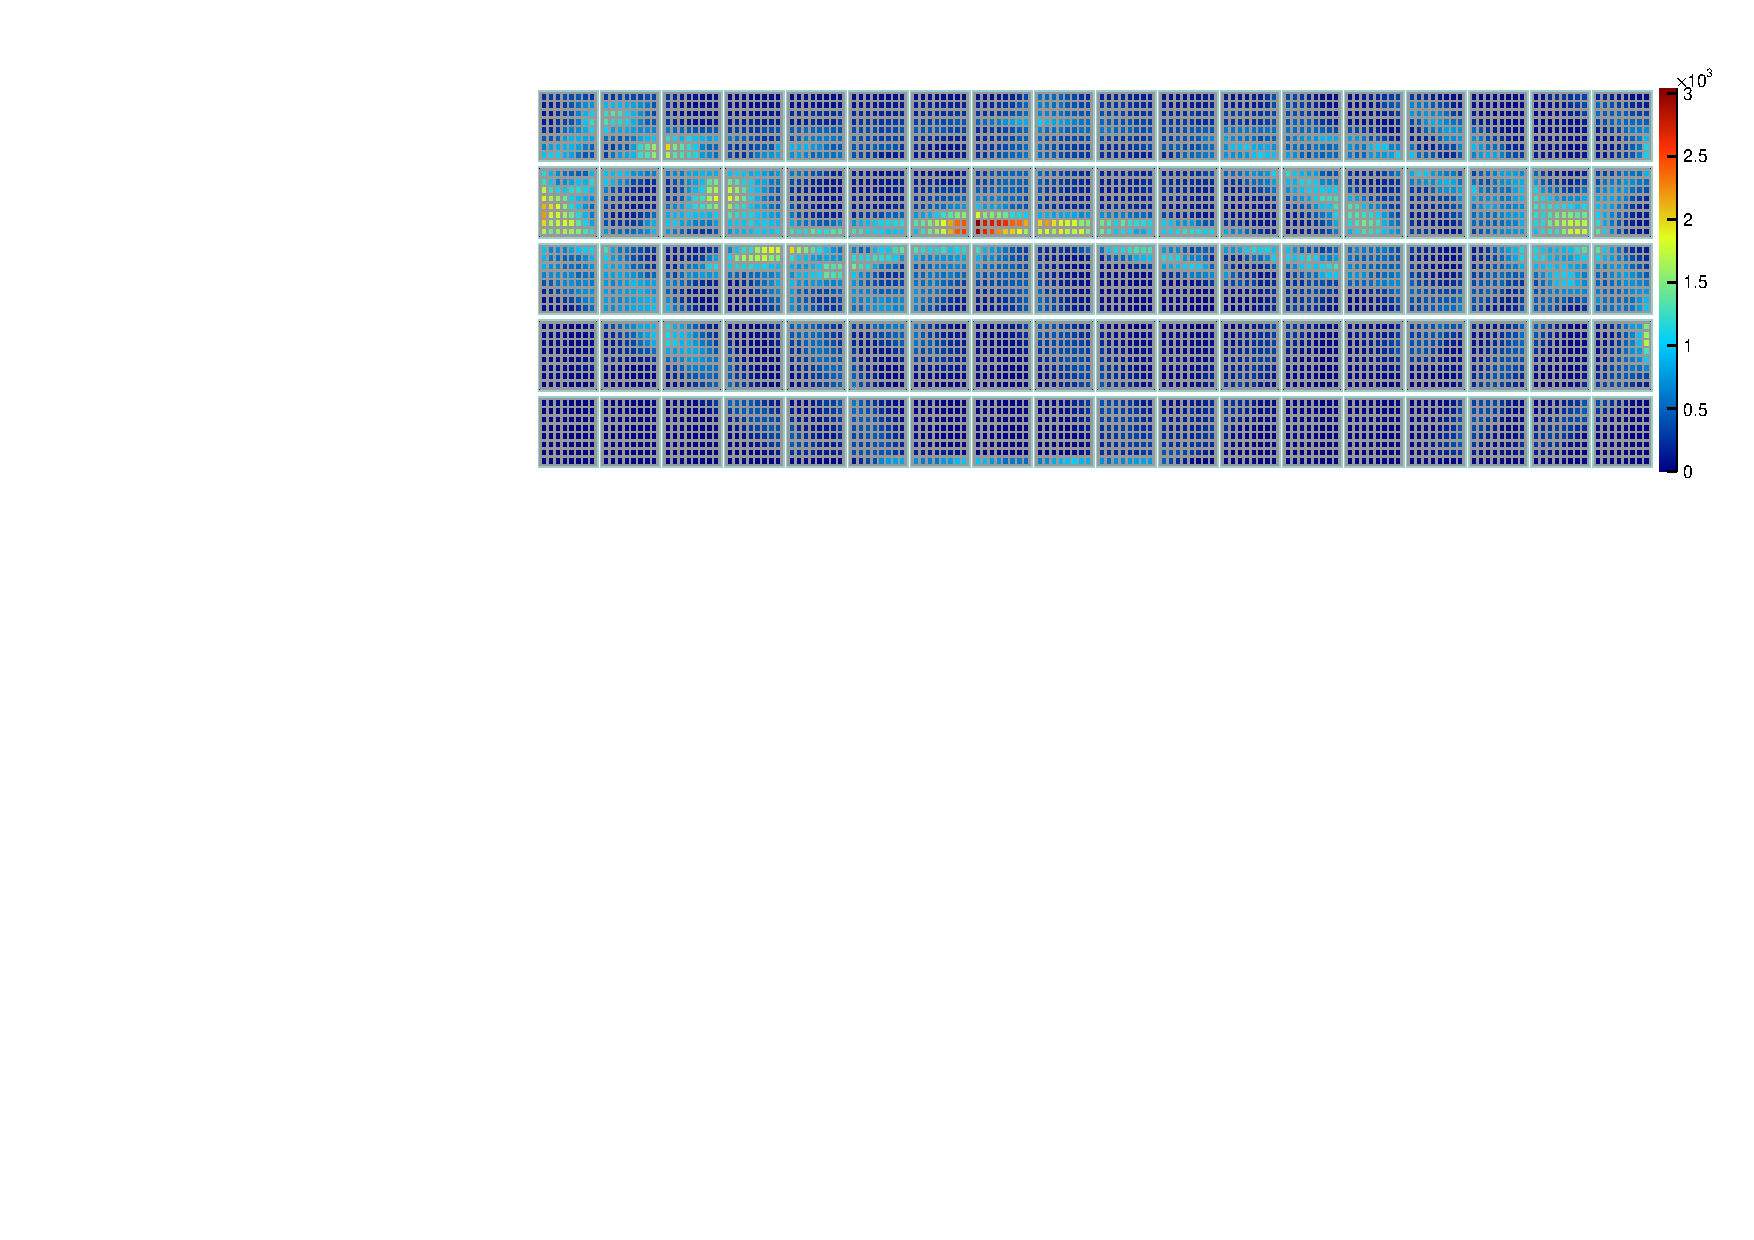
\includegraphics[angle=0,width=0.47\textwidth]{pics/pions2GeV.pdf}
\caption{\label{pic:hitpat1}
Typical \gluex DIRC hit patterns. The left column shows pions, and the right one -- kaons. 
Signals from single charged particles are shown in the upper row, and the cumulative patterns in the lower row.
One edge row of 18 PMTs is removed (should have been substituted with dummies. This idea then was transformed into distributing dummies according to the map shown in Fig.~\ref{pic:dummies}).
%Signals from single charged particles (upper row) look quite uncorrelated, and the cumulative patterns (bottom row) represent the complexity of the patterns. 
Samples of $40000$ single kaons and pions with momentum of 2 {\gev}/c and direction defined by $\theta = 1.2$\mydeg and $\phi = 90$\mydeg angles were used to create these plots.
}
\end{figure}

Typical \gluex DIRC hit patterns are shown in Fig.~\ref{pic:hitpat1}. DIRC does not try to reconstruct the shape of the hit pattern, but use different methods to compare hit patterns $(x,y,t)$\footnote{It is convenient to use a separate coordinate system on the photodetection plane. There $x$ axis goes along the long rows of PMTs containing $18$ sensors each, and $y$ axis goes along the short PMT rows of $6$ sensors each.} to expectations for different particle hypotheses ($e, \mu, \pi, K, p$).

%\begin{figure}[!h]
%\centering
%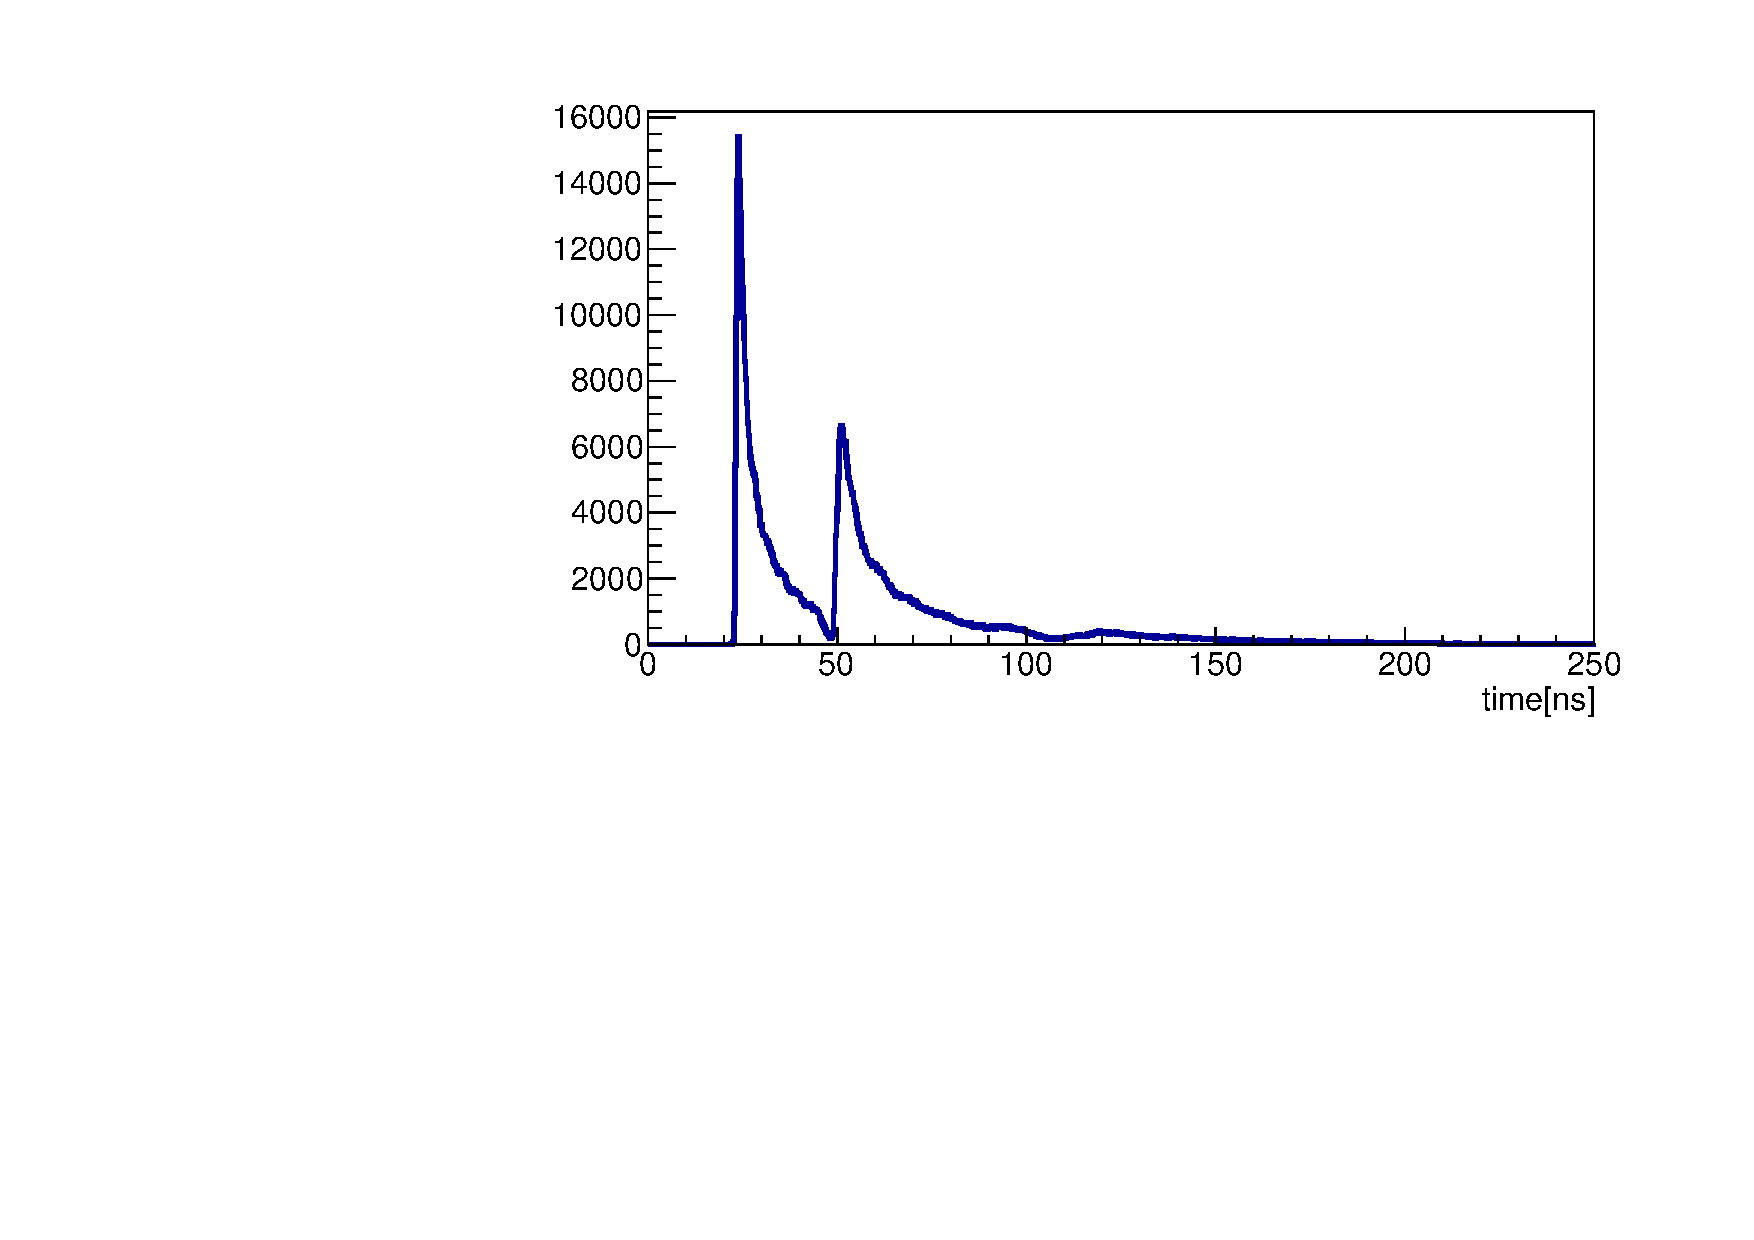
\includegraphics[angle=0,width=0.6\textwidth]{pics/Npho_th1_2_ph90.pdf}
%\caption{\label{pic:time}
%An example of the cumulative timing signal for charged kaons with momentum of 2 {\gev}/c and direction defined by $\theta = 1.2$\mydeg and $\phi = 90$\mydeg angles. The two peaks at $25$ ns and $55$ ns correspond to two groups of Cherenkov photons. The first group (left peak) contains direct photons, which were emitted towards the readout end of the bar unlike the second group (right peak), which first went to the mirror at the fuar end of the radiator, and then towards the optical box. The spread of the timing signal for one track is tens of nanoseconds. 
%The dip in the spectra around $48$ ns show photon loss due to the total internal reflection inside the radiator. 
%}
%\end{figure}

DIRC measures $(x,y,t)$ of each detected Cherenkov photon. In $(x,y)$ the cumulative hit patterns look like conic sections with additional reflections (see cumulative hit patterns for different charged particle configurations \url{http://web-docs.gsi.de/~rdzhigad/www/research/hit-pattern-vs-theta-phi}). In the coordinate space ($x ,y$) some parts overlap, but timing helps to separate them.
The exact way to use the timing information for the reconstruction will be discussed in the next sections.
%An example of the cumulative timing spectra for charged kaons with fixed momentum and direction is shown in Fig.~\ref{pic:time}. 

The number of detected photons is an important observable of the DIRC. A comparison between the measured and expected photon yield for different hypotheses at a given momentum help to separate between different particle types. Examples of the simulated number of detected photons for kaons and pions with different momenta are shown in Fig.~\ref{pic:npho}.

\begin{figure}[!h]
\centering
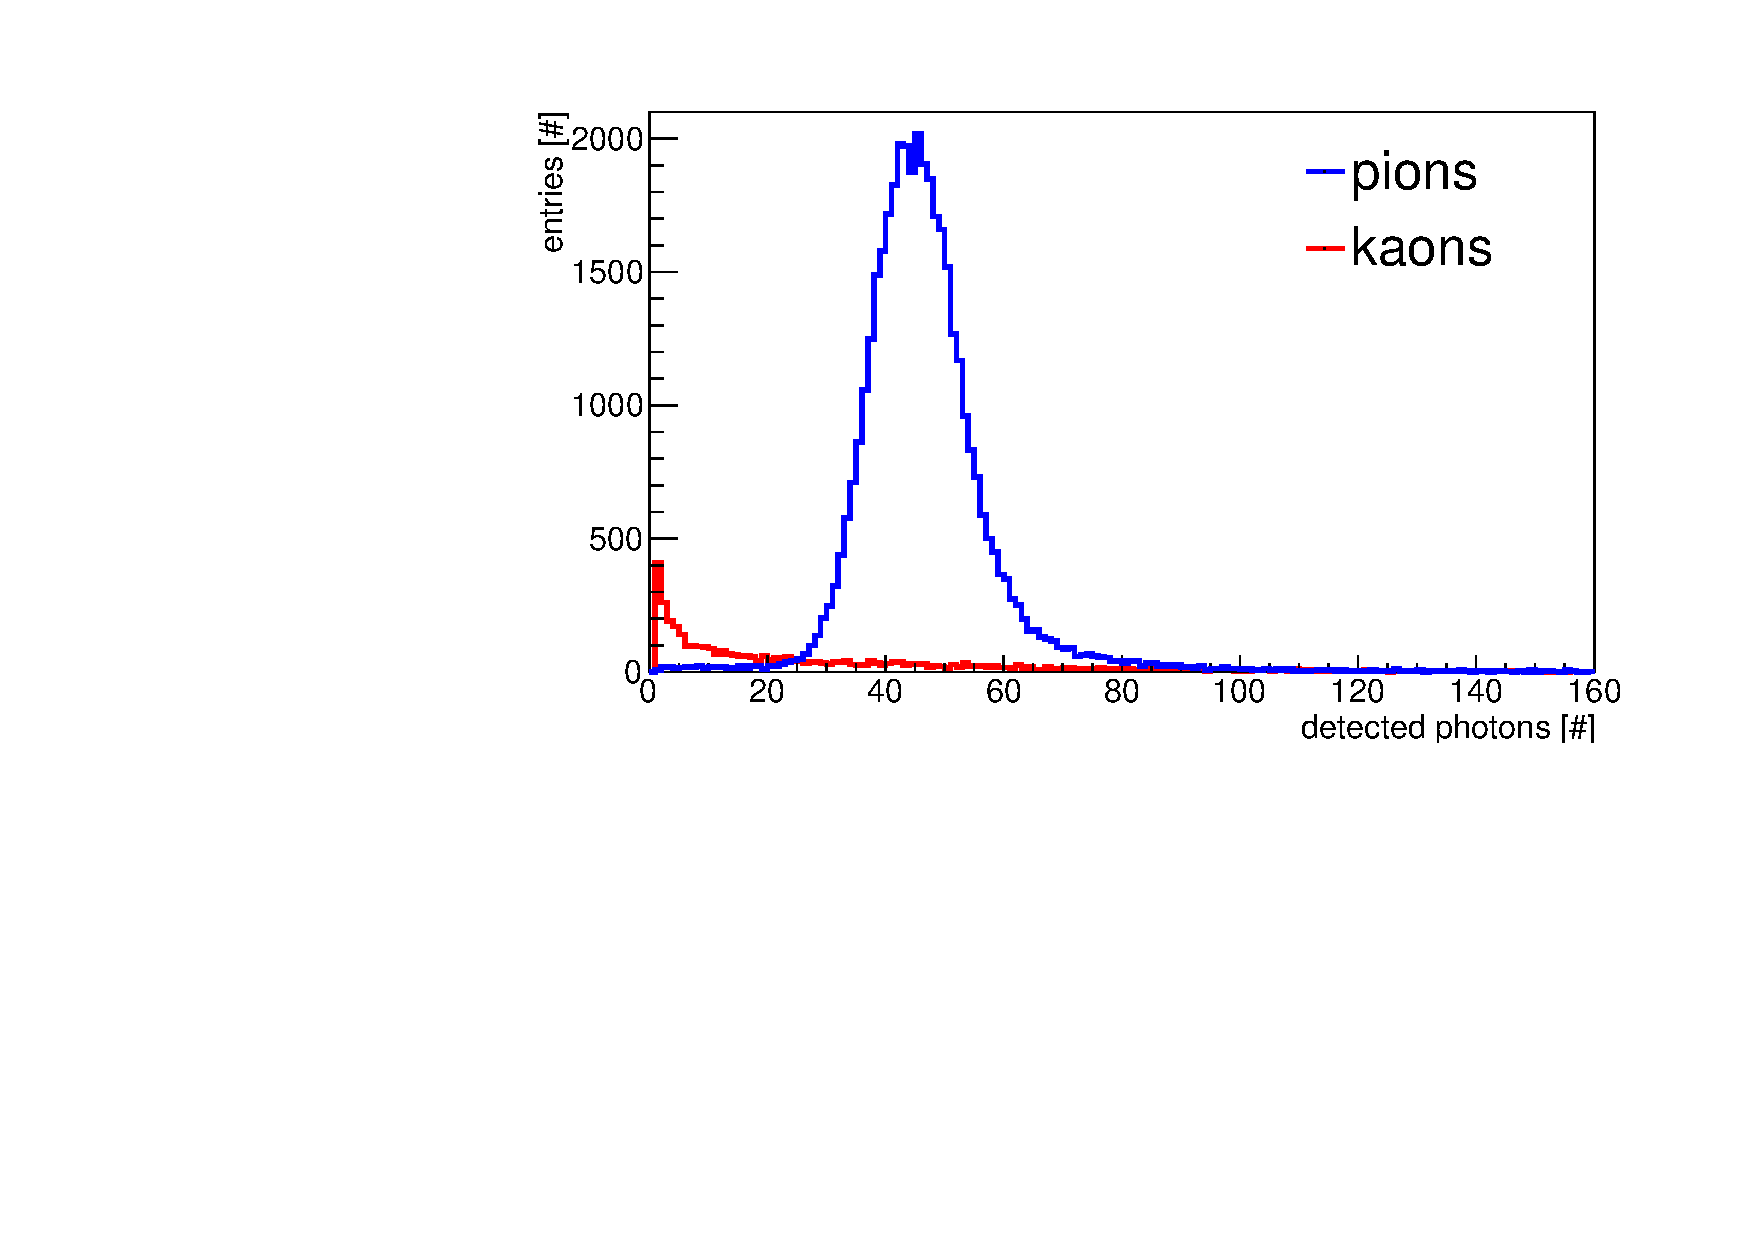
\includegraphics[width=0.43\textwidth]{pics/Npho0_5GeV.pdf} \put(-80.,50.){0.5 GeV/c} \hspace{0.5cm} 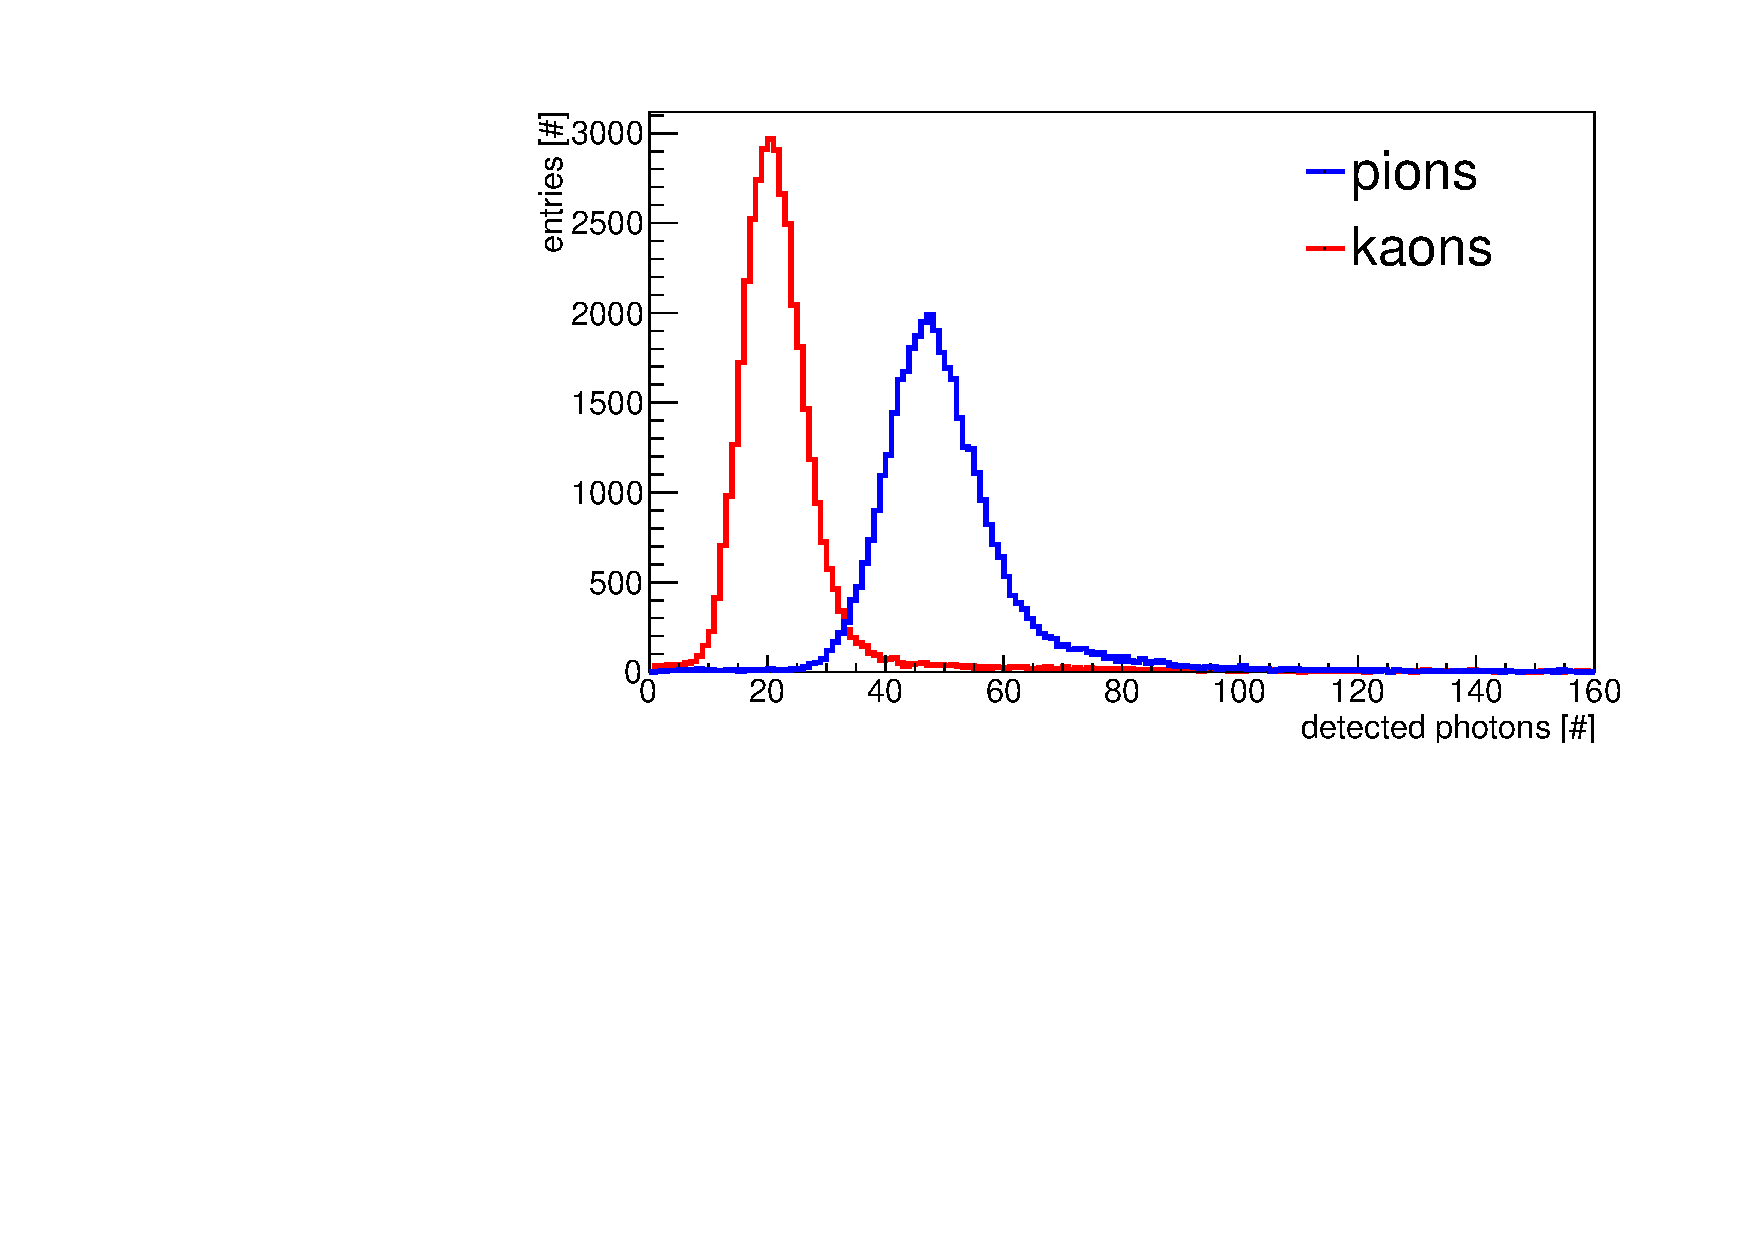
\includegraphics[width=0.43\textwidth]{pics/Npho0_8GeV.pdf} \put(-80.,50.){0.8 GeV/c}\\
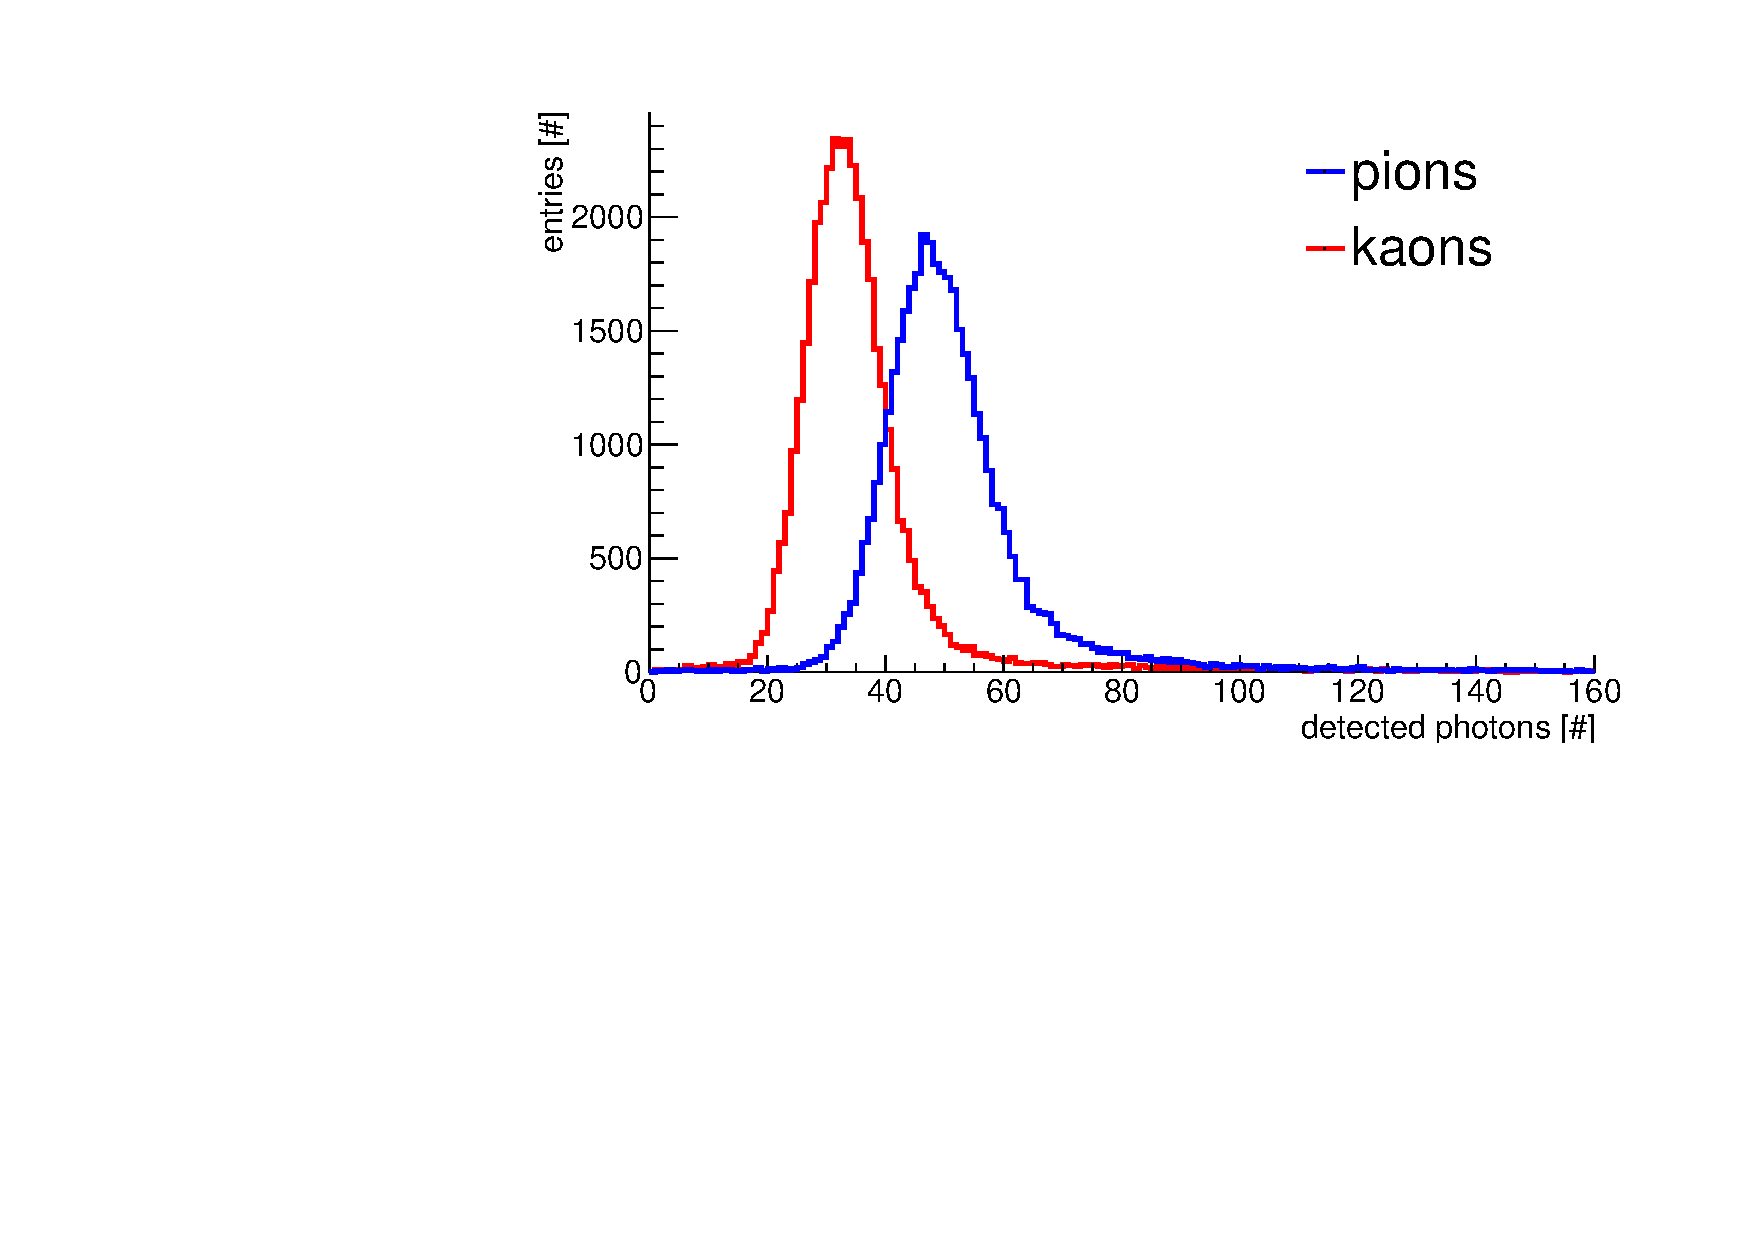
\includegraphics[width=0.43\textwidth]{pics/Npho1GeV.pdf} \put(-80.,50.){1 GeV/c} \hspace{0.5cm} 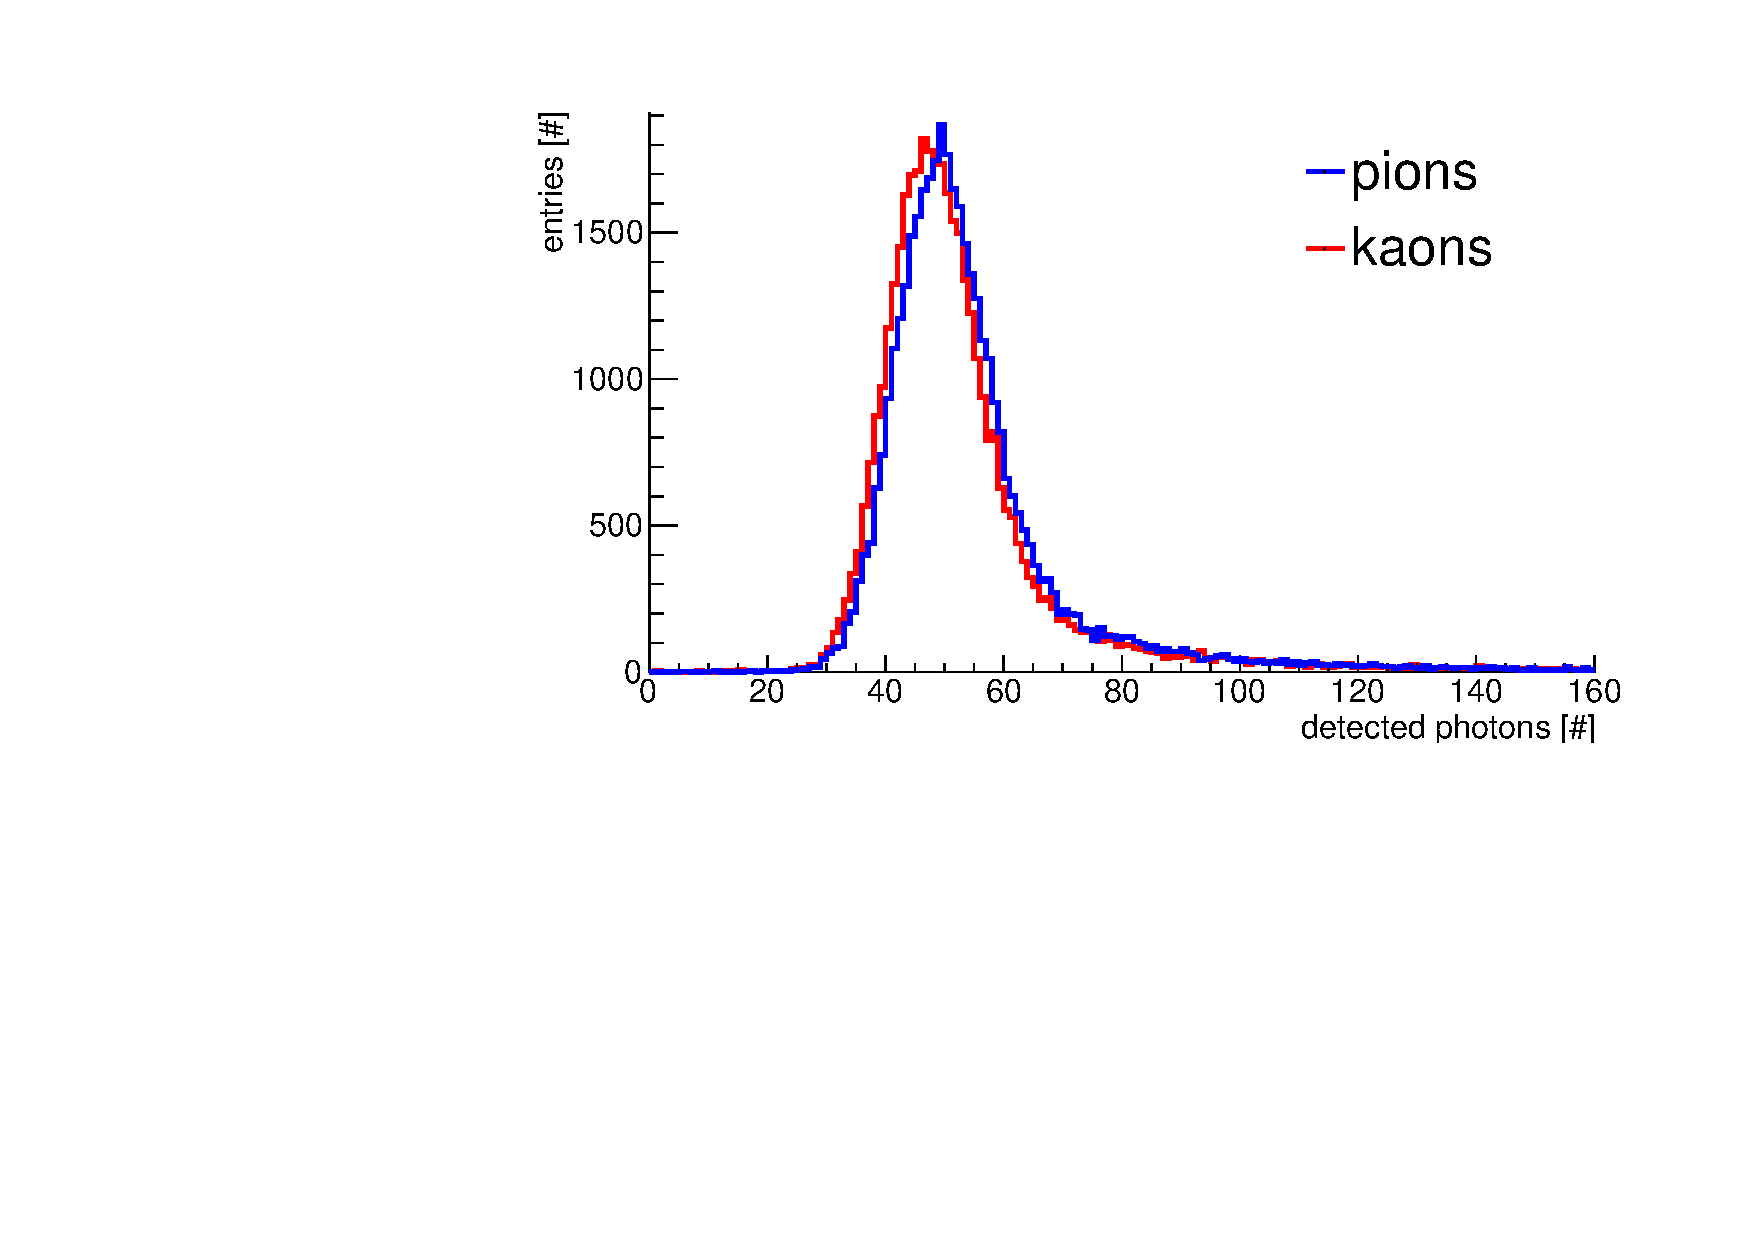
\includegraphics[width=0.43\textwidth]{pics/Npho3GeV.pdf} \put(-80.,50.){3 GeV/c}\\
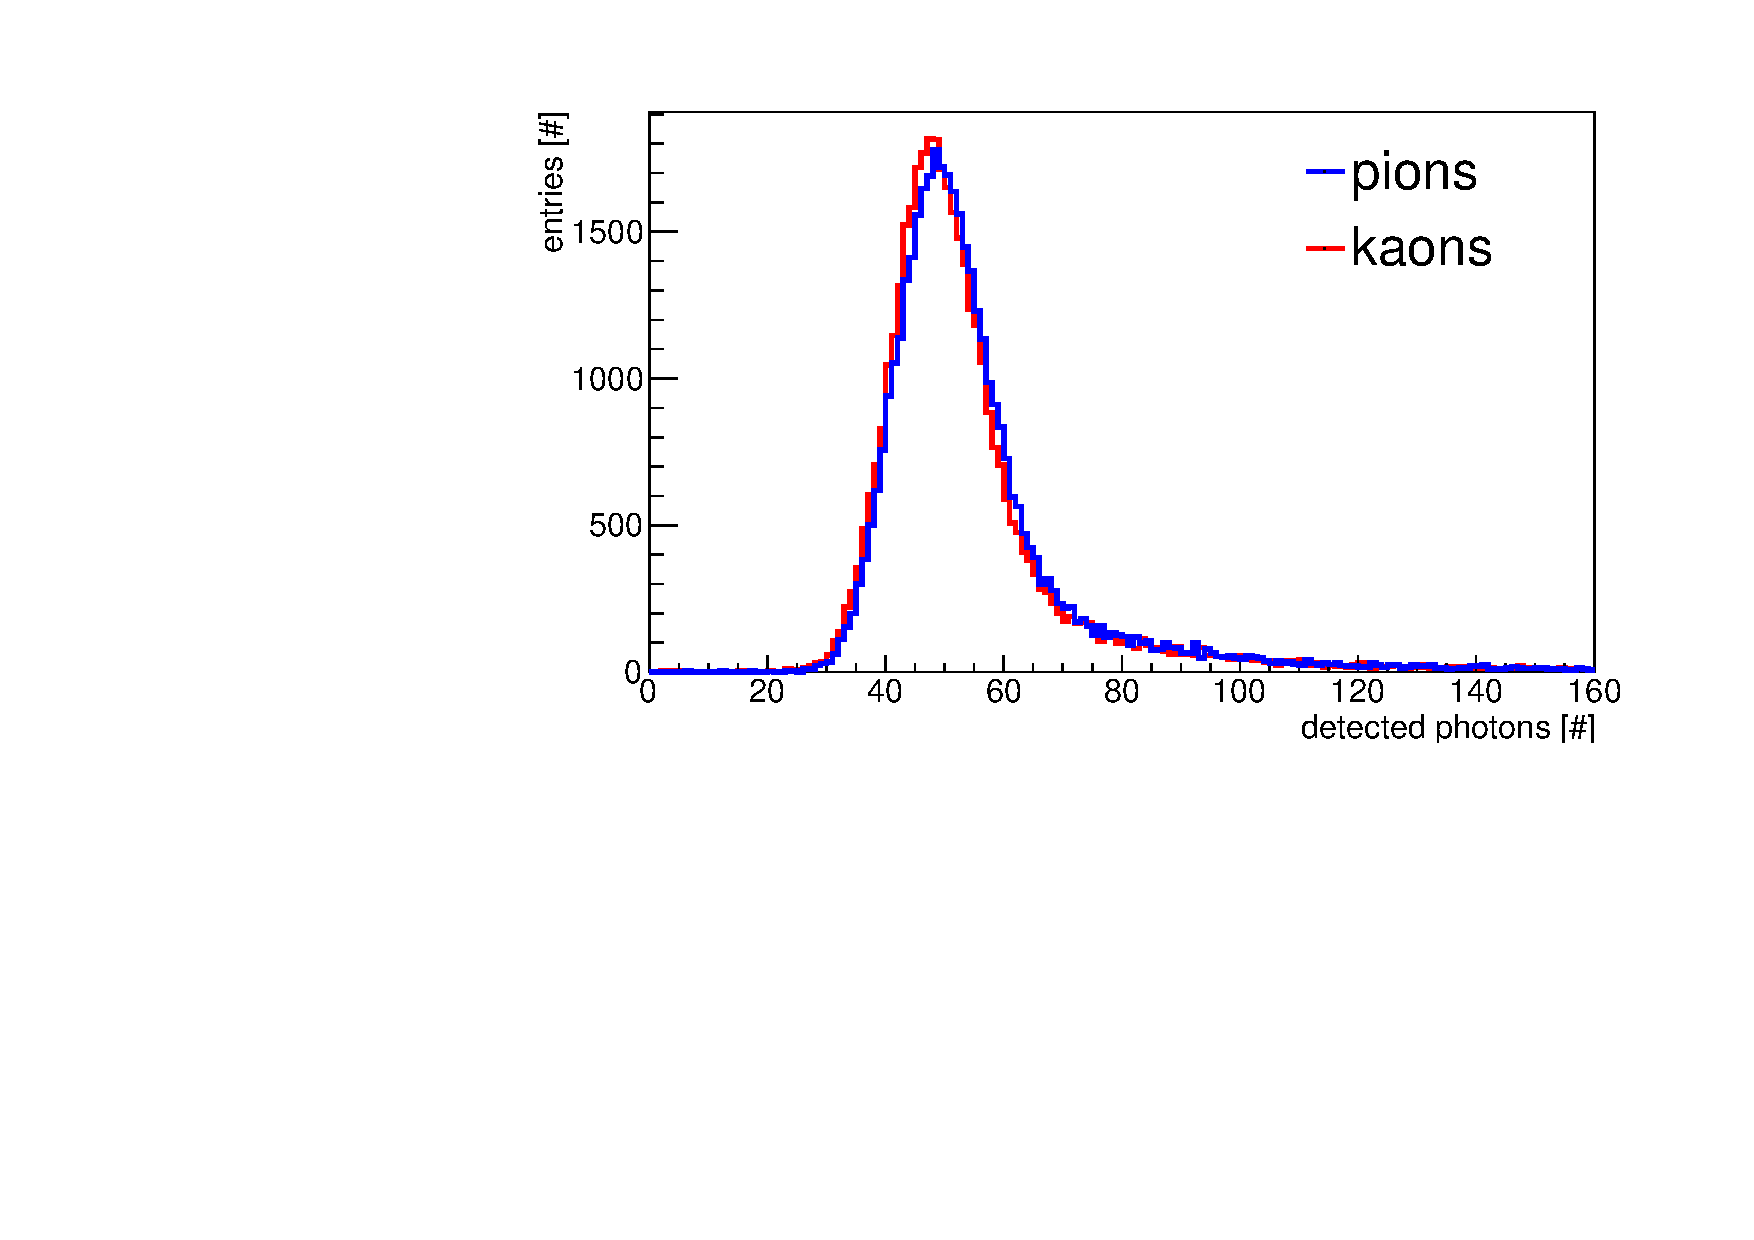
\includegraphics[width=0.43\textwidth]{pics/Npho4GeV.pdf} \put(-80.,50.){4 GeV/c} \hspace{0.5cm}
\caption{\label{pic:npho}
Simulated number of detected photons per track for kaons (red) and pions (blue) for particle direction defined by  $\theta = 4$\mydeg and $\phi = 90$\mydeg and different momenta.
}
\end{figure}

\begin{figure}[!h]
\centering
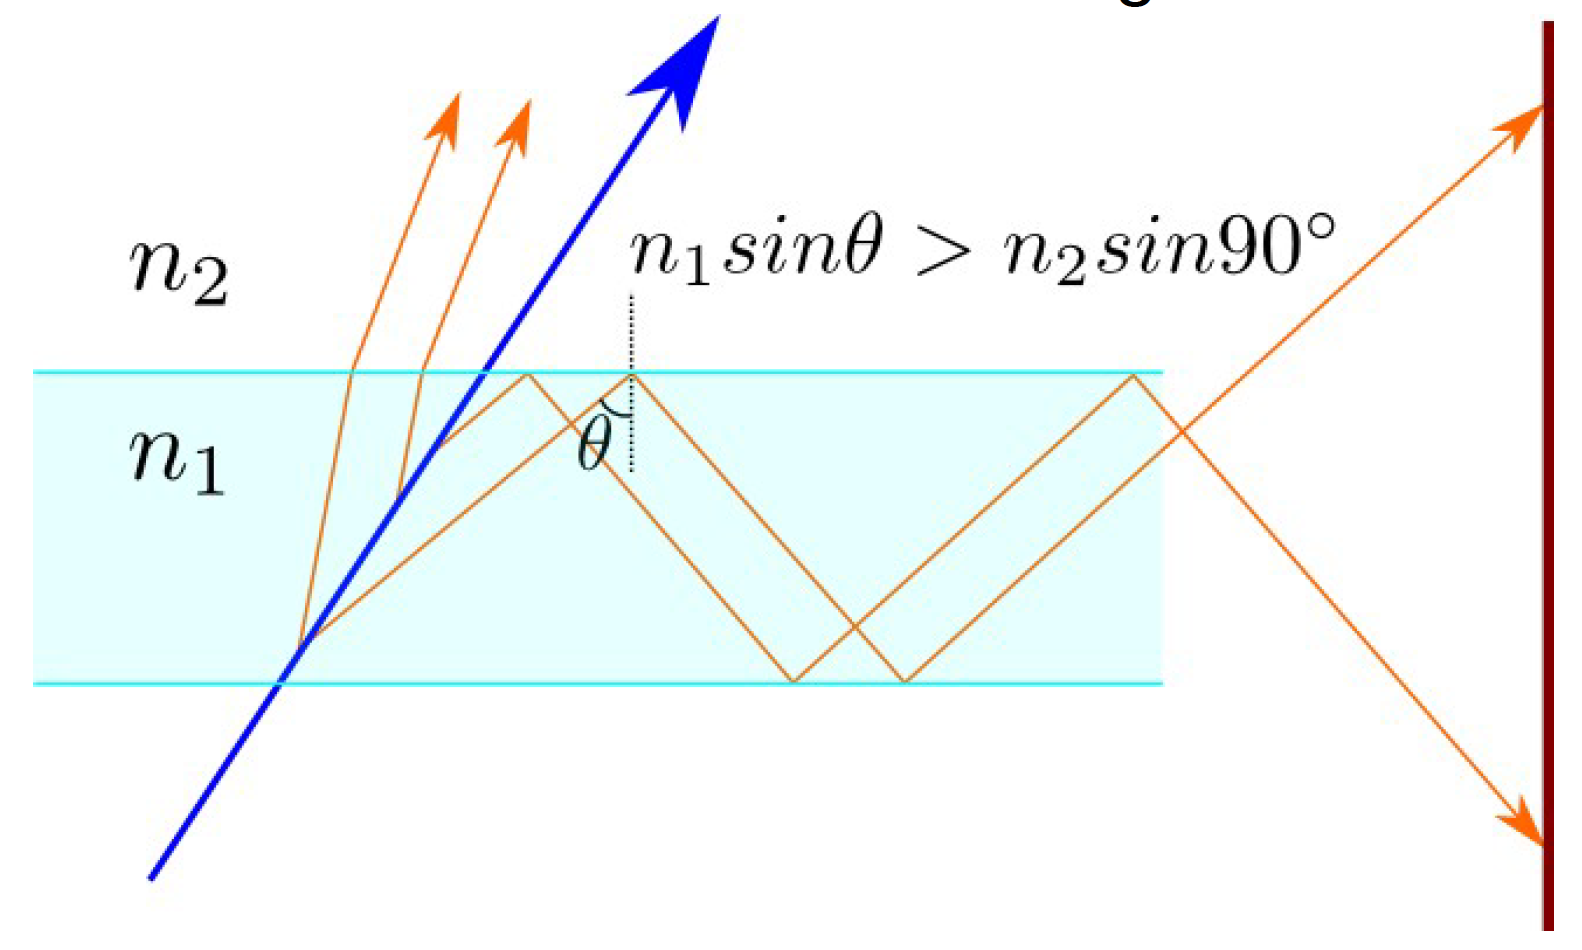
\includegraphics[width=0.5\textwidth]{pics/bas2.png}
\caption{\label{pic:bas2}
Illustration of the total internal reflection condition on the border between the fused silica ($n_{1}$) and air ($n_{2}$). Some Cherenkov photons do not satisfy the total internal reflection condition and escape the radiator. A fraction of the Cherenkov cone is internally reflected and thus can be transported to the photon detectors.
}
\end{figure}

DIRC has a specific timing signal with duration up to 100 ns. The formation of the signal is the following. When a charged particle crosses the radiator and produces Cherenkov photons on a cone, the total internal reflection condition defines which parts of the cone get trapped inside the radiator. Figure~\ref{pic:bas2} shows the case when the charged particle crosses the radiator at a rather shallow angle, so that only one side of the Cherenkov cone gets totally internally reflected. In case when the charged particle crosses the radiator almost perpendicularly, both sides of the Cherenkov cone satisfy the total internal reflection condition and, therefore, Cherenkov photons propagate towards both ends of the radiator. The ``direct'' photons propagate from the point of origin directly to the readout end of the bar (Fig.~\ref{pic:eta2300}, blue arrows), and ``reflected'' ones first go towards the bar end equipped with a mirror (Fig.~\ref{pic:eta2300}, red arrows). 

The DIRC timing signal might have one or two sharp time peaks, depending on the angle of the charged particle relative to the radiator sides. These time peaks correspond to direct and reflected photons. Examples of timing spectra for different radiators and several x positions of the charged particle along the DIRC radiator are shown in Fig.~\ref{pic:timedist}. Direct and reflected photons are shown in blue and red respectively.

\begin{figure}[!h]
\centering
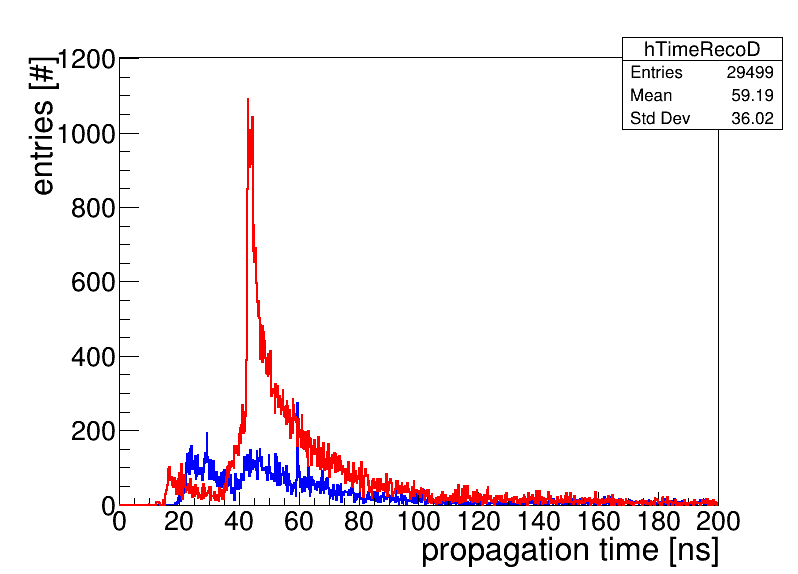
\includegraphics[width=0.45\textwidth]{pics/bar0_xm65.png} \put(-80.,90.){bar 0} \put(-80.,60.){x = -65 cm} \hspace{0.5cm} 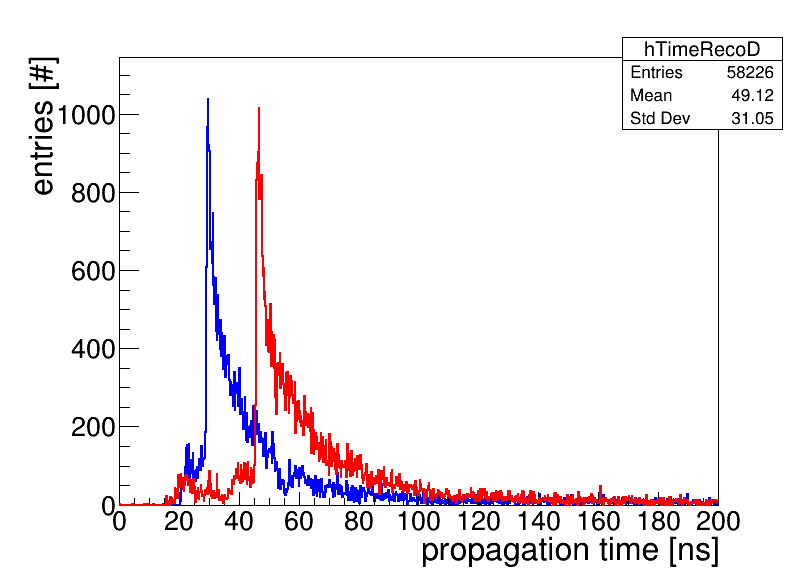
\includegraphics[width=0.45\textwidth]{pics/bar0_xm40.png} \put(-80.,90.){bar 0} \put(-80.,60.){x = -40 cm}\\
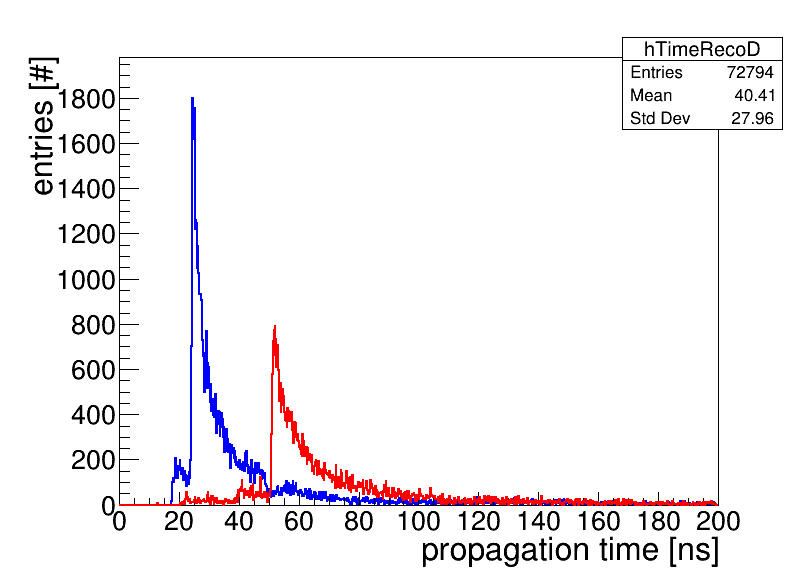
\includegraphics[width=0.45\textwidth]{pics/bar0_x0.png} \put(-80.,90.){bar 0} \put(-80.,60.){x = 0} \hspace{0.5cm} 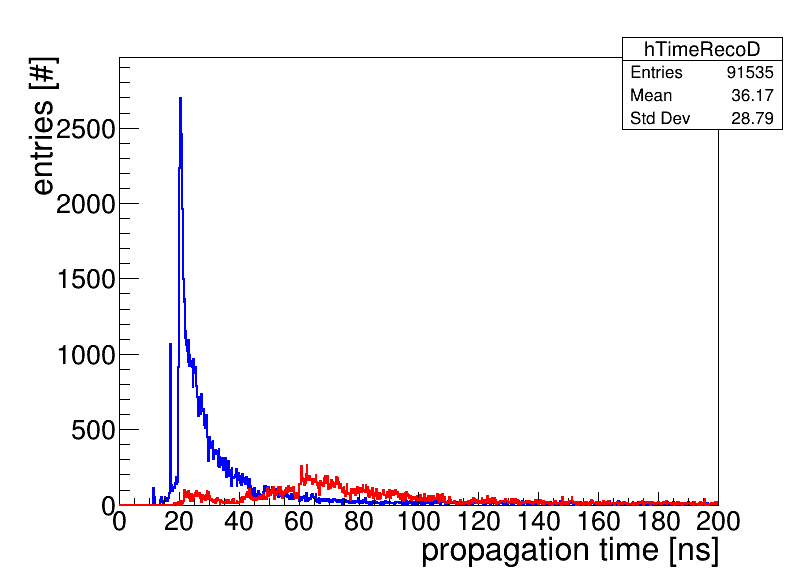
\includegraphics[width=0.45\textwidth]{pics/bar0_x45.png} \put(-80.,90.){bar 0} \put(-80.,60.){x = 45 cm}\\
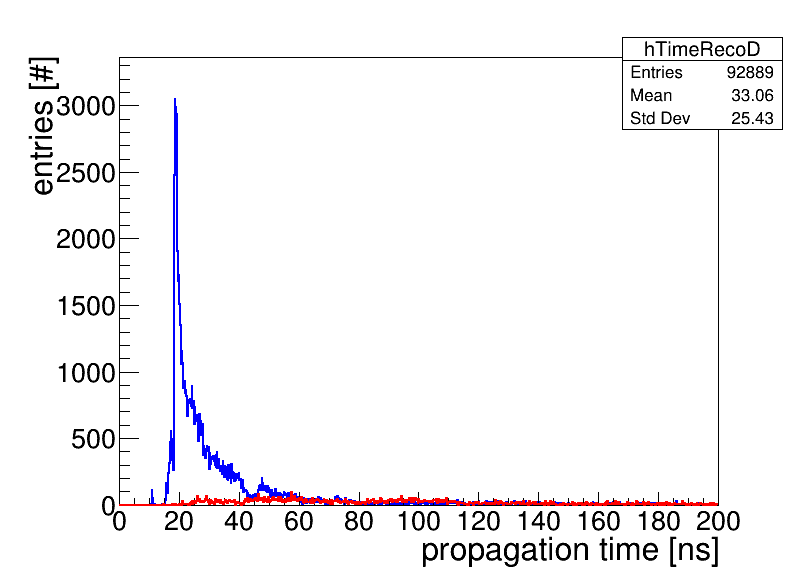
\includegraphics[width=0.45\textwidth]{pics/bar0_x65.png} \put(-80.,90.){bar 0} \put(-80.,60.){x = 65 cm} \hspace{0.5cm} 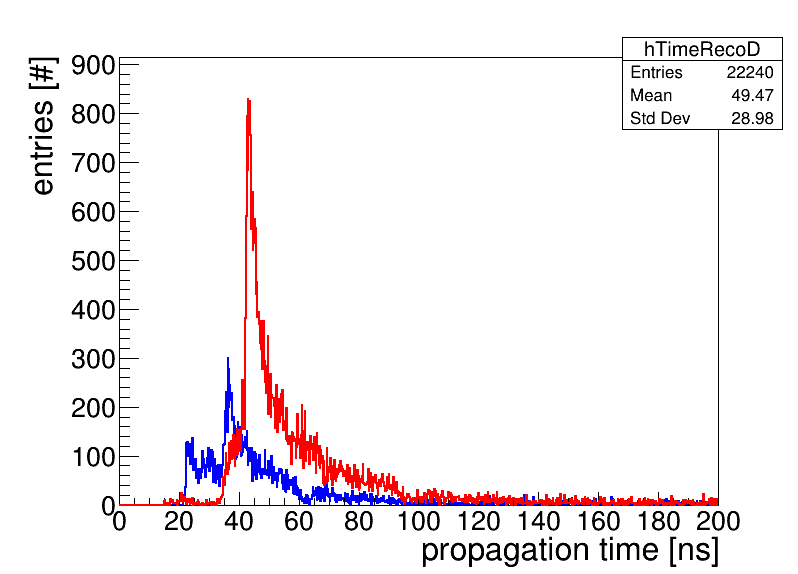
\includegraphics[width=0.45\textwidth]{pics/bar11_xm65.png} \put(-80.,90.){bar 11} \put(-80.,60.){x = -65 cm}
\caption{\label{pic:timedist}
Timing spectra for 500 single track events of kaons with momentum of 4 GeV/$c$ originating from the interaction point (0, 0, 65) cm and hitting radiators 0 and 11 at a given x position. The blue spectrum corresponds to the direct photons (see text for details), and the red spectrum -- for reflected photons. Irregular peaks like for bar 0, x = 45 cm at 17 ns correspond to signals from secondary particles.
}
\end{figure}

\input{led.tex}

\section{Reconstruction}

Three reconstruction approaches are being implemented into the GlueX Software. The geometrical reconstruction is fully implemented and can be used at the beginning of the DIRC operation. The time-based imaging  needs some development effort. The KDE-based reconstruction was very useful for the design work. This method is to be implemented into the software.

\subsection{Geometrical Reconstruction}
\label{sec:gr}

The geometrical reconstruction is based on the \babar DIRC approach~\cite{bdirc1}. This approach transforms the knows spacial positions of the bar through which the track passed and the pixel with a detected photon into the Cherenkov coordinate system. The direction of a detected photon is approximated by the three-dimensional vector between the center of the bar face, where the small wedge is attached, and the center of the pixel, taking refraction and reflection at all material interfaces into account. Those photon direction vectors are combined with the particle momentum vector, provided by the tracking system, to determine the Cherenkov angle $\theta_{C}$ for each photon (see Fig.~\ref{pic:lut1}). 

The full simulation is used to calculate the photon direction vectors for every possible bar-pixel combination. This is done by simulating the production of optical photons at the end of the bar and tracking them through the small wedge and optical box to the sensor pixels. Photons are produced with polar angles between $90$\mydeg and $270$\mydeg and azimuthal angles between $0$\mydeg and $360$\mydeg.
%, and for every pixel the average direction vector at the production point is stored in a look-up table (LUT).
One entry of the look-up table (LUT), corresponging to a single pixel, might contain more than one initial photon direction. E.g. in Fig.~\ref{pic:lut2} two photons with initial momenta $\vec k_1$ and $\vec k_2$ follow different trajectories inside the photon camera ending up in the same pixel. 
Groups of photons following each trajectory (e.g. blue and purple in Fig.~\ref{pic:lut2}) are collected separately, for each of the group the initial photon directions are averaged, and the mean values of the direction components are stored in the LUT. For a particular radiator bar, one entry of the look-up table consist of a pixel number, a set of photon direction vectors and their propagation times inside the small wedge and the photon camera. To produce a complete look-up table for the whole optical box, 48 simulations with a particle gun located at the end of each radiator are needed. A simulation with about 10 million optical photons per radiator results into a LUT with sufficient statistics.

\begin{figure}[!h]
\centering
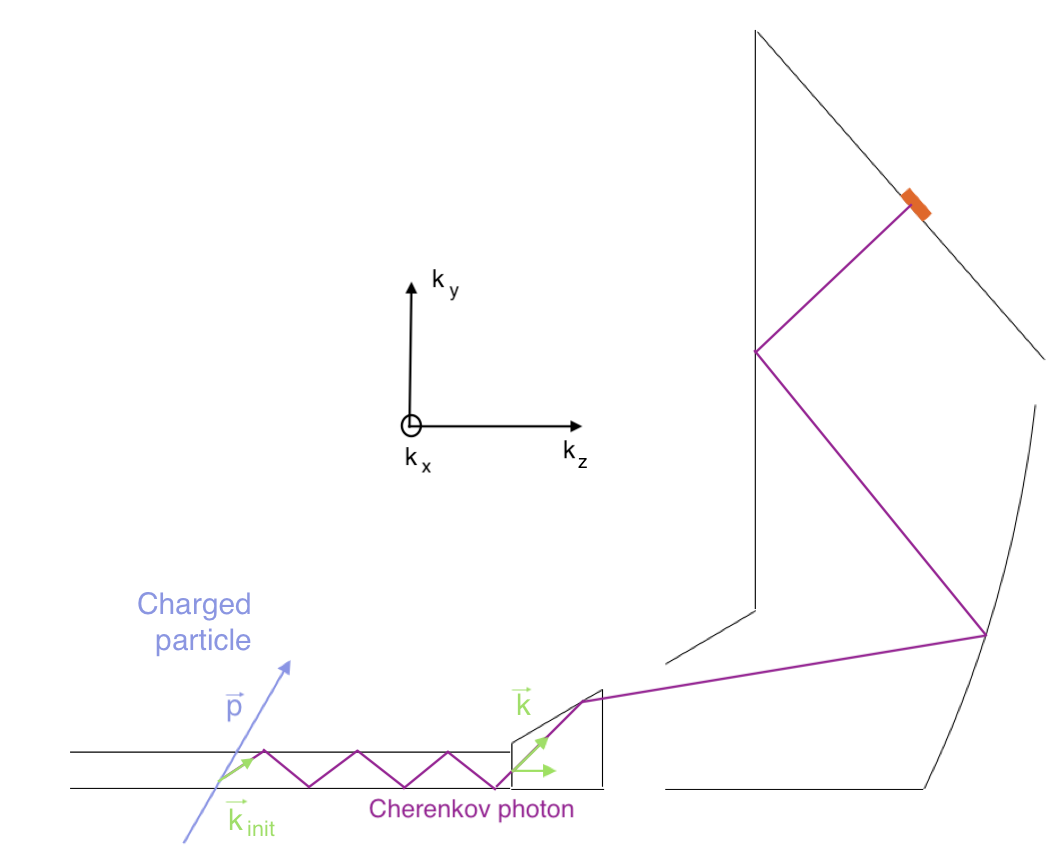
\includegraphics[clip, trim=0.5cm 0.0cm 0cm 0.cm,width=0.6\textwidth]{pics/lut3.png}
\caption{\label{pic:lut1}
The concept of the geometrical reconstruction. One example Cherenkov photon is emitted by the charged particle. The photon direction $\vec k$ is an estimator of the initial photon direction $\vec k_{init}$ and is used to reconstruct $\theta_{C}$ for this photon (using charged particle direction $\vec p$). 
%The photon transportation is described in the bar coordinate system, shown in the insert, which differs from the \gluex coordinate system used so far. In that case a reflection off a particular side results into a sign flip of the corresponding photon direction component.
}
\end{figure}

\begin{figure}[!h]
\centering
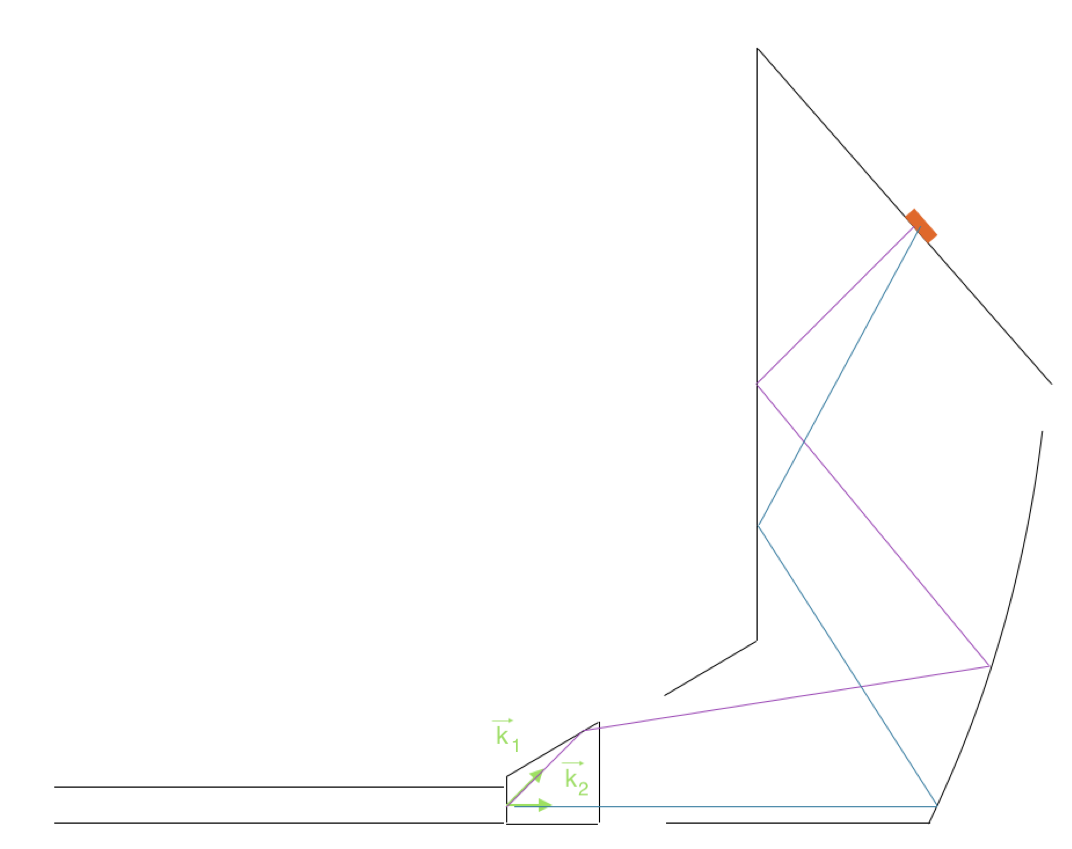
\includegraphics[clip, trim=0.5cm 0.cm 0cm 0.cm,width=0.6\textwidth]{pics/lut1.png}
\caption{\label{pic:lut2}
An illustration of one entry of the look-up table. Two photons with direction vectors $\vec k_{1}$ and $\vec k_{2}$ originate at the center of the bar, propagate throught the optical box, and end up in the same pixel. The look-up table entry corresponding to the shown pixel contains all possible propagation paths, including $\vec k_{1}$ and $\vec k_{2}$, and the associated propagation times in the small wedge and photon camera.
}
\end{figure}

The reconstruction procedure is the following: each particle crossing the DIRC wall yields a set of hit pixels (e.g. see upper row in Fig.~\ref{pic:hitpat1}). Each detected photon has a set of $N_{amb}$ solutions for the $\vec k$ vectors stored in the LUT. The true photon direction is then $N_{amb}$ ways ambiguous. Additional reconstruction ambiguities arise from the fact, that the exact photon path during the many internal reflections inside the bar is unknown.  
Each photon direction ambiguity inside the bar corresponds to a reflection off a radiator side. In the bar coordinate system shown in the insert of Fig.~\ref{pic:lut1} a photon reflection off a particular radiator side leads to the sign flip for the corresponding photon direction component. Eight different photon directions are possible inside the bar (sign flips for forward/backward, top/bottom, and left/right directions). They are taken into account by combining the direction from the LUT in eight different ways with the particle direction, leading to up to eight values for the recontructed photon Cherenkov angle for each $\vec k$ from the LUT entry.
Taking into account both types of ambiguities: $N_{amb}$ inside the photon camera and $8$ inside the radiator bar, for some angles a total number of $50$ and more photon directions is considered in the reconstruction.  This number is reduced by taking into account only photon directions that are internally reflected inside the bar and by requiring the photon Cherenkov angle to be smaller than 1000 mrad ($\approx 57$\mydeg).

%The reconstruction procedure is the following. Each event (a charged particle of some particle type and momentum crosses the DIRC wall) yields a set of hit pixels (e.g. see Fig.~\ref{pic:hitpat1}). Each detected photon has a set of solutions for the $\vec k$ vectors stored in the ''look-up'' table (see Fig.~\ref{pic:lut2}). 
%A three-dimensional photon direction vector $\vec k$ (see Fig.~\ref{pic:lut1}) origins from the center of the bar end and defines the photon path through the optical box ending in the given pixel.  
%Each $\vec k$ vector yields a set of $8$ solutions for the initial photon direction $\vec k_{init}$ (see Fig.~\ref{pic:lut1}), as the photon can effectively be reflected off any side inside the bar (see bar coordinate system depicted in Fig.~\ref{pic:lut1}).
%Together with the track direction, each $\vec k_{init}$ gives one hypothesis for the reconstructed Cherenkov angle of the photon. 

\begin{figure}[!h]
\centering
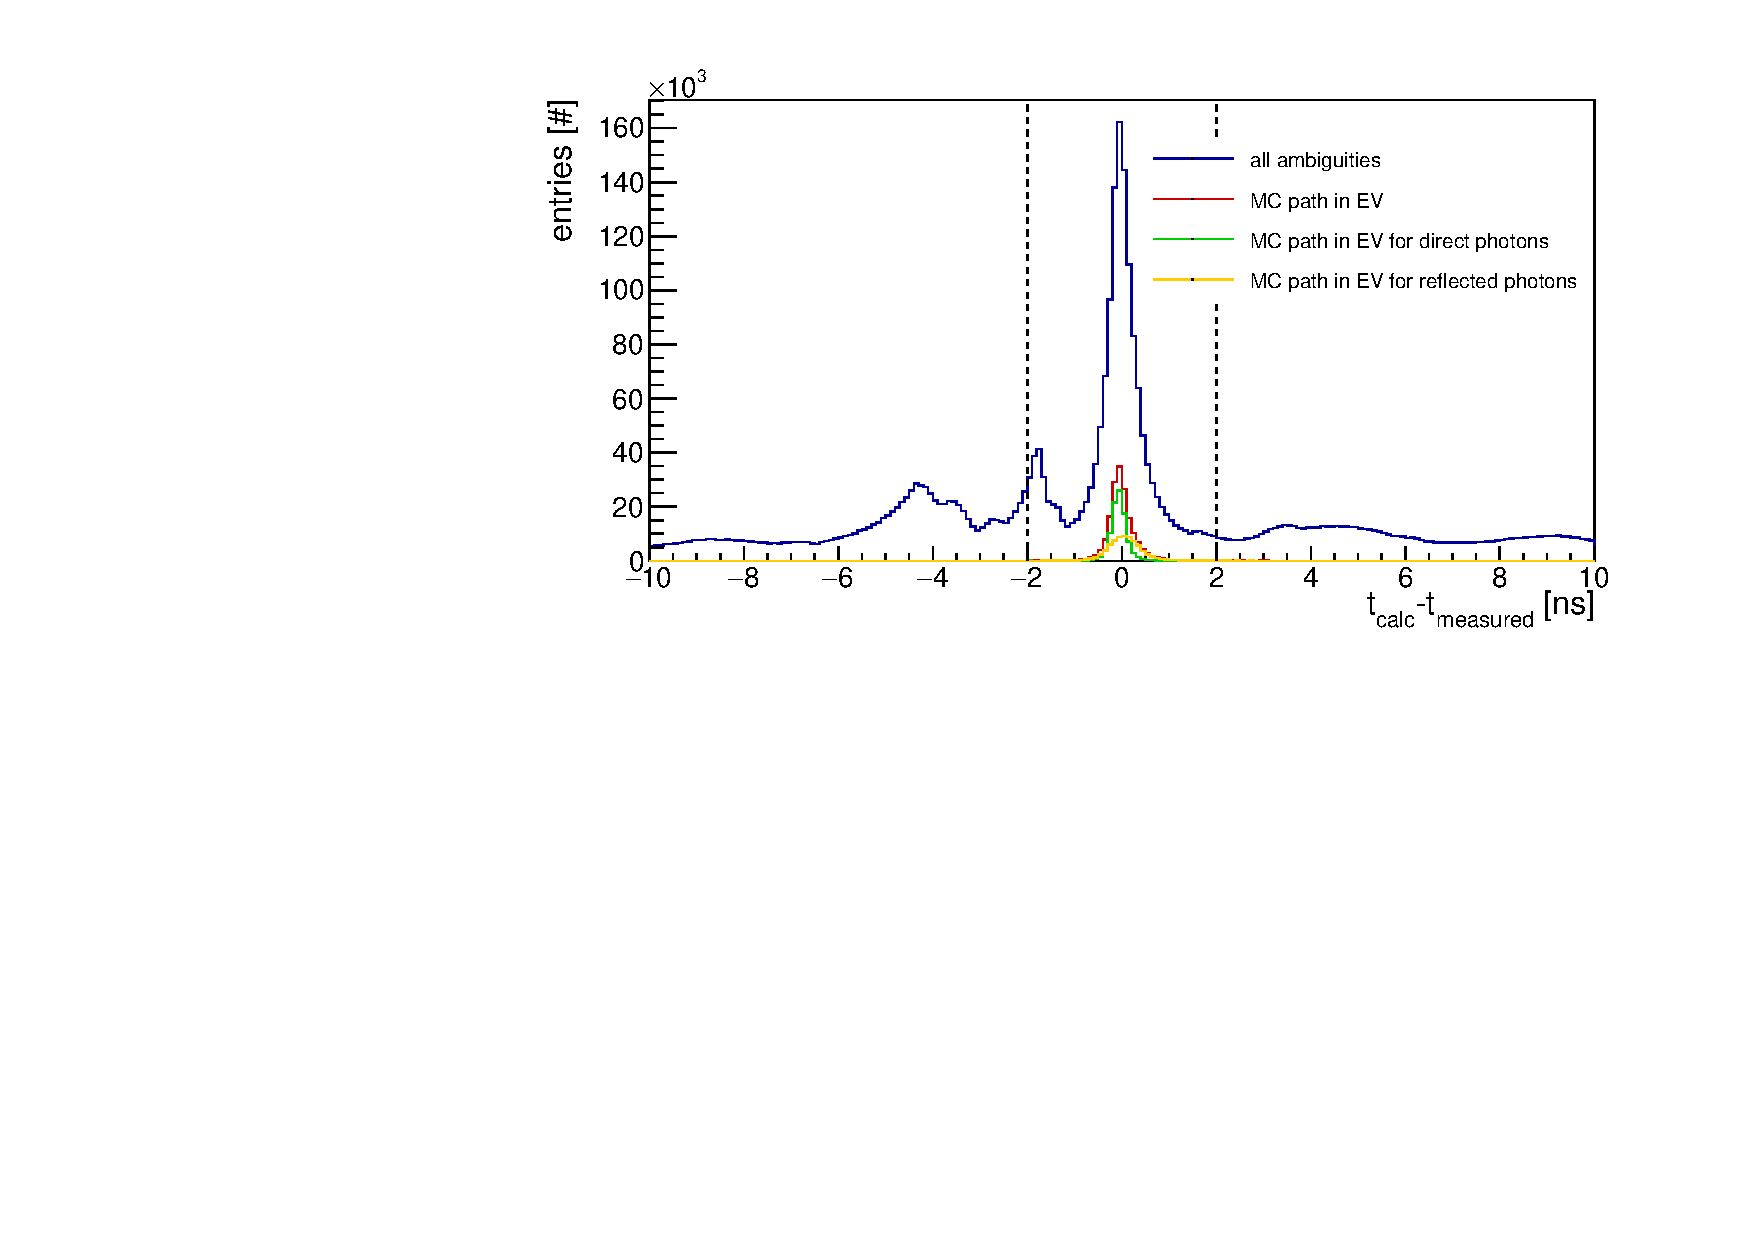
\includegraphics[width=0.8\textwidth]{pics/hDiff.pdf}
\caption{\label{pic:dtime}
Difference between measured and expected arrival time of Cherenkov photons. The blue line shows all solutions including bar and photon camera ambiguities. The red line includes bar ambiguities and a truth photon path inside the photon camera. The green and yellow lines show contributions to the red distribution by direct photons and reflected on the mirror at the radiator end photons respectively. The path length for direct photons is several times shorter than for the reflected photons, therefore the time difference gets less smeared for the green, than for the yellow distribution. The dashed lines show the applied cut for $|\Delta t| < 2$ ns. The plot is for 1000 pions with momentum of 4 \gev/c and direction defined by $\theta = 1$\mydeg and $\phi = 90$\mydeg angles.
}
\end{figure}

Most of the reconstructed photon paths correspond to Cherenkov angles far away from the expected value and form a combinatorial background under the peak associated with the correct photon path. A further reduction of the combinatorial background is achieved by selecting the difference between the measured and expected arrival time of the photon less than 2 ns (see Fig.~\ref{pic:dtime}). The expected arrival time is calculated as a sum of the photon propagation times inside the bar and photon camera. The latter is taken from the LUT. The photon propagation time inside the radiator is calculated based on the photon path, reconstructed using photon direction from the LUT, and the group velocity for photons with average wavelength of $376$ nm (see the energy spectrum of detected photons in Fig.~\ref{pic:lam}).

\begin{figure}[!h]
\centering
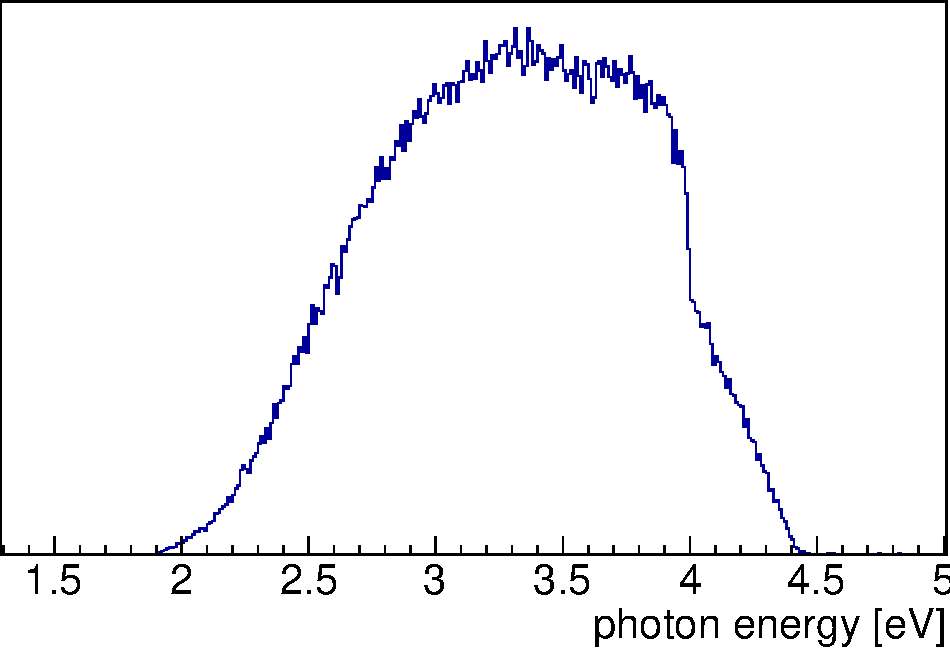
\includegraphics[width=0.5\textwidth]{pics/lam.pdf}
\caption{\label{pic:lam}
Simulated energy spectrum for detected Cherenkov photons. The mean value is $3.3$ eV, which corresponds to $376$ nm.
}
\end{figure}

\begin{figure}[!h]
\centering
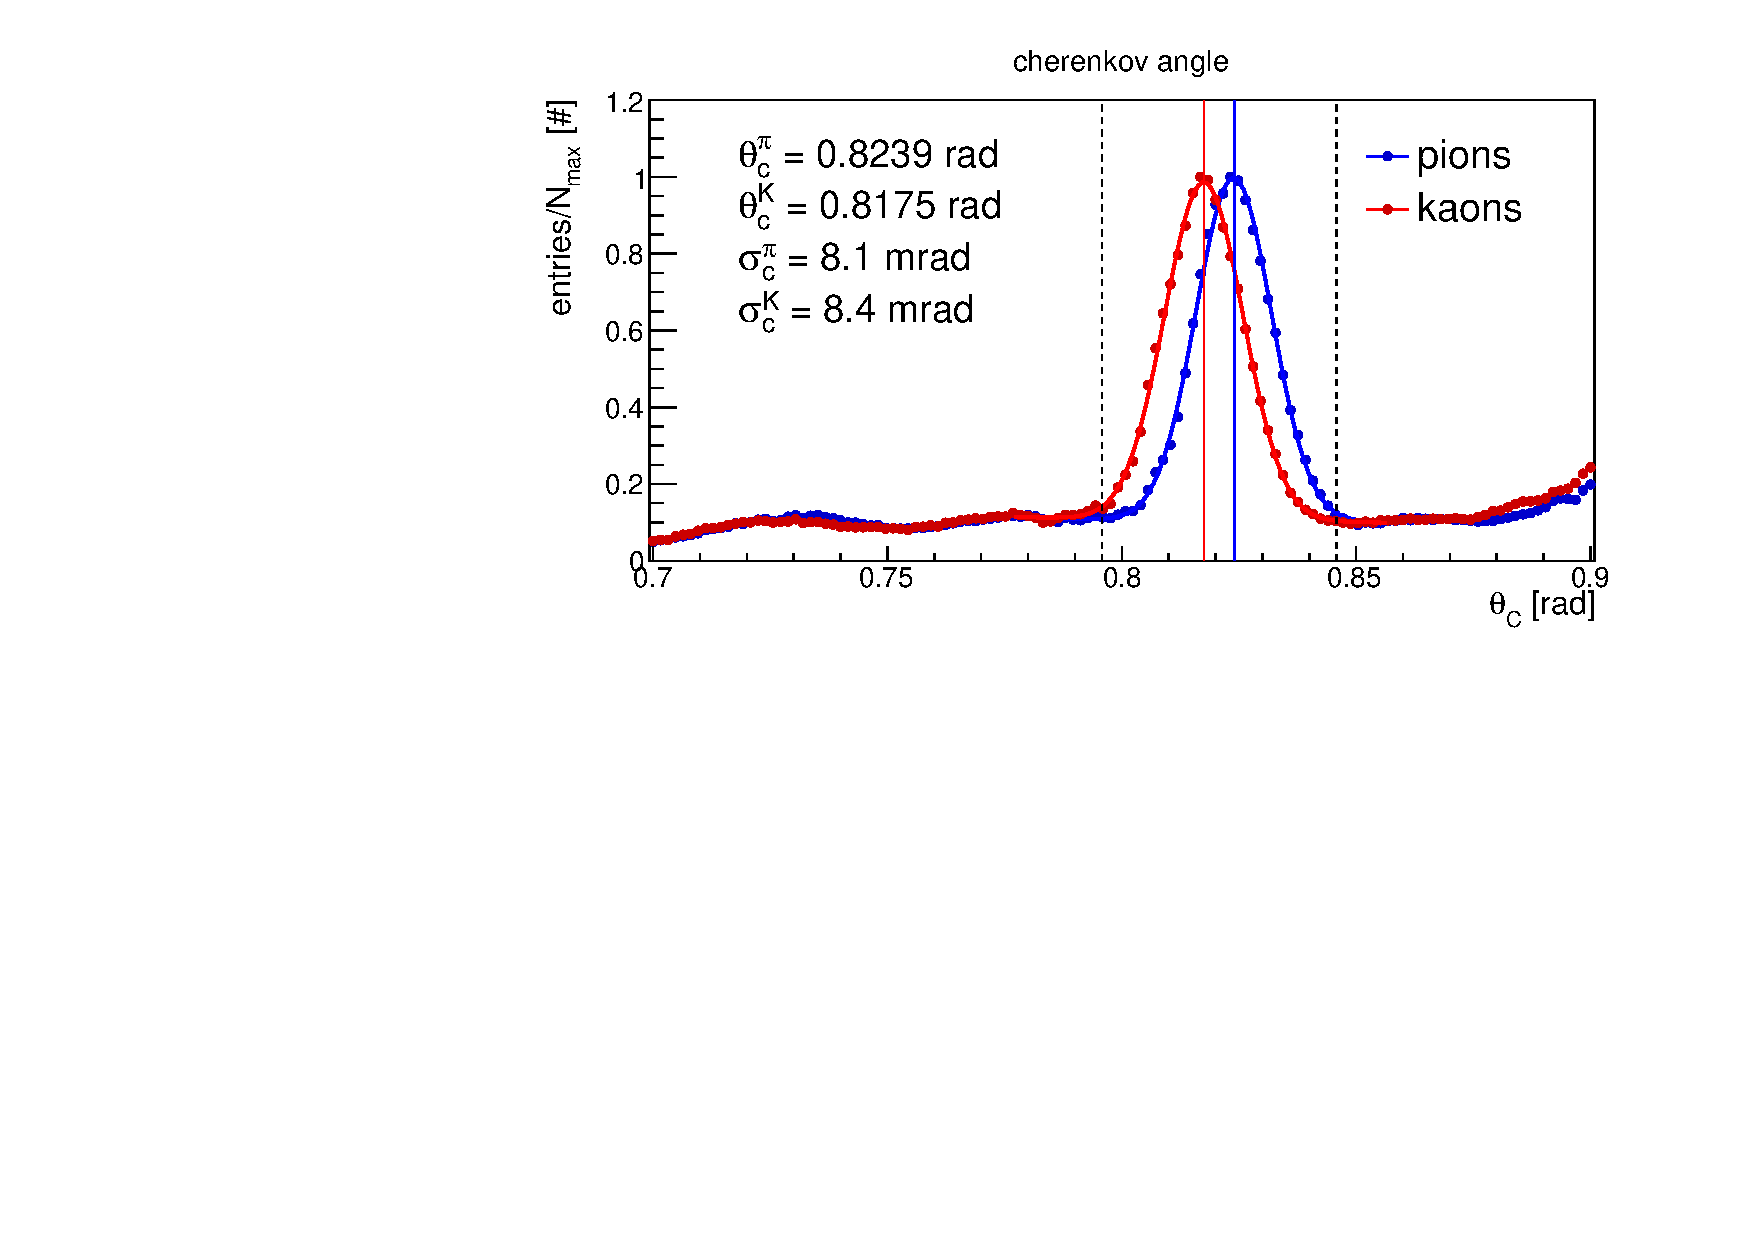
\includegraphics[clip, trim=0cm 0cm 0cm 0.7cm, width=0.8\textwidth]{pics/hAngle.pdf}
\caption{\label{pic:spr}
Cherenkov angles per photon for kaons (red) and pions (blue) with momenta of $4$ {\gev}/c, and direction defined by $\theta = 4$\mydeg and $\phi = 90$\mydeg angles. The solid vertical lines show the expected values for the Cherenkov angles. The dashed lines define the range of values, where the reconstructed photon is considered to be signal (if it also satisfies the cut of time difference). 
%The values of the reconstructed Cherenkov angle and single photon Cherenkov angle resolution are shown.
}
\end{figure}

Going through all hit pixels for the charged particle and collecting the reconstructed Cherenkov angles in a histogram gives a distribution peaking at the expected value of the Cherenkov angle. Figure~\ref{pic:spr} shows the resulting reconstructed Cherenkov angles per photon, including all reconstructed ambiguities, for 1000 pions and kaons with momentum of $4$ {\gev}/c and direction defined by $\theta = 4$\mydeg and $\phi = 90$\mydeg angles. The vertical lines show the expected values for the Cherenkov angle calculated based on the charged particle mass, momentum, and the mean refractive index of fused silica. The width of the peak corresponds to the single photon Cherenkov angle resolution $\sigma_{C}$.

An important advantage of the geometrical reconstruction method is that it delivers a measurement of $\sigma_{C}$. Single photon Cherenkov angle resolution is an useful quantity, as it can be measured experimentally and represents the detector resolution, therefore, can be compared to other DIRC and RICH counters. Furthermore, the algorithm is very fast since the LUTs depend only on the detector geometry and not on the particle properties, and thus can be created prior to event resonstruction.

The Cherenkov angle resolution for a track $\sigma_{\theta_{C}}$ can be approximated as the following:

\begin{equation}
\sigma^{2}_{\theta_{C}} = \sigma^{2}_{tr} + \frac{\sigma^{2}_{C}}{N_{\gamma}},
\end{equation}

\noindent where $\sigma_{tr}$ is the tracking resolution, defined by the tracking system (is estimated to be at the order of $1$ mrad~\cite{tdr}), $\sigma_{C}$ -- single photon Cherenkov angle resolution, $N_{\gamma}$ -- number of detected photons per track (based on the simulation it is expected to be between 30 and 60).

There are two ways to perform the PID with the geometric reconstruction. The first way is to extract the reconstructed Cherenkov angle for a charged particle and compare it to the expected values for different hypotheses. The second method is the direct likelihood test.

Log likelihood method of PID compares the measured DIRC signal to the expected signals for different particle hypotheses. In the geometrical reconstruction, each of $N$ hit pixels has a set of $N_{amb}$ Cherenkov angles. The extended log likelihood probability $\log\mathcal{L}$ for a given charged particle hypothesis $h$ ($h = e, \mu, \pi, K, p$) can be defined as~\cite{staric2}:

\begin{equation}
\log\mathcal{L}_{h} = \sum_{i=1}^{N} \sum_{j=1}^{N^{amb}_{i}} \log \Big( S_{h}^{ij} + B_{h}^{ij} \Big) + \log P_{N}(N_{e}),
\label{eq:ll}
\end{equation}

\noindent where $S^{h}_{ij}$ is the signal distribution for the hypothesis $h$, which is the expected value of the Cherenkov angle for the given particle type and momentum, smeared with the measured single photon Cherenkov angle resolution. The distribution is normalized to have the maximum value at $1$. $B^{h}_{ij}$ is the distribution for background (usually described by a linear function). The function $S^{h}_{ij} + B^{h}_{ij}$ for $h = $ kaon and $h = $ pion obtained from the simulation is shown in Fig.~\ref{pic:spr}. $N_{e} = N_{h} + N_{B}$ is the expected number of detected photons, being a sum of the expected number of signal photons $N_{h}$ for hypothesis $h$ and the expected number of background photons, $N_{B}$. The second term in Eq.~\ref{eq:ll} is the Poisson probability to obtain $N$ photons if the mean is $N_{e}$.
%$P_{N}(N)$ is the probability to get the measured number of Cherenkov photons for this hypothesis based on the distribution of the number of expected photons.
During reconstruction, the log likelihood values for the reconstructed Cherenkov photons are summed up for all hit pixels (including all ambiguities). An example of the result is shown in Fig.~\ref{pic:sepLUT}.

\begin{figure}[!h]
\centering
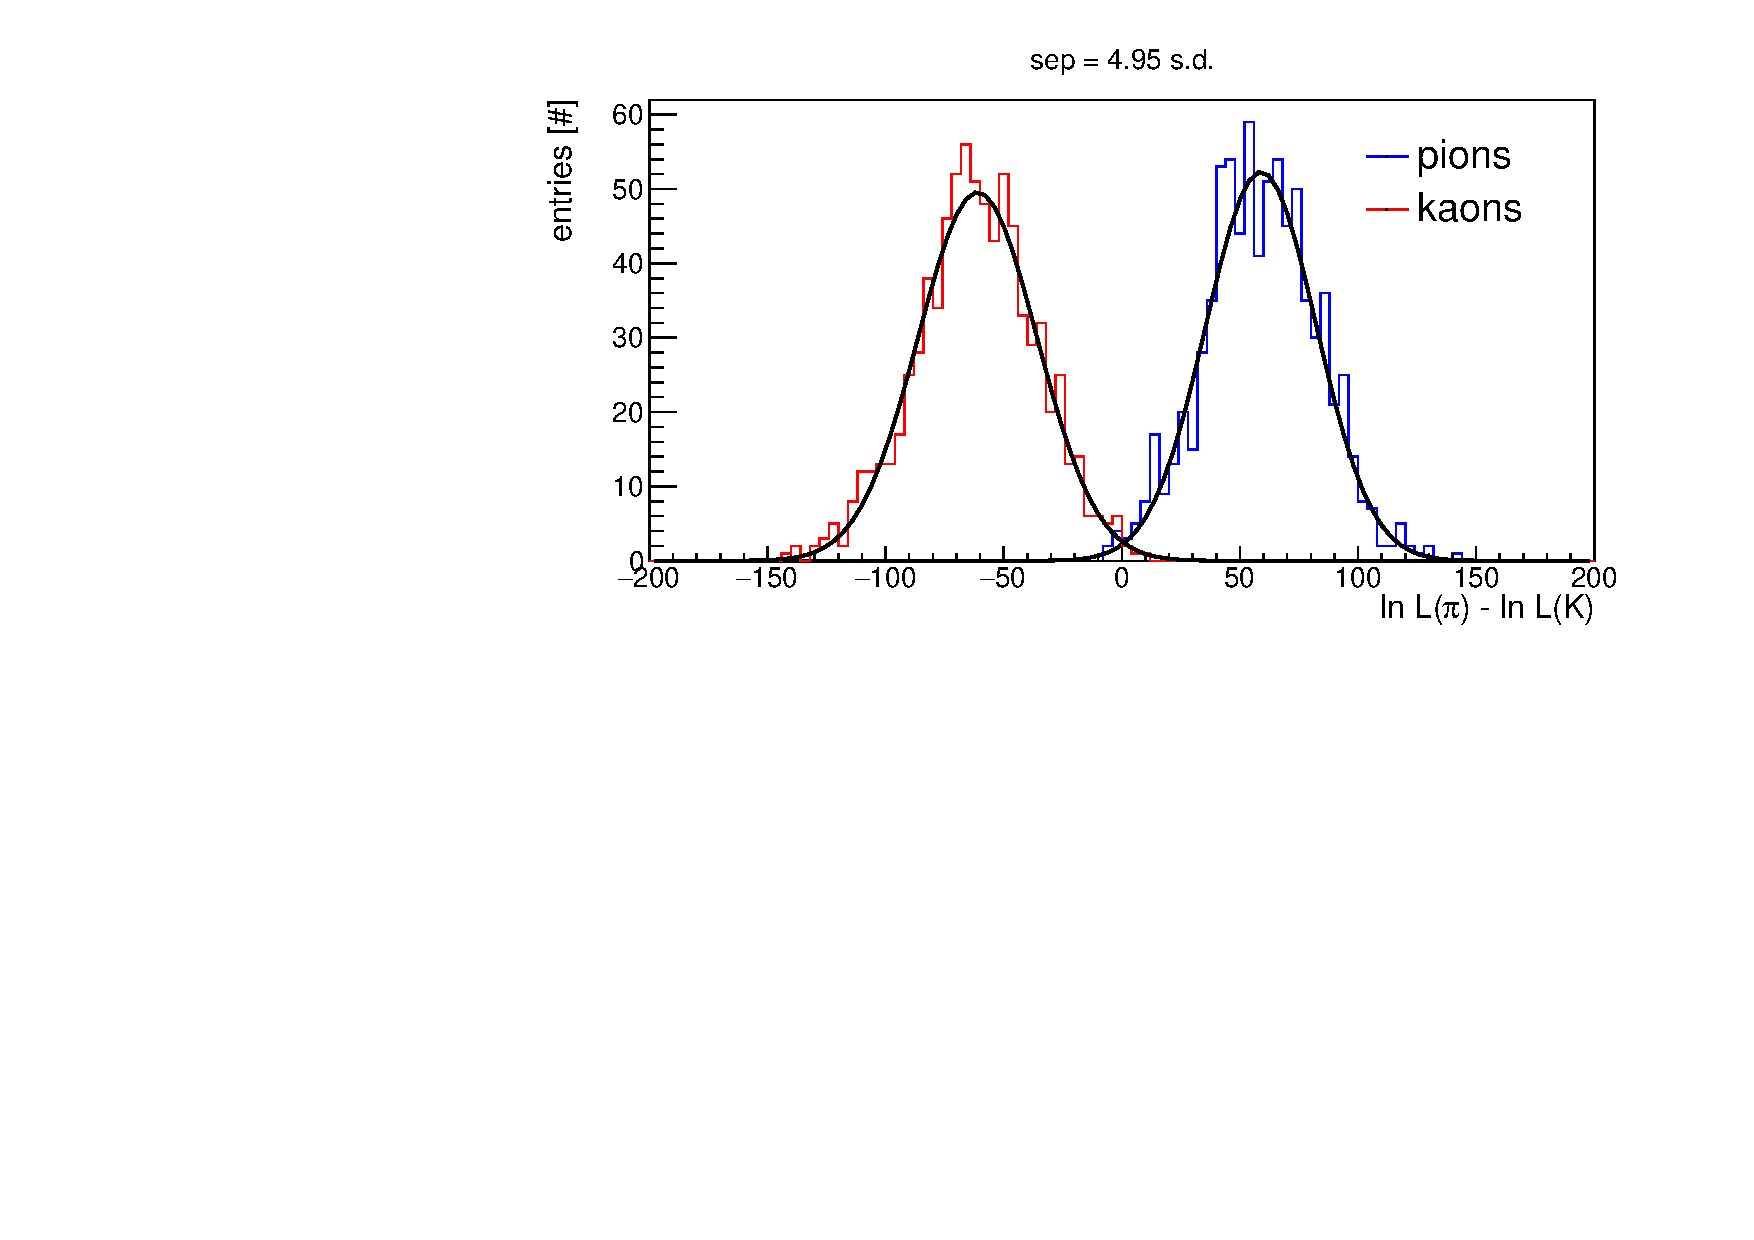
\includegraphics[clip, trim=0cm 0cm 0cm 0.7cm, width=0.8\textwidth]{pics/hLnDiff.pdf}
\caption{\label{pic:sepLUT}
Log likelihoods for kaons (red) and pions (blue) with momenta of $4$ {\gev}/c, and direction defined by $\theta = 4$\mydeg and $\phi = 90$\mydeg is 4.95 s.d.
}
\end{figure}

The separation $S$ between two hypotheses can be calculated based on the difference in log likelihoods:

\begin{equation}
S = \frac{m_{1}-m_{2}}{(\sigma_{1} + \sigma_{2})/2},
\end{equation}

\noindent where $m_{1}$ and $m_{2}$ are the mean values of log likelihoods for two hypotheses, and the denominator shows the average standard deviation assuming the log likelihood distributions are described by Gauss functions with $\sigma_{1}$ and $\sigma_{2}$.


\subsection{Time Imaging Reconstruction}
\label{sec:ti}

The time-based imaging method is based on the approach used by the Belle II time-of-propagation (TOP) counter~\cite{staric2}. The basic concept is that the measured arrival time of Cherenkov photons in each single event is compared to the expected photon arrival time for every pixel and for every particle hypothesis, yielding the PID likelihoods.

The expected photon arrival time, which accounts for the time of flight of particle from interaction region to the fused silica radiator and for the propagation time of the Cherenkov photon produced by that particle in the radiator, can be calculated in different ways:
\begin{itemize}
\item The expected timing spectra can be calculated analytically based on the charged particle momentumn and hit location on the DIRC wall, as desctibed in~\cite{staric2, staric3}.
\item The full detector simulation can be used to produce timing spectra for each photon. Since the DIRC signal depends on the particle momentum, direction, and the position on the DIRC wall, the simulation of timing spectra for all charged particle configurations might be not feasible.
\item In beam tests, when the external PID is available, the timing spectra can be extracted from the data.
\end{itemize}

The second approach was used to evaluate the time-based imaging method for \gluex DIRC.

\begin{figure}[!h]
\centering
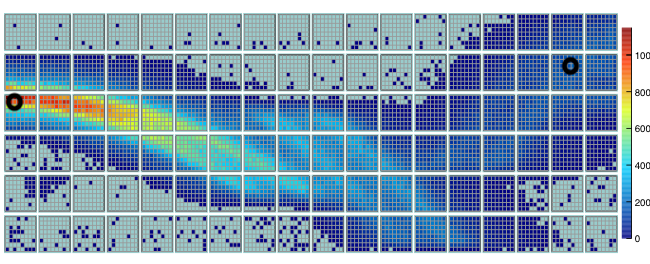
\includegraphics[clip, trim=0cm 0cm 0.5cm 0.1cm, width=0.58\textwidth]{pics/kaonsTI.png} \hspace{0.05\textwidth} \includegraphics[clip, trim=0.75cm 0.35cm 0.35cm 0.52cm,width=0.35\textwidth]{pics/LeftPix.png}
\put(-140.,-8.){\small{photon propagation time [ns]}} \put(-70., 70.){\textcolor{red}{pions}} \put(-70., 50.){\textcolor{blue}{kaons}}  \\
\includegraphics[clip, trim=0cm 0cm 0.5cm 0.1cm, width=0.58\textwidth]{pics/pionsTI.png} \hspace{0.05\textwidth} \includegraphics[clip, trim=0.75cm 0.35cm 0.35cm 0.52cm,width=0.35\textwidth]{pics/rightPix.png} 
\put(-140.,-8.){\small{photon propagation time [ns]}} \put(-70., 70.){\textcolor{red}{pions}} \put(-70., 50.){\textcolor{blue}{kaons}} 
\caption{\label{pic:hitpatKpi}
Hit pattern for kaons (upper left) and pions (bottom left) with momentum of $2$ {\gev}/c and direction defined by $\theta = 1.2$\mydeg and $\phi = 90$\mydeg angles. Black circles mark two pixels, for which timing spectra are shown on the right. The timing spectra for pions (red) and kaons (blue) for the left circled pixel are shown on the upper left plot, and for the right circled pixel -- on the lower right plot.
}
\end{figure}

Figure~\ref{pic:hitpatKpi} illustrates the principle of the time imaging  algorithm. The left column shows cumulative $(x, y)$ hit patterns for pions and kaons with momentum of $2$ {\gev}/c and direction defined by $\theta = 1.2$\mydeg and $\phi = 90$\mydeg angles. The upper hit pattern (kaons) is clearly shifted downward by about half of one PMT with respect to the lower one (pions) illustrating the fact, that these two hypotheses can be well separated. The black circles mark two pixels on the photodetection plane, for which the reference timing spectra are shown on the right. The upper right plot shows time distribution for the left circled pixel, and the lower right plot shows time distribution for the right circled pixel. The red color corresponds to pions, and blue -- to kaons.
 
The DIRC measures the arrival times $t_{i}$ and positions $(x_{i}, y_{i})$ of the $N$ Cherenkov photons detected on the photodetection plane. The extended log likelihood probability $\log\mathcal{L}$ for a given charged particle hypothesis $h$ ($h = e, \mu, \pi, K, p$) can be 
defined as~\cite{staric2}:

\begin{equation}
\log\mathcal{L}_{h} = \sum_{i=1}^{N} \log \Big( S_{h}(x_{i}, y_{i}, t_{i}) + B_{h}(x_{i}, y_{i}, t_{i}) \Big) + \log P_{N}(N_{e}),
\label{eq:ll}
\end{equation}

\noindent where $S_{h} (x_{i}, y_{i}, t_{i})$ is the signal distribution for the hypothesis $h$, i.e. timing spectra for different pixels (see the right column in Fig.~\ref{pic:hitpatKpi}). $B(x_{i}, y_{i}, t_{i})$ is the distribution for background (usually described by a linear function), and $N_{e} = N_{h} + N_{B}$ is the expected number of detected photons, being a sum of the expected number of signal photons $N_{h}$ for hypothesis $h$ and the expected number of background photons, $N_{B}$. The second term in Eq.~\ref{eq:ll} is the Poisson probability to obtain $N$ photons if the mean is $N_{e}$.
Examples of $N_{e}$ are shown in Fig.~\ref{pic:npho}.

\begin{figure}[!b]
\centering
\includegraphics[width=0.8\textwidth]{pics/ll.pdf} \hspace{0.5cm} %\includegraphics[width=0.52\textwidth]{pics/sepTI1000.png}
\caption{\label{pic:sepTI}
Log likelihoods for kaons (red) and pions (blue) with momenta of $4$ {\gev}/c, and direction defined by $\theta = 4$\mydeg and $\phi = 90$\mydeg. 
}
\end{figure}

The normalizations of $S_{h} (x_{i}, y_{i}, t_{i})$ and $B(x_{i}, y_{i}, t_{i})$ for the log likelihoods are:

\begin{equation}
\sum_{j=1}^{n_{ch}} \int_{0}^{t_{m}} S_{h}(x_{j}, y_{j}, t) dt = N_{h}\cdot N_{e},
\label{eq:norm1}
\end{equation}

\begin{equation}
\sum_{j=1}^{n_{ch}} \int_{0}^{t_{m}} B(x_{j}, y_{j}, t) dt = N_{B} \cdot N_{e},
\label{eq:norm2}
\end{equation}

\noindent where the sum runs over all channels $n_{ch}$ of the photon detector array, $(x_{j}, y_{j})$ being detector coordinates, and the integration is performed over the full range $t_{m}$ of the time-of-arrival measurement.

An example of log likelihoods assuming single photon timing resolution of 1 ns is shown in Fig.~\ref{pic:sepTI}.

The separation $S$ between two hypotheses can be calculated based on the difference in log likelihoods.

%The time imaging reconstruction method is sensitive to the single photon timing resolution. Indeed, the timing information is used here directly, unlike for the geometrical algorithm, where only coarse timing information is needed to cut out some solutions of the reconstructed Cherenkov angle. Figure~\ref{pic:sepTI} shows separation between kaons and pions for two values of the single photon timing resolutions. The single photon timing resolution of 1 ns is the current realistic single photons timing resolution.


\newpage

\subsection{KDE-based Reconstruction}
\label{sec:kde}

In order to build a KDE based particle hypothesis PDF, the algorithm must quickly trace many photons from the charged particle path to the detection array.  This provides the $n$ $s_{i}$ in equation~\eqref{eq:kernel_form} in the next section {\em i.e.} it provides the many samples from a PDF required to estimate the PDF with Kernel Density Estimation (KDE).  FastDIRC leverages the symmetry of the bars to trace photons to the detector plane about 10000 times faster than \geant~\cite{Hardin:2016cvu}.

This tracing consists of a generation step, a step that traces through the bars, and a step which traces through the expansion volume.  We use the coordinate system shown in Fig.~\ref{pic:coord}.  The output of FastDIRC is a \deltall which is converted to a resolution as described in Appendix~\ref{app:resolution}.

\begin{figure}[!h]
  \begin{center}
    \includegraphics[width=.35\textwidth]{pics/billi.png}
    \caption{\label{pic:coord} 
      Coordinate system used when discussing the DIRC.  The sign of the $x$ direction is not relevant for reconstruction.}
  \end{center}
\end{figure}

\subsubsection*{Kernel Density Estimation}

One way to produce an estimate of the value of a probability density function at a point is to draw many points from that PDF and spread them with a kernel.  With enough points to resolve features, and a kernel sufficiently wide to provide smoothness, this results in a continuous estimate of the PDF which improves as the number of sampled point increases.  The algorithm presented in~\cite{Hardin:2016cvu} and implemented in FastDIRC generates a PDF in the 2 spatial coordinates (for the image plane) and time.

Let the set of $n$ points $\vec{s}$ be drawn from PDF $P$, then we can approximate $P$  as

\begin{equation}
P(x) \approx \sum_{i}^{n} K(x - s_{i}),
\label{eq:kernel_form}
\end{equation}
where $K$ is a decaying function of distance (often a gaussian), whose width is a decreasing function of the number of support points.  For the \gluex DIRC, the spatial and time resolution of the PMTs provide a natural scale around which to search for a kernel width.  A KDE allows for a continuous estimate of any PDF which can be sampled.

\subsubsection*{Tracing Through the Bars}
A significant hurdle to implementing a KDE estimator via traditional optics is the O(100) internal reflections that each photon undergoes as it propagates though the bar.  As O(600,000) KDE points are required for some hypotheses,\footnote{This number taken from the plateau of 5 GeV K-$\pi$ estimated for \gluex.  Lower energy particles can be well separated with less precise PDFs.} this results in a prohibitive number of multiplications for any large data set.  In order to overcome this, we take advantage of the fact that reflections can be mapped to drawing a straight line through a tiled plane.  Since rectangular prisms provide a simple tiling of the plane, it is only necessary to determine the ratio of the distances the particle travels in the $x-z$ plane to the distance it travels in $y$.  The distance in $y$ is known (this is just the distance to the end of the bar, or the distance through its image on the reflective end), making it easy to reconstruct the number of $x$ and the number of $y$ reflections by using integer division.  The parity of this integer tells us which direction the photon is now moving, while the remainder of the distance gives its position.  Tracing this way requires a constant, small amount of computation per photon to trace to the end of the bar, as opposed to the O(100) internal reflections that might otherwise be required.  See Fig.~\ref{fig:bounces_unfolding}.

\begin{figure}[!h]
\centering
\includegraphics[width=0.45\textwidth]{pics/bouncesLarge.png}
\includegraphics[width=0.54\textwidth]{pics/bouncesUnfolding.png}
\caption{Representation of the path of a photon looking down the $y$ axis of a DIRC bar (left).  Unfolding these bounces onto a grid for fast computation (right).}
\label{fig:bounces_unfolding}
\end{figure}


\subsubsection*{Generation}
While tracing is fast, it is still desirable to improve the speed of the algorithm.  One obvious way to do this is to only trace those photons which will produce a photoelectron {\em i.e.} apply the quantum efficiency before tracing the photon to the PMT plane.  As such, at generation, the Cherenkov wavelength PDF for the given $\beta$ of the particle is combined with the quantum efficiency PDF and the wavelength dependent index of fused silica to produce the PDF of the emission angles of photons.  
%See Fig.~\ref{fig:cerenkov_spectrum} for this distribution.  
This is implemented by a successive MC sampling of the Cherenkov wavelength and the quantum efficiency wavelength distributions.  
The wavelength is then used to compute the index of refraction, which is folded in with the particle speed to get a Cherenkov angle.  
The $\phi$ around the Cherenkov cone is sampled uniformly.

\subsubsection*{Optical Box Tracing}
At the end of the bars, the photons must then be traced to the readout plane.  It is desirable that this be done by dedicated code for speed.  The FastDIRC implementation allows an arbitrary class to perform this tracing.  As implemented for the \gluex optical box, the algorithm takes advantage of the fact that there are a finite number of sequences of reflection off of flat planes that a photon can take.  It then checks the case of each photon and simulates.  The output of this tracing is a point which contains the local $(x,y,t)$ coordinates of the PMT plane.

As this tracing is different for every DIRC geometry, the techniques for the \gluex geometry are discussed here.  In addition to the \gluex geometry, FastDIRC implements the geometry for \babar and the SuperB fDIRC prototype.

The \gluex geometry is a series of planar mirrors with a small number of possible paths for the light to take.  Each mirrored plane  is stored as 4 doubles: $a-d$ in the plane equation: $ax+by+cz=d$ or $\vec{N} \cdot \vec{x} = d$.  These numbers are used to simply and quickly compute plane intersection and reflection using the position and direction vector.  If we let $\vec{v}$ be the normalized direction the photon is moving, and we pick $d$ such that $\vec{N}$ is normalized, then the intersection and reflection of a plane is computed as follows:

\begin{equation}
t = -\frac{d + \vec{N} \cdot \vec{x}}{\vec{N} \cdot \vec{v}}
\end{equation}
\begin{equation}
\vec{x}_{intersect} = \vec{x} + t \cdot \vec{v}
\end{equation}
\begin{equation}
\vec{v}_{reflected} = \vec{v} + 2 \cdot (\vec{N} \cdot \vec{v}) \cdot \vec{N}.
\end{equation}
This computation can be done quickly, and small multiplication savings are had by computing both together.  Coordinates are provisionally intersected individually for testing between possible sequential reflections if the condition is otherwise too computationally intensive.  The computation of $t$ provides the distance which is used for timing information.  These techniques are used in the \gluex optical box simulation to decide which of the three segment mirrors to reflect off of and then perform the reflection.  The other mirrors in the box have their reflections performed by image projection---similar to how the propagation in the bars is done.  If the side mirrors (in the $y-z$ plane) are ignored, then any hit on the PMT plane that is outside the bounds can be reflected back after it touches the plane.  Similarly, by projecting to the image of the PMT plane in the large flat mirror rather than reflecting off of it, minor savings can be had.  See Fig.~\ref{fig:optical_box_optimize}.

\begin{figure}[!h]
\centering
\includegraphics[width=0.7\textwidth]{pics/large_planar_pmt_project.png}
\includegraphics[width=0.7\textwidth]{pics/sidemirror_pmt_reflection.png}
\caption{Projection of the PMT plane in the large mirror (top).  The side mirrors are parallel to a coordinate plane, allowing even fewer multiplications (bottom).}
\label{fig:optical_box_optimize}
\end{figure}

The wedge is a special case; its sides are close enough together that multiple reflections off of them are common.  A strategy similar to the bars can be employed here, though FastDIRC currently implements this by looping in the $x$ direction using the method for the side mirror of the PMT plane, but iterated if the path reflects multiple times.  The wedge also has 2 distinct paths for light to propagate through it.  The light is likely to hit the 30\mydeg side (and totally internally reflect) before it exits the quartz and enters another optical medium (in the case of \gluex, this is water), but sometimes it changes optical media before it reflects off the 30\mydeg plane.  On the PMT plane, this creates a small structure slightly offset from the main pattern that looks somewhat like a mustache.  See Fig.~\ref{fig:wedge_paths}.

\begin{figure}[!h]
\centering
\includegraphics[width=0.48\textwidth]{pics/wedge_paths.pdf}
\caption{Possible light path through the wedge as projected into the $yz$ plane.  The vast majority of photons (dependent on incident particle kinematics) take the normal path with a few entering the water first and making a "Mustache".}
\label{fig:wedge_paths}
\end{figure}

For the implementation of the \gluex optical box, the $z$ intercept with particular planes is used to check where the photon will hit next.  By projecting the path and checking the $z$ bounds of the three planes in the three-segment mirror, the correct target can be obtained.  Similarly, the $z$ position when passing through the large planar mirror is used to reject photons which will not reach the plane (but would have due to the nature of FastDIRC treating the large mirror as nonexistent).

\begin{figure}[!h]
\centering
\includegraphics[width=0.49\textwidth]{pics/dist_cyl_perp_n147.png}
\includegraphics[width=0.49\textwidth]{pics/dist_cyl_perp_n133_edit.pdf}
%\put(-14,3.7){A.U.}
\caption{PDF of photons from a pion parallel to the $z$ axis and with a box that uses quartz as an optical medium and a cylindrical mirror (left).  PDF of the same pion with water as a medium (right).  Note that the ring is slightly wider, and the central mustache is visible.}
\end{figure}
\begin{figure}[!h]
\centering
\includegraphics[width=0.49\textwidth]{pics/dist_cyl_440_n133.png}
\includegraphics[width=0.49\textwidth]{pics/dist_440_cannonical_pion_edit.pdf}
%\put(-14,3.7){A.U.}
\caption{PDF of photons from a pion at $\theta=4$ and $\phi=40$ degrees with a box that uses water as an optical medium on a cylindrical mirror (right).  PDF of photons from the same pion with a three segment mirror in the optical box (right).  Lines are drawn to help the eye connect up the image as it has been broken by reflecting off of non smooth planes.  The mustache is not visible in 2D, as it is under one of the major arcs, but these images are well separated in time.}
\label{fig:cyl_threeseg_recon}
\end{figure}

Shown in Fig.~\ref{fig:cyl_threeseg_recon} are the 4 different paths that the light takes out of the top of the bar along with the breaks where there are discontinuities in mirror angle.  In the cylindrical mirror image, the mustache that comes from the less often taken photon path is also shown.  It does not show up in the three segment mirror image because it is overlapping with one of the broken arcs.  What is not visible in the images is the timing of each of these hits.  The photons hit the plane over O(50 ns), and the PMTs are expected to have timing resolution of 1 ns or better.  While the arcs appear to overlap in 2 dimensions, they are well separated when timing information is added.

\subsubsection*{FastDIRC Implementation}

The FastDIRC code is hosted at~\cite{hardinGithub}.  There are a set of classes implementing tracking through a DIRC and providing an interface for various expansion volumes.  In its default run mode, FastDIRC generates each of a pion and kaon PDF once for a given particle kinematics and then simulates many particles with those kinematics and a normalized photon response.  The current driving program then stores this in a set of ROOT histograms, and a ROOT macro to convert these into an equivalent resolution is provided.  There are a variety of command line options to manipulate the geometry.

%\clearpage

\subsubsection*{Speed and Improvements}
The current algorithm can analyze approximately 3 particles/s on a laptop i7-3720QM 2.6GHz.  This is more than sufficient for design work, but is not sufficient to process large amounts of experimental data as a main algorithm.  Several ways to improve the speed are listed here.

Two methods that reduce the computation time of the lower level functions are faster trigonometric computation and better random sampling.  A profiling program reveals that trigonometry and random sampling are the function calls using the largest amount of CPU time.  The trigonometry can be improved by expanding some of the common calls in Taylor series.  The $\arccos$ call in the generation loop is only evaluated over a small range.  The mersenne twister algorithm used for random sampling is the other major CPU user.  Again, the photon generation uses multiple stages of rejection sampling to determine the wavelength.  Converting the function using inversion sampling would reduce the amount of random calls by more than 65\%.

Aside from low-level improvements, a progressive separation, which only simulates the number of points in the KDE that are required to separate the current image is also possible.  Momentum tested KDE filling would further provide performance gains: it has been observed that for well separated (low momentum) particles, the KDE requires significantly fewer photons before its performance begins to plateau, and in experimental data, many particles are at a momentum lower than the absolute required reach of the PID system.

One last major improvement would be to move to GPU-based computing.  GPUs are optimized for parallel ray tracing, which is exactly the task required to build the KDE.  Not all clusters have these resources available, but this method could take full advantage of those that do.

%\subsubsection{Middle line}

One possible extension of the current algorithm is to numerically calculate the central line through the pattern and use a spreading function around that.  Finding the central line, however, is nontrivial, as points along the curve do not correspond monotonically to the angle that they are emitted at around the Cherenkov cone.

Naively, one might expect that there is a simple correlation between progress along the 4 arcs and the $\phi$ around the Cherenkov cone.  By picking a central Cherenkov angle and removing the uncertainty from the $\theta$, the middle of the path can be traced.  As a function of this $\phi$, in fact, the image is essentially double valued.  See Fig.~\ref{fig:double_dirc_image}.

\begin{figure}[!h]
\centering
\includegraphics[width=0.7\textwidth]{pics/DoubleVals.pdf}
\caption{A single Cherenkov angle with sequential $\phi_{cone}$ values connected.}
\label{fig:double_dirc_image}
\end{figure}

Each half of the image is filled by the 2$\pi$ cycle around the Cherenkov cone.  To account for this, trace the image based only on photons having hit one of the two last $y-z$ sides of the bar {\em i.e.} only trace photons moving in the negative $x$ direction on exiting the bar.  This procedure results in the image in Fig.~\ref{fig:single_tracing}.

\begin{figure}[!h]
\centering
\includegraphics[width=0.7\textwidth]{pics/phi10k.pdf}
\caption{A single Cherenkov angle connecting $\phi_{cone}$ over $[0,2\pi]$ when the photons that bounce off one side plane are not traced.}
\label{fig:single_tracing}
\end{figure}

While the figure has removed the double valued nature, and does not have thickness from the Cherenkov angle spread, it still includes the {\em Kaleidoscope} effect.  The Kaleidoscope effect is the zig-zag pattern that the $\phi$ projection traces along the ring.  It comes from the fact that, when projected onto the grid shown for the bar optimization, the Cherenkov cone makes a parabola with a small part of the arc inside of each rectangle.  That arc corresponds to a finite interval in $\phi$ space and is continuously translated onto the PMT plane.  To get rid of the arcs making this substructure, we decrease the amount of $\phi$ domain they consume by making the bar arbitrarily thin (so that it almost looks like a plane).  While this increases the number of nominal bounces, our propagation time is independent of bounce number, so it has no effect on speed.  Once the photon reaches the top of this wafer, it is adjusted to that its $v_z$ is positive and it is sitting directly in the middle of the top of the bar.  This, combined with the selection for the last wall hit\footnote{As implemented, the last wall hit alternates between adjacent $\phi$, beacuse the last wall is not well defined in an infinitely thin wedge.} produces a smooth line through the middle of the image.  See Fig.~\ref{fig:single_tracing_line}.

\begin{figure}[!h]
\centering
\includegraphics[width=0.7\textwidth]{pics/line_overpoints_2d.pdf}
\caption{The line drawn with 10k $\phi$ points over the half of the pattern it corresponds to.  Again using the $\theta=4\eqdeg$, $\phi=40\eqdeg$ kinematics.}
\label{fig:single_tracing_line}
\end{figure}

The line traces the entire structure save for the mustache.  In this geometry, the mustache can only be produced by a photon close to $z=0$ when it exits the bar.  In the approximation of an infinitely thin bar, the photon is exiting at the middle of the bar.  This is visible in the $y$ versus Cherenkov $\phi$ plot.  This represents a small number of photons, and should minimally impact reconstruction, but it could be corrected by producing another ring in a future study.  The breakdown of the line's path in $x$, $y$, and $t$ appears in Fig.~\ref{fig:single_line_breakout}.

\begin{figure}[!htb]
\centering
\includegraphics[width=0.49\textwidth]{pics/line_overt_v_phi.pdf}
\includegraphics[width=0.49\textwidth]{pics/line_overx_v_phi.pdf}
\includegraphics[width=0.49\textwidth]{pics/line_overy_v_phi.pdf}
\caption{The time of intersection versus Cherenkov $\phi$ (left).  The $x$ location of intersection versus Cherenkov $\phi$ (right).  The $y$ location of intersection versus Cherenkov $\phi$ (bottom).}
\label{fig:single_line_breakout}
\end{figure}

One tested method of using this line to analyze a particle uses 10k initial points to make the line for both a pion and a kaon.  Then each of the experimental hits finds the closest point to it on this line and takes a weighted distance with spreads similar to the kernel of the original KDE.  After some minimal optimization of the parameters of this procedure, the separation returned is approximately 20\% worse than the full simulation with only 2\% as many support points required.  The analysis of possible algorithms leveraging the middle line was left at this point.  The main FastDIRC driver contains code to implement the line.

\clearpage

\subsubsection*{FastDIRC Performance}

FastDIRC as implemented provides for a basic LUT reconstruction implementation using the same information from the PMT plane.  This allows comparison of the two reconstruction methods on an equal footing.  To make the comparison more direct, the output of the LUT was translated to a resolution through the same ROC curve based method as the output of the KDE.  The resolution of FastDIRC over the kinematic region of the DIRC is shown in Fig.~\ref{fig:FastDIRC_performance}.  The performance of the LUT with and without a basic chromatic correction can be seen in Fig.~\ref{fig:lut_performance}.  The comparison of FastDIRC to a LUT is shown in Fig.~\ref{fig:FastDIRC_lut_comparison}.

\begin{figure}[!h]
\centering
\includegraphics[width=0.49\textwidth]{pics/lut_map_chrom.pdf}
\includegraphics[width=0.49\textwidth]{pics/lut_map_nochrom.pdf}
\caption{Resolution from LUT-based reconstruction using a chromatic correction (left).  Same without a chromatic correction (right).}
\label{fig:lut_performance}
\end{figure}

\begin{figure}[!h]
\centering
\includegraphics[width=0.7\textwidth]{pics/kde_map.pdf}
\caption{Resolution from FastDIRC created KDE PDFs.}
\label{fig:FastDIRC_performance}
\end{figure}

\begin{figure}[!h]
\centering
\includegraphics[width=0.7\textwidth]{pics/lut_v_kde_map.pdf}
\caption{Fractional improvement $\left(\frac{\sigma_{LUT}-\sigma_{FastDIRC}}{\sigma_{LUT}}\right)$ in Cherenkov angle resolution when moving from KDE to LUT.}
\label{fig:FastDIRC_lut_comparison}
\end{figure}

The curved zones of worse resolution in these figures correspond to charged particle kinematics which produce significantly overlapped rings.  While there are attempts to improve LUT based reconstruction by more efficiently using timing information, the KDE based reconstruction outperforms this LUT over the entire region, and shows the most improvement where the rings overlap the most.  Sample distributions for all kinematics can be found at~\cite{hardinWebDists}.

The $\approx 30\%$ performance increase is unfortunately still CPU intensive.  Simulating a KDE for each particle is still O(1000) slower than evaluating a LUT despite the O(10000) speedup in tracing particles through the bars.  This is sufficient for design work, but would not permit use as a dedicated reconstruction algorithm as implemented.  The possible improvements detailed above might drive this time down, and it is possible to use a hybrid reconstruction, {\em i.e.} only attempt a KDE based return for sufficiently ambiguous LUT responses.

\subsubsection*{Resolution Definitions}
\label{app:resolution}
The \deltall based KDE method used to do K--$\pi$ separation in this thesis does not return a Cherenkov angle for a given set of hits, but rather a log likelihood difference between particle hypotheses.  If we want to compare this performance using a more physical "resolution," we can obtain a log likelihood difference for many simulated kaons and for many simulated pions.  By plotting the pion veto efficiency versus the kaon identification efficiency for each possible value of a cut on this set of log likelihoods, we obtain a ROC curve.  The integral of this ROC curve gives us a measure of separation performance that can be compared to the performance of a detector which returned an angle spread by a gaussian.  By picking the spread of this gaussian such that the ROC curve of the ideal gaussian detector matches the simulated \deltall ROC curve, we obtain a "matching" resolution for the algorithm.  This matching resolution behaves broadly as expected:  It scales as ${n_{pe}^{-\frac{1}{2}}}$, where $n_{pe}$ is the number of photoelectrons and adds in quadrature with other errors in the system.

\begin{figure}[!h]
\centering
\includegraphics[width=0.49\textwidth]{pics/overlap_5_4_40.pdf}
\includegraphics[width=0.49\textwidth]{pics/roc_curve_overlay_5_4_40.pdf}
\caption{The \deltall difference for pions and kaons plotted against each other at 5~GeV, $\theta=4\eqdeg$, $\phi=40\eqdeg$ (left).  The ROC curve associated with those overlapping histograms (red) and the ROC curve of 2 gaussians with mean separated by the same angle (4.2 mrad) with $\sigma$=1.46 mrad (dotted blue) (right).}
\label{fig:roc_curve}
\end{figure}

%\subsubsection*{Single Photon Resolution}
The ROC curves match well in Fig~\ref{fig:roc_curve}, implying that the performance is close to gaussian.  This extracted resolution has the expected property of varying as ${n_{pe}^{-\frac{1}{2}}}$.  Given this scaling, it is convient to quote a single photon resolution, which is just $\sigma_{res}{n_{pe}^{\frac{1}{2}}}$.


\newpage

\subsection{Simulation Studies and Performance Comparison}
\label{sec:com}

This section discusses the current issues for the existing reconstruction methods and compares the performance between different methods.

\subsubsection{Geometrical Reconstruction}

The geometrical reconstruction was moved from the plugin to a JANA factory within the GlueX software. 

\subsubsection{Time-Based Imaging}

An essential part of the time-based imaging is the expected timing spectra for individual pixels (PDFs for individual pixels). As it was discussed in Section~\ref{sec:ti}, these spectra depend on particle direction and velocity, and can be either calculated analytically or simulated.

%Analytical calculation of the expected timing spectra for each pixel relies on the angular resolution for the charged track. (add later)

%Simulation of the expected timing spectra for each pixel requires reasonable grid over the phase space. The photon yield depends on the angles of the charged particle with respect to the radiator sides, and the particle momentum. But we will use the (x,y) position on the DIRC wall and momentum coordinates for the phase space.

To find out the range of the track directions and positions, which can be reconstructed using the same PDF, two simulation studies were performed. A sample of single kaons and pions with momentum of 4 GeV/$c$ and direction defined by the polar angle of $1.4^{\circ}$ and azimuthal angle of $90^{\circ}$ was generated right in front of the DIRC radiator (x = 0, y = -10.4 cm, z = 585.5 cm) and reconstructed using a set of various PFDs. Figure~\ref{pic:simPDF}a shows the resulting separation between pions and kaons when the position of the charged tracks used for PDF was varied. The angle of the tracks used for PDF was kept the same as for the reconstructed sample. Figure~\ref{pic:simPDF}b shows the case when the direction of the tracks used for PDF was varied. In this case the position of the track origin stayed the same as for the reconstructed sample.

\begin{figure}[!h]
\centering
\includegraphics[clip, trim=0.4cm 0.4cm 0.4cm 0.4cm, width=0.45\textwidth]{pics/xy_scan.pdf} \hspace{0.5cm} \includegraphics[clip, trim=0.4cm 0.4cm 0.4cm 0.4cm, width=0.45\textwidth]{pics/th_phi_scan.pdf}
\caption{\label{pic:simPDF}
Separation power (color axis) for kaons and pions of a single track event sample (momentum of 4 GeV/$c$, $\theta$ = 1.2$^{\circ}$ and $\phi$ = 90$^{\circ}$ generated right in front of the DIRC radiator with x = 10.4 cm and y = 0) using PDFs for various positions (left) or directions (right). The variation of position for the PDFs kept the direction constant and equal to that for the reconstructed sample. The variation of the angles kept the original position of the tracks constant and equal to that of the reconstructed sample.
}
\end{figure}

The simulation studies show that the separation between pions and kaons does not change if the track is reconstructed using a PDF for the same radiator bar, with x position on the DIRC wall within $\pm$ 5 cm from the track position, and within 0.5 degrees in theta and about $\pm$ 10 degrees in phi.



\newpage

\begin{thebibliography}{1}
\bibitem{dirc} F.~Barbosa et al., ``The GlueX DIRC detector'', NIM \textbf{A} 876 (2017) 69.
\bibitem{gluex1} GlueX Collaboration, ``Mapping the Spectrum of Light Quark Mesons and Gluonic Excitations with Linearly Polarized Photons'', Jefferson Lab PAC 30 Proposal, 2006.
\bibitem{gluex2} A.~AlekSejevs et al., GlueX Collaboration, \url{arXiv:1305.1523}.
\bibitem{gluex3} M.~Dugger et al., GlueX Collaboration, \url{arXiv:1408.0215}. 
\bibitem{bdirc1} I.~ Adam et al., NIM \textbf{A} 538 (2005) 235.
\bibitem{fdirc} B.~Dey et al., NIM \textbf{A} 775 (2015) 112.
\bibitem{scalar} H.~Bennet, J.~Elson, and J.~Bennet ``Scattering from optical surfaces'' Vol. 7. Applied Optics and Optical Engineering. Academic Press New York, 1979.
\bibitem{roughness} J.~Cohen-Tanugi et al., ``Optical properties of the DIRC fused silica Cherenkov radiator'', NIM \textbf{A} 515 (2003) 680. 
\bibitem{Epotek} Epoxy Technology, Inc. 14 Fortune Drive Billerica, MA 01821.
\bibitem{EpotekData} BABAR DIRC Note 140 ``Measurement of Epotek-301-2 Optical Glue Refraction Index and Reflectivity from Epotek-301-2/Fused Silica Interface'', J. Va'vra (2001).
\bibitem{deg} P.~Degtyarenko ``Precision analysis of the photomultiplier response to ultra low signals'', NIM \textbf{A} 872 (2017).
\bibitem{borospec}\url{https://www.schott.com/borofloat/english/attribute/optical/index.html}.
\bibitem{slacpub} J.~Va'vra ``Optical properties of RICH detectors'', SLAC-PUB-15942 (2014).
\bibitem{formula}\url{https://www.gelest.com/product/pdv-0331/}.
\bibitem{pcpaper} D.~Motta, S.~Sch{\"o}nert ``Optical properties of bialkali photocathodes'' NIM \textbf{A} 539 (2005) 217. 
\bibitem{water} A.~Morel ``Optical properties of Pure Water and Pure Sea Water'', Academic Press, 1974.
\bibitem{water2} R.~R{\"o}ttgers, ``Measurements of inherent optical properties of pure water'', Technical note, GKSS Forschungszentrum in der Helmholtz Gemeindschaft.
\bibitem{tdr} GlueX Collaboration, ``GlueX DIRC Technical Design Report'', 2015.
\bibitem{staric2} M.~Staric et al., ``Pattern recognition for the time-of-propagation counter'', NIM \textbf{A} 639 (2011) 252.
\bibitem{staric3} M.~Static et al., ``Likelihood analysis of patterns in a time-of-propagation (TOP) counter'', NIM \textbf{A} 595 (2008) 252.
\bibitem{Hardin:2016cvu} J.~Hardin and M.~Williams, ``FastDIRC: a fast Monte Carlo and reconstruction algorithm for DIRC detectors'', JINST 11 (2016).
\bibitem{hardinGithub}\url{https://github.mit.edu/jmhardin/FastDIRC}.
\bibitem{hardinWebDists}\url{www.mit.edu/~jmhardin/worklinks/dirc\_distros.html}.

\end{thebibliography}


\end{document}
